% \documentclass[paper=a4, fontsize=11pt]{scrartcl} % A4 paper and 12pt font size
\documentclass[12pt, a4paper]{book}
\usepackage{lmodern}
\usepackage[spanish, es-tabla]{babel} % Selecciona el español para palabras introducidas automáticamente, p.ej. "septiembre" en la fecha y especifica que se use la palabra Tabla en vez de Cuadro
\decimalpoint
\usepackage{url} % ,href} %para incluir URLs e hipervínculos dentro del texto (aunque hay que instalar href)
\usepackage{graphics,graphicx, float} %para incluir imágenes y colocarlas
\usepackage[gen]{eurosym} %para incluir el símbolo del euro
%\usepackage{cite} %para incluir citas del archivo <nombre>.bib
\usepackage{enumerate}
\usepackage{hyperref}
\usepackage{graphicx}
\usepackage{tabularx}
\usepackage{booktabs}
\usepackage{afterpage}
\usepackage{caption}
\captionsetup[figure]{labelfont={bf,it},textfont={it},font=small,indention=0.5cm}
\captionsetup[table]{labelfont={bf,it},textfont={it},font=small,indention=0.5cm}
\usepackage{natbib}%bibliografia tipo "et al"
\bibliographystyle{plainnat}
\usepackage{multirow} %fusionar celdas en columnas en tablas
\usepackage{colortbl}
\usepackage{hhline}
\usepackage{pdfpages} %insertar pdf en el documento, para la portada
\usepackage{subfigure} % subfiguras
\usepackage{setspace} %espaciado e interlineado
\usepackage{multicol} %varias columnas en una numeracion, capitulo 3


\usepackage{amsmath}%Letras griegas en negrita
%\hypersetup{
%	colorlinks=true,	% false: boxed links; true: colored links
%	linkcolor=black,	% color of internal links
%	urlcolor=cyan		% color of external links
%}
\renewcommand{\familydefault}{\sfdefault}
\usepackage{fancyhdr} % Custom headers and footers
\pagestyle{fancyplain} % Makes all pages in the document conform to the custom headers and footers
\fancyhead[L]{} % Empty left header
\fancyhead[C]{} % Empty center header
\fancyhead[R]{Jaime Jiménez González} % My name
\fancyfoot[L]{} % Empty left footer
\fancyfoot[C]{} % Empty center footer
\fancyfoot[R]{\thepage} % Page numbering for right footer
%\renewcommand{\headrulewidth}{0pt} % Remove header underlines
\renewcommand{\footrulewidth}{0pt} % Remove footer underlines
\setlength{\headheight}{13.6pt} % Customize the height of the header

\usepackage{titlesec, blindtext, color}
\definecolor{gray75}{gray}{0.75}
\newcommand{\hsp}{\hspace{20pt}}
\titleformat{\chapter}[hang]{\Huge\bfseries}{\thechapter\hsp\textcolor{gray75}{|}\hsp}{0pt}{\Huge\bfseries}
\setcounter{secnumdepth}{4}
\usepackage[Lenny]{fncychap}


\begin{document}
% Portada UPM

\setlength{\parskip}{\baselineskip}

\includepdf[pages=-]{Portadas/Portadadefinitiva}

%Agradecimientos
%\thispagestyle{empty}

\chapter*{Agradecimientos}

Se acaba una época, una época dura, con mejores y peores momentos, de los cuales solo lo buenos quedarán en el recuerdo.\\


Aquí quiero agradecerle a todos aquellos que han estado a mi lado su incansable labor de hacerme el camino más fácil, empezando por mi familia, que ha estado ahí en todo momento aportando toda la tranquilidad posible y el apoyo que solo ellos saben dar.\\


También he de agradecer a mis amigos todas las risas y horas de trabajo compartidas, por compartir penas y alegrías que me han ayudado a llegar aquí, tanto a la gente que he conocido nueva, como a la que lleva conmigo desde antes, tanto en la Escuela como fuera de ella.\\


Por último dar las gracias a mi pareja, por haber estado a mi lado en todo momento ayudándome con esta carga hasta cuando parecía inaguantable. Nunca me ha fallado y siempre me ha ayudado a levantarme.\\

Gracias a todos por haberme acompañado y por hacer de esto una realidad.
 
%Desarrollo de Capítulos
\thispagestyle{empty}
\chapter{Introducción}

Como bien es sabido, el desarrollo de una nueva aeronave partiendo de 0 es un trabajo tremendamente complejo que supondría en la industria unos costes desmesurados. Por ello, en este Trabajo de Fin de Grado se plasmará el desarrollo de un diseño preliminar empleando para ello un análisis de vehículos semejantes ya existentes.\\

La aeronave a desarrollar será un UAV de un MTOW de 450kg de peso, por lo que será fundamental desarrollar una pequeña base de datos de aeronaves similares para poder obtener un primer diseño.
En este capítulo se tratarán, además de los objetivos del trabajo, las bases de la mecánica de vuelo de las aeronaves de ala rotatoria de forma sencilla.

\section{Objetivos del Trabajo}

El objetivo principal de este trabajo es generar un diseño preliminar de una aeronave no tripulada de ala rotatoria de un peso máximo al despegue de 450kg. Este diseño, realizado mediante un estudio de aeronaves similares, será después validado por un análisis de sus actuaciones a partir del equilibrado de la misma.
Es justo aquí donde se verá reflejada la originalidad del trabajo, a la hora de elegir las actuaciones a analizar.\\

La validación se llevará a cabo además de forma paralela a una optimización de características de la aeronave, como pueda ser el alcance o la autonomía, en función de otros parámetros de la misma.

Es importante también definir la misión de la aeronave a diseñar, ya que en función de esta optimizaremos unos parámetros u otros y exigiremos unos mínimos a las actuaciones de la misma.


\section{Uso de las Aeronaves no Tripuladas}
Las aeronaves no tripuladas (\emph{\textbf{UAV} \textbf{U}nmanned \textbf{A}erial \textbf{V}ehicle}) están fuertemente ligadas a la aviación militar, siendo esta industria la responsable principal de su desarrollo a lo largo de su historia.
Aunque anteriormente se dieron casos de \emph{UAVs}, como son los globos con los que el ejercito austríaco bombardeó Venecia en 1849, las primeras aeronaves no tripuladas como las conocemos hoy se desarrollaron durante la Primera Guerra Mundial por parte de los Estados Unidos.\\

A día de hoy, y aunque el desarrollo de la tecnología ha sido gracias a la industria militar, más concretamente a la industria militar de Estados Unidos, su uso se ha extendido más allá de esta. Ya no se trata de instrumentos de guerra ni de un artículo de lujo, sino que existen una gran variedad de aeronaves que cumplen distintas funciones fuera de la aviación militar, sino como parte de la aviación comercial civil (como puedan ser las aeronaves radio control cuyo mando puede ser un \emph{smartphone} personal).\\

Algunos de estos usos son los siguientes:

\begin{itemize}
	\item Fotografía y grabación aérea, tanto profesional como recreativa.
	\item Control de daños en zonas afectadas por desastres.
	\item Transporte de mercancías.
	\item Seguimiento y predicción de fenómenos atmosféricos (tornados, tormentas, etc.)
	\item Control y patrulla de fronteras
	\item Inspecciones en zonas de difícil acceso (o imposible).
	\item Entretenimiento
\end{itemize}

Por otro lado siguen creciendo los usos militares;

\begin{itemize}
	\item Combate aéreo
	\item Supervisión y control
	\item Balizas de objetivos
\end{itemize}

Estos son solo algunos de los usos de los \emph{UAVs}, pero la lista crece continuamente.\\

Pese al fuerte desarrollo civil, el principal gasto mundial en aeronaves no tripuladas viene del sector militar, motivado también por el gasto que conllevan los programas militares y los costes de las aeronaves (en 2011, el coste del programa MQ-1 \emph{Predator} era de 2,38 mil milllones de dólares \cite{Predatorunitbudget}, mientras que el coste de una unidad del mismo se sitúa en 4,03 millones de dólares \cite{Predatorprogrambudget}). Se espera un gasto global de 70 mil millones de dólares en aeronaves no tripuladas para 2020 \cite{Goldman}\\

Sin embargo, el sector cuyo crecimiento se espera sea mayor es el civil. Según datos de BI Intelligence, se espera un crecimiento del 19\% en el mercado civil frente a un 5\% en el militar para el período 20015-2020.
Esto se debe principalmente al incremento en la variedad de operaciones que los \emph{UAVs} son capaces de realizar y a su implementación en las empresas. Debido a este crecimiento, se espera también la creación de 100.000 puestos de trabajo solo en Estados Unidos para 2025 \cite{AUVSI}.\\

\section{Mecánica del Vuelo de un Helicóptero}

%A completar posteriormente junto a lo anterior, de vez en cuando escribe algo mamon.

\section[\textbf{HE}licopter and \textbf{RO}tor \textbf{E}quilibrium and \textbf{S}tability toolbox]{HEROES}

%Por aqui explicar que no se harán cálculos directamente, sino que se usará la herramienta. Descripción, sistema de "cajas", incognitas de los problemas, soluciones...

\section{Descripción del Proyecto}

En este caso se ha decidido desarrollar una aeronave ligera cuyo objetivo será abastecer pequeños despliegues militares en zonas de conflicto desde las bases principales. Los convoyes de transporte por tierra han sido atacados durante los últimos años y por ello las tropas han tenido problemas con el abastecimiento de suministros. La idea es que la aeronave sustituya a estos, de manera que el transporte no solo sea más seguro al ser más difícil de interceptar, sino también más rápido y seguro al no contar con tripulación a bordo. 
Los suministros serán principalmente alimentos, aunque sería posible mandar también armamento y suministros sanitarios en caso de necesidad, aunque siempre en pequeñas cantidades, los despliegues a abastecer no serán muy numerosos, y tampoco deberán estar muy alejados de una base principal.

Esto deja claro las características necesarias para la aeronave; 
\begin{itemize}
	\item Una carga de pago máxima lo más alta posible, de manera que resulte eficiente y no sean necesarios múltiples vuelos diarios para un mismo despliegue salvo casos excepcionales.
	\item Una velocidad de crucero buena, de manera que el tiempo que la aeronave esta en vuelo sea el mínimo posible, para evitar así la intercepción. Además también servirá para transportar suministros médicos en caso de emergencia.
	\item Un alcance de unos 400 Km, se manera que pueda abastecer a distancias de alrededor de 200 Km. Es importante que la aeronave pueda realizar el trayecto de ida y vuelta sin repostar, ya que ello obligaría a disponer de combustible en las zonas a abastecer, lo que no es conveniente para la misión. También hay que tener en cuenta que la mitad del trayecto se realizará con la máxima carga de pago la mayoría de las ocasiones, pero la otra mitad la aeronave no tendrá en la mayoría de los casos carga alguna (será posible enviar de vuelta a las bases principales pequeñas cargas en caso de necesidad).
	\item Un techo de vuelo suficiente para dificultar su intercepción, ya que la aeronave no contará con un blindaje militar para priorizar otras características.
\end{itemize}
Como se observa, apenas se han definido numéricamente estas características, ya que en una primera aproximación no se conoce con exactitud la misión, por lo que todos estos parámetros se intentarán maximizar durante el diseño para obtener unas actuaciones lo mejores posible y que la aeronave pueda ser útil en un rango más amplio de situaciones.



\thispagestyle{empty}
\definecolor{Gray}{rgb}{ .949,  .949,  .949}
\newcolumntype{g} {>{\columncolor{Gray}}c}
\chapter{Análisis de Semejantes. Helicóptero Semilla}

Tal y como se ha reflejado en la introducción, el proceso a seguir para optener un diseño preliminar, será el análisis de semejantes.
Este análisis consiste en crear una base de datos de aeronaves ya existentes, cuyas características sean similares a las que podría tener la nuestra, de manera que mediante un análisis estadístico se pueda obtener una primera aproximación de algunas características de nuestra aeronave.\\

\section{Estudio de Aeronaves de Referencia}

Dado que el objetivo es el diseño de un helicóptero no tripulado de 450 Kg de \emph{MTOW}, los vehículos a analizar serán helicópteros de una masa similar, en torno a 400-500 kg, pero al no existir una cantidad suficiente dentro de este margen, se ha decidido ampliar este.
En las tablas \ref{ASomega} y \ref{AS} se encuentran los helicópteros seleccionados para el análisis

%PROBLEMAS CON LAS TABLAS, BUSCAR COMO ARREGLAR EL DESASTRE DE TABLA QUE NO ENTRA, TAL VEZ DIVIDIRLO EN 2 SEA SUFICIENTE
\begin{table}[htbp]
	\centering
	\begin{tabular}{|l|c|c|c|c|c|c|c|}
		\hline
		\rowcolor[rgb]{ .851,  .851,  .851} MODELO & \multicolumn{1}{l|}{MTOW[kg]} & \multicolumn{1}{l|}{d[m]} & \multicolumn{1}{l|}{$\Omega$ [rad/s]} & \multicolumn{1}{l|}{b} & \multicolumn{1}{l|}{$b_a$} & \multicolumn{1}{l|}{$h_{max}$[m]} & \multicolumn{1}{l|}{$V_{max}$[km/h]} \\ \hline
		\rowcolor[rgb]{ .949,  .949,  .949} SA-200 Weasel & \cellcolor[rgb]{ 1,  1,  1}70 & \cellcolor[rgb]{ 1,  1,  1}2,07 & \cellcolor[rgb]{ 1,  1,  1}167,55 & \cellcolor[rgb]{ 1,  1,  1}2 & \cellcolor[rgb]{ 1,  1,  1}6 & \cellcolor[rgb]{ 1,  1,  1}3100 & \cellcolor[rgb]{ 1,  1,  1}167 \\
		\hline
		\rowcolor[rgb]{ .949,  .949,  .949} Yamaha R-50 & \cellcolor[rgb]{ 1,  1,  1}90 & \cellcolor[rgb]{ 1,  1,  1}3,07 & \cellcolor[rgb]{ 1,  1,  1}88,6 & \cellcolor[rgb]{ 1,  1,  1}2 & \cellcolor[rgb]{ 1,  1,  1}2 & \cellcolor[rgb]{ 1,  1,  1}300 & \cellcolor[rgb]{ 1,  1,  1}VACÍO \\
		\hline
		\rowcolor[rgb]{ .949,  .949,  .949} R-350 & \cellcolor[rgb]{ 1,  1,  1}150 & \cellcolor[rgb]{ 1,  1,  1}3,5 & \cellcolor[rgb]{ 1,  1,  1}82,86 & \cellcolor[rgb]{ 1,  1,  1}3 & \cellcolor[rgb]{ 1,  1,  1}2 & \cellcolor[rgb]{ 1,  1,  1}2500 & \cellcolor[rgb]{ 1,  1,  1}120 \\
		\hline
		\rowcolor[rgb]{ .949,  .949,  .949} SD 150 Hero & \cellcolor[rgb]{ 1,  1,  1}150 & \cellcolor[rgb]{ 1,  1,  1}3,5 & \cellcolor[rgb]{ 1,  1,  1}105,14 & \cellcolor[rgb]{ 1,  1,  1}3 & \cellcolor[rgb]{ 1,  1,  1}2 & \cellcolor[rgb]{ 1,  1,  1}4000 & \cellcolor[rgb]{ 1,  1,  1}90 \\
		\hline
		\rowcolor[rgb]{ .949,  .949,  .949} APID 55 & \cellcolor[rgb]{ 1,  1,  1}160 & \cellcolor[rgb]{ 1,  1,  1}3,3 & \cellcolor[rgb]{ 1,  1,  1}54,54 & \cellcolor[rgb]{ 1,  1,  1}2 & \cellcolor[rgb]{ 1,  1,  1}2 & \cellcolor[rgb]{ 1,  1,  1}3000 & \cellcolor[rgb]{ 1,  1,  1}90 \\
		\hline
		\rowcolor[rgb]{ .949,  .949,  .949} APID 60 & \cellcolor[rgb]{ 1,  1,  1}180 & \cellcolor[rgb]{ 1,  1,  1}3,3 & \cellcolor[rgb]{ 1,  1,  1}90,97 & \cellcolor[rgb]{ 1,  1,  1}2 & \cellcolor[rgb]{ 1,  1,  1}2 & \cellcolor[rgb]{ 1,  1,  1}3000 & \cellcolor[rgb]{ 1,  1,  1}110 \\
		\hline
		\rowcolor[rgb]{ .949,  .949,  .949} Camcopter S100 & \cellcolor[rgb]{ 1,  1,  1}200 & \cellcolor[rgb]{ 1,  1,  1}3,4 & \cellcolor[rgb]{ 1,  1,  1}130,73 & \cellcolor[rgb]{ 1,  1,  1}2 & \cellcolor[rgb]{ 1,  1,  1}2 & \cellcolor[rgb]{ 1,  1,  1}5500 & \cellcolor[rgb]{ 1,  1,  1}222 \\
		\hline
		\rowcolor[rgb]{ .949,  .949,  .949} Pelícano & \cellcolor[rgb]{ 1,  1,  1}200 & \cellcolor[rgb]{ 1,  1,  1}3,3 & \cellcolor[rgb]{ 1,  1,  1}81,22 & \cellcolor[rgb]{ 1,  1,  1}2 & \cellcolor[rgb]{ 1,  1,  1}2 & \cellcolor[rgb]{ 1,  1,  1}3600 & \cellcolor[rgb]{ 1,  1,  1}180 \\
		\hline
		\rowcolor[rgb]{ .949,  .949,  .949} DP 5X Wasp & \cellcolor[rgb]{ 1,  1,  1}227 & \cellcolor[rgb]{ 1,  1,  1}3,2 & \cellcolor[rgb]{ 1,  1,  1}127,33 & \cellcolor[rgb]{ 1,  1,  1}4 & \cellcolor[rgb]{ 1,  1,  1}4 & \cellcolor[rgb]{ 1,  1,  1}4100 & \cellcolor[rgb]{ 1,  1,  1}160 \\
		\hline
	\end{tabular}%
	\caption{Valores de diferentes parámetros de las aeronaves empleadas para el análisis de semejantes cuyos valores de velocidad de giro del rotor principal han sido publicados.}
	\label{ASomega}
\end{table}%

\begin{table}[htbp]
	\centering
	\begin{tabular}{|l|c|c|c|c|c|c|}
		\hline
		\rowcolor[rgb]{ .851,  .851,  .851} MODELO & \multicolumn{1}{l|}{MTOW[kg]} & \multicolumn{1}{l|}{d[m]} & \multicolumn{1}{l|}{b} & \multicolumn{1}{l|}{$b_a$} & \multicolumn{1}{l|}{$h_{max}$[m]} & \multicolumn{1}{l|}{$V_{max}$[km/h]} \\
		\hline
		\rowcolor[rgb]{ .949,  .949,  .949} Scout B1-100 & \cellcolor[rgb]{ 1,  1,  1}77 & \cellcolor[rgb]{ 1,  1,  1}3,2 & \cellcolor[rgb]{ 1,  1,  1}2 & \cellcolor[rgb]{ 1,  1,  1}2 & \cellcolor[rgb]{ 1,  1,  1}VACÍO & \cellcolor[rgb]{ 1,  1,  1}VACÍO \\
		\hline
		\rowcolor[rgb]{ .949,  .949,  .949} Neo S300 & \cellcolor[rgb]{ 1,  1,  1}85 & \cellcolor[rgb]{ 1,  1,  1}3 & \cellcolor[rgb]{ 1,  1,  1}3 & \cellcolor[rgb]{ 1,  1,  1}2 & \cellcolor[rgb]{ 1,  1,  1}VACÍO & \cellcolor[rgb]{ 1,  1,  1}VACÍO \\
		\hline
		\rowcolor[rgb]{ .949,  .949,  .949} Skeldar V-200 & \cellcolor[rgb]{ 1,  1,  1}235 & \cellcolor[rgb]{ 1,  1,  1}4,6 & \cellcolor[rgb]{ 1,  1,  1}2 & \cellcolor[rgb]{ 1,  1,  1}2 & \cellcolor[rgb]{ 1,  1,  1}3500 & \cellcolor[rgb]{ 1,  1,  1}140 \\
		\hline
		\rowcolor[rgb]{ .949,  .949,  .949} Tanan EADS & \cellcolor[rgb]{ 1,  1,  1}300 & \cellcolor[rgb]{ 1,  1,  1}5 & \cellcolor[rgb]{ 1,  1,  1}2 & \cellcolor[rgb]{ 1,  1,  1}2 & \cellcolor[rgb]{ 1,  1,  1}4000 & \cellcolor[rgb]{ 1,  1,  1}150 \\
		\hline
		\rowcolor[rgb]{ .949,  .949,  .949} SVU-200 & \cellcolor[rgb]{ 1,  1,  1}360 & \cellcolor[rgb]{ 1,  1,  1}4,92 & \cellcolor[rgb]{ 1,  1,  1}4 & \cellcolor[rgb]{ 1,  1,  1}2 & \cellcolor[rgb]{ 1,  1,  1}4200 & \cellcolor[rgb]{ 1,  1,  1}209 \\
		\hline
		\rowcolor[rgb]{ .949,  .949,  .949} Cicare 7B & \cellcolor[rgb]{ 1,  1,  1}430 & \cellcolor[rgb]{ 1,  1,  1}6,28 & \cellcolor[rgb]{ 1,  1,  1}2 & \cellcolor[rgb]{ 1,  1,  1}2 & \cellcolor[rgb]{ 1,  1,  1}3000 & \cellcolor[rgb]{ 1,  1,  1}194 \\
		\hline
		\rowcolor[rgb]{ .949,  .949,  .949} Robinson R-22 & \cellcolor[rgb]{ 1,  1,  1}622 & \cellcolor[rgb]{ 1,  1,  1}7,67 & \cellcolor[rgb]{ 1,  1,  1}2 & \cellcolor[rgb]{ 1,  1,  1}2 & \cellcolor[rgb]{ 1,  1,  1}4267 & \cellcolor[rgb]{ 1,  1,  1}188 \\
		\hline
		\rowcolor[rgb]{ .949,  .949,  .949} VSR700 & \cellcolor[rgb]{ 1,  1,  1}680 & \cellcolor[rgb]{ 1,  1,  1}7,2 & \cellcolor[rgb]{ 1,  1,  1}3 & \cellcolor[rgb]{ 1,  1,  1}7 & \cellcolor[rgb]{ 1,  1,  1}3600 & \cellcolor[rgb]{ 1,  1,  1}187 \\
		\hline
		\rowcolor[rgb]{ .949,  .949,  .949} Brantly B-2 & \cellcolor[rgb]{ 1,  1,  1}757 & \cellcolor[rgb]{ 1,  1,  1}7,24 & \cellcolor[rgb]{ 1,  1,  1}3 & \cellcolor[rgb]{ 1,  1,  1}2 & \cellcolor[rgb]{ 1,  1,  1}3290 & \cellcolor[rgb]{ 1,  1,  1}161 \\
		\hline
		\rowcolor[rgb]{ .949,  .949,  .949} Schweizer 300 & \cellcolor[rgb]{ 1,  1,  1}930 & \cellcolor[rgb]{ 1,  1,  1}8,2 & \cellcolor[rgb]{ 1,  1,  1}3 & \cellcolor[rgb]{ 1,  1,  1}2 & \cellcolor[rgb]{ 1,  1,  1}4300 & \cellcolor[rgb]{ 1,  1,  1}176 \\
		\hline
	\end{tabular}%
	\caption{Valores de diferentes parámetros de las aeronaves empleadas para el análisis de semejantes cuyos valores de velocidad de giro del rotor principal no han sido publicados.}
	\label{AS}
\end{table}%



Una vez se ha obtenido la selección de aeronaves semejantes, se procede a realizar un análisis estadístico de las distintas características de los mismos para obtener unos primeros valores de diseño. Al ser la característica más definitoria de la aeronave el peso máximo al despegue, se observará la evolución de los distintos parámetros con el MTOW.
En este capítulo se pueden observar las gráficas que se obtienen del análisis anterior para cada parámetro, incluyendo una línea de tendencia que nos permita obtener una primera aproximación en el diseño. Cabe indicar que se han omitido, en las gráficas correspondientes, aquellos vehículos cuyas características no eran conocidas, sin eliminarlos del resto de ellas. Las líneas de tendencia se han generado usando una aproximación lineal, lo cual puede llevar a una mala aproximación dependiendo de los datos.


\begin{figure}
	\centering
	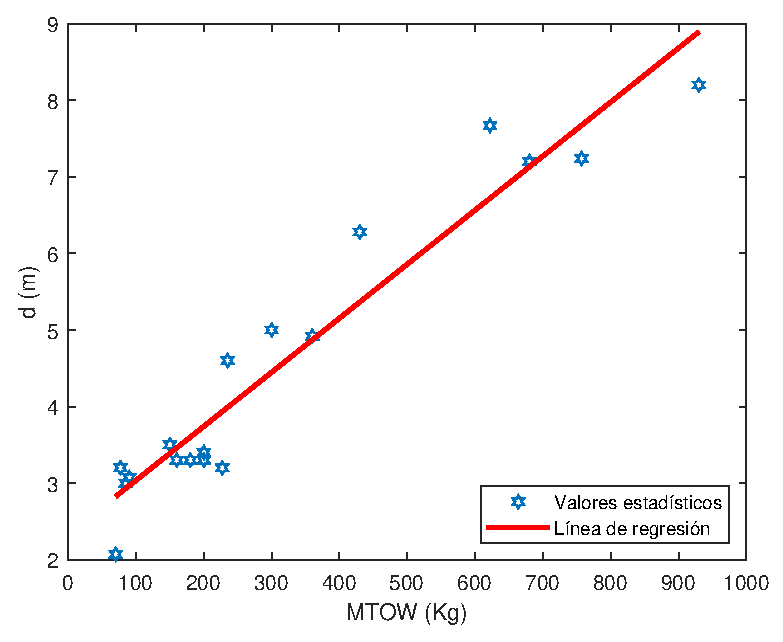
\includegraphics[width=80mm]{graficos/anald}
	\caption{Relación entre los diámetros de las palas de los helicópteros y sus MTOW junto a su línea de tendencia.}
	\label{diamAS}
\end{figure}
\begin{figure}
	\centering
	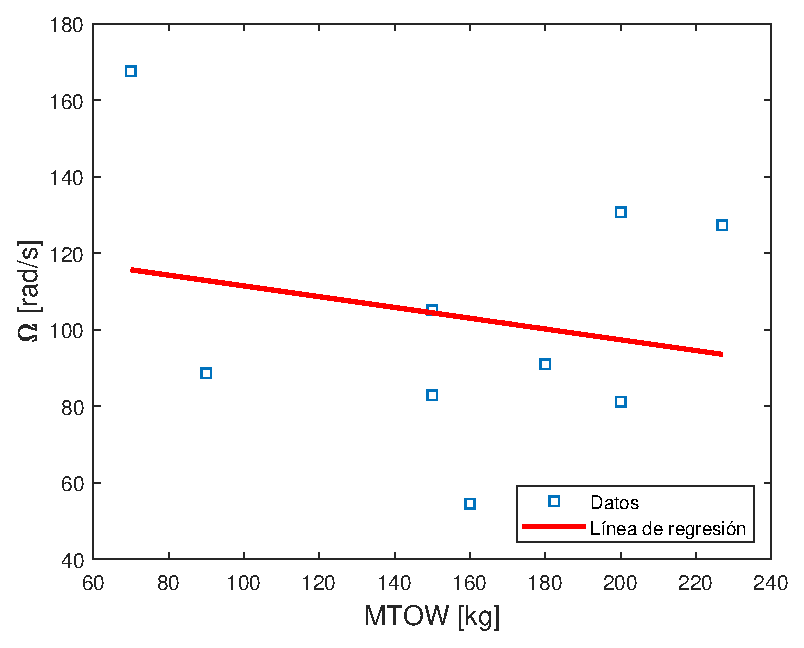
\includegraphics[width=80mm]{graficos/analomega}
	\caption{Relación entre las velocidades de giro del rotor de los helicópteros y sus MTOW junto a su línea de tendencia.}
	\label{omegaAS}
\end{figure}
\begin{figure}
	\centering
	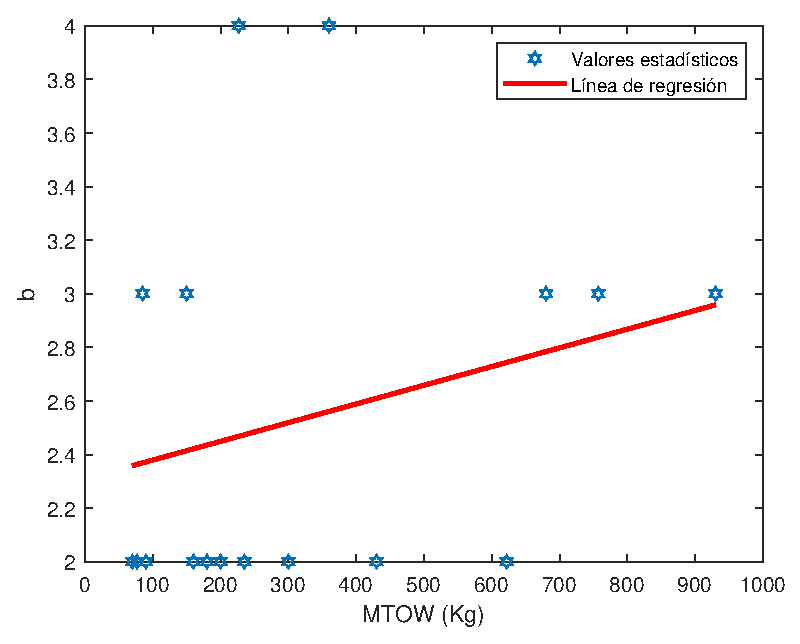
\includegraphics[width=80mm]{graficos/analb}
	\caption{Relación entre el número de palas del rotor principal de los helicópteros y sus MTOW junto a su línea de tendencia.}
	\label{bAS}
\end{figure}
\begin{figure}
	\centering
	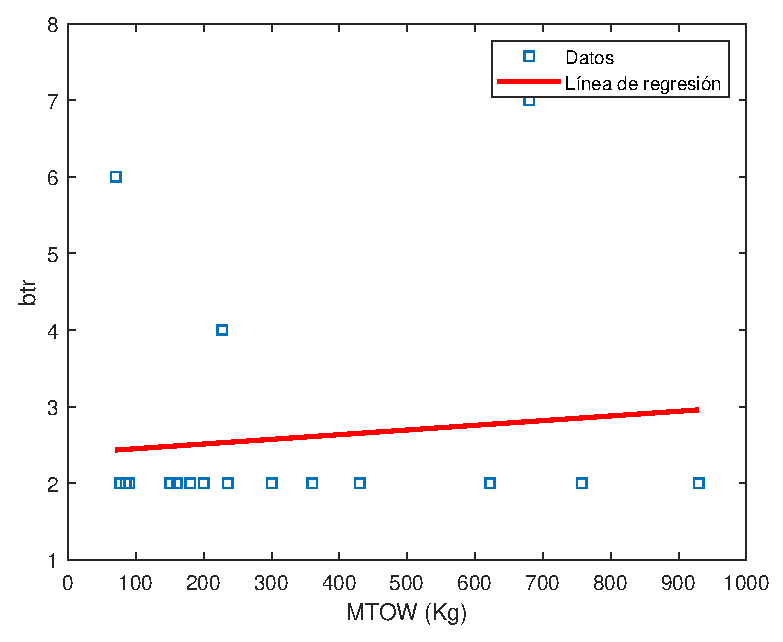
\includegraphics[width=80mm]{graficos/analbtr}
	\caption{Relación entre el número de palas del rotor antipar de los helicópteros y sus MTOW junto a su línea de tendencia.}
	\label{baAS}
\end{figure}
\begin{figure}
	\centering
	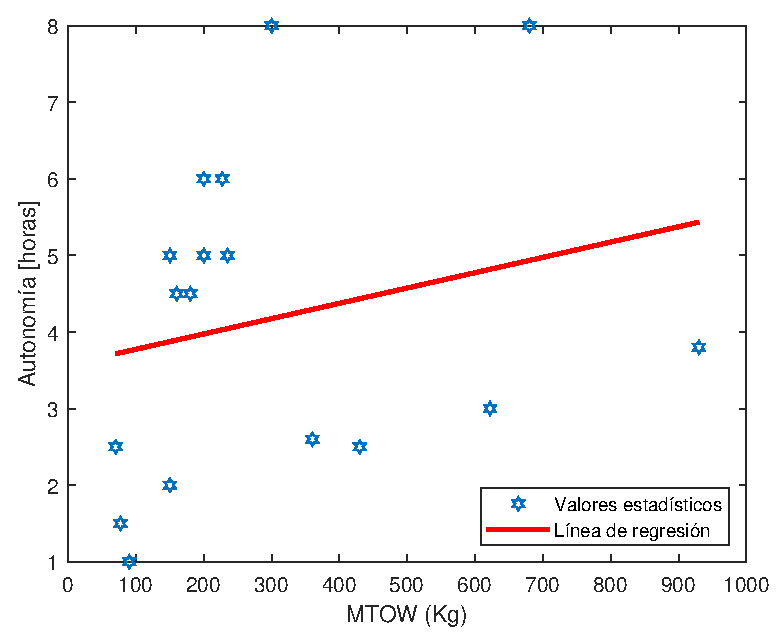
\includegraphics[width=80mm]{graficos/analaut}
	\caption{Relación entre las autonomías de los helicópteros y sus MTOW junto a su línea de tendencia.}
	\label{autAS}
\end{figure}
\begin{figure}
	\centering
	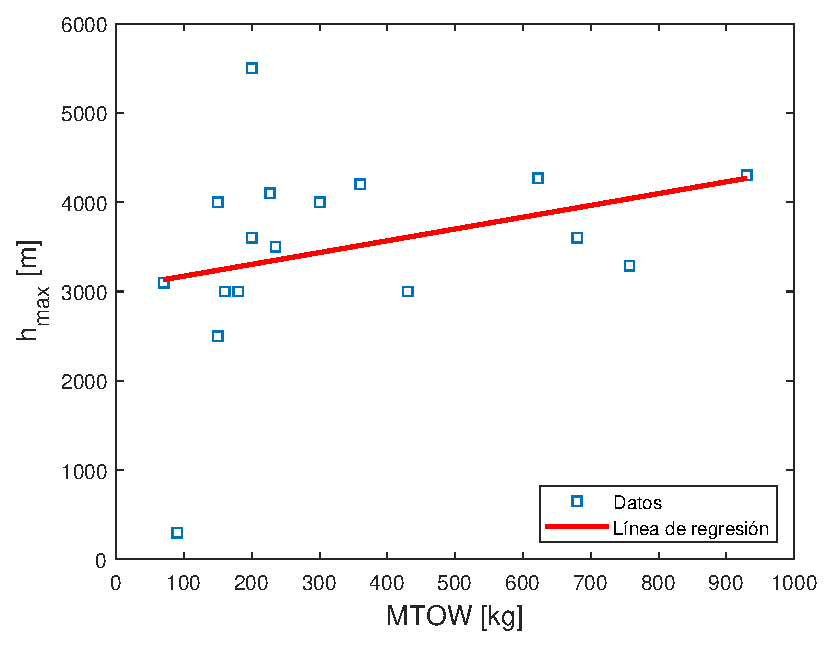
\includegraphics[width=80mm]{graficos/analtecho}
	\caption{Relación entre los techos de vuelo de los helicópteros y sus MTOW junto a su línea de tendencia.}
	\label{techoAS}
\end{figure}
\begin{figure}
	\centering
	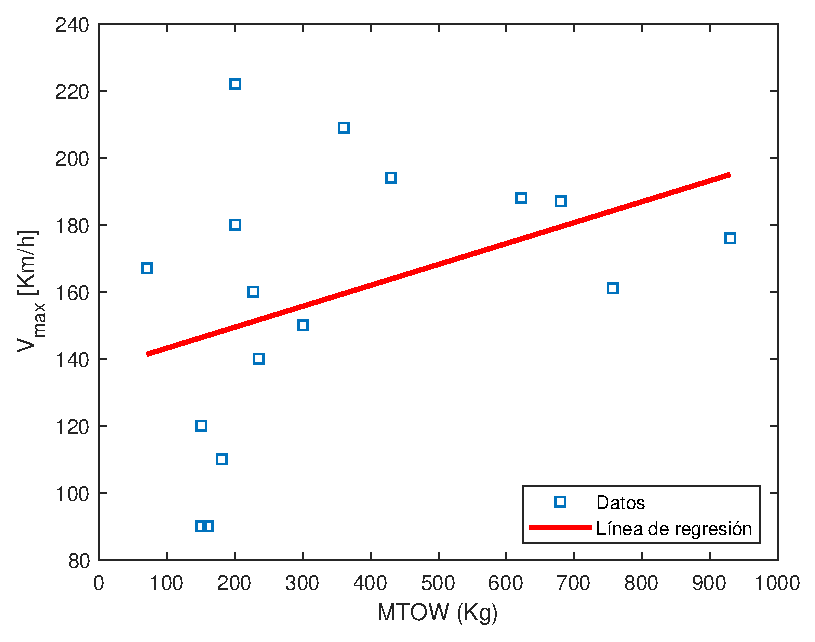
\includegraphics[width=80mm]{graficos/analv}
	\caption{Relación entre las velocidades máximas de avance de los helicópteros y sus MTOW junto a su línea de tendencia.}
	\label{vAS}
\end{figure}

Como se puede observar, muchos helicópteros comparten características aunque sus pesos sean muy distintos, y algunas líneas de tendencia se alejan considerablemente de los valores promedio para la zona que corresponde a 450 kg. Esto se debe principalmente a la falta de datos de referencia, los pocos desarrollos que se han dado de aeronaves de ala rotatoria en el entorno de pesos dado dificultan en gran medida la verificación de nuestro modelo al no existir una norma de diseño en la que basarnos. Los desarrollos han sido dispersos, así que los parámetros iniciales de diseño no se basarán únicamente en los valores de tendencia obtenidos.
 
\begin{itemize}
	\item $d$: 5,5 m
	\item $\Omega$: 120 rad/s
	\item $b$: 2
	\item $b_{a}$ antipar: 2
	\item $t_{e}$: 3 horas
	\item $h_{max}$: 3200 m
	\item $V_{max}$: 190 m/s
\end{itemize}

Queda patente que en algunos casos, se han aproximado los valores omitiendo las líneas de tendencia, usando en su lugar los valores de los helicópteros cuyos MTOW son más próximos al de la aeronave a diseñar.

\section{Descripción Helicóptero Base}

Para poder realizar una simulación en \emph{HEROES} se empleará un helicóptero base que nos ayudará a obtener un modelo preliminar de forma mucho más rápida. Los requisitos de esta aeronave serán que resulte semejante al diseño que se busca, de manera que pueda reescalarse según las necesidades. Para este proyecto se ha escogido el Bölkow Bo 105, un helicóptero utilitario monorrotor, cuyas características se exponen a continuación.

\subsection{Rotor Principal del Bo 105}

Los parámetros necesarios para definir el rotor principal de un helicóptero incluyen datos geométricos, aerodinámicos y de inercia. Los correspondientes al Bo 105 se encuentran recogidos en la tabla \ref{RPBo}.
Para simplificar los cálculos, la pala se modeliza como sólido rígido, unida al rotor por un muelle de constante $k_\beta$.
Además el tensor de inercia de la pala se ha modelizado de la siguiente manera.

\begin{equation}
[I_B]=\left[	
\begin{array}{ccc}
I_\beta & 0 & 0\\
0 & I_\theta & 0\\
0 & 0 & I_\zeta
\end{array}
\right]
\end{equation}

\begin{table}[htbp]
	\centering
	\begin{tabular}{|>{\columncolor{Gray}}c|c|}
		\hline
		\cellcolor{Gray}Radio de las palas ($R$) & \cellcolor[rgb]{ 1,  1,  1}4.91 $m$ \\ \hline
		\cellcolor{Gray}Excentricidad ($e$)& \cellcolor[rgb]{ 1,  1,  1}0 $m$ \\ \hline
		\cellcolor{Gray}Número de palas ($b$) & \cellcolor[rgb]{ 1,  1,  1}4 \\ \hline
		\cellcolor{Gray}Torsión lineal de los perfiles ($\theta_1$) & \cellcolor[rgb]{ 1,  1,  1}-0.14 \\ \hline
		\cellcolor{Gray}Pendiente de la curva de sustentación ($\alpha$) & \cellcolor[rgb]{ 1,  1,  1}6.113 $rad^{-1}$ \\ \hline
		\cellcolor{Gray} & \cellcolor[rgb]{ 1,  1,  1}0.0074 \\ \hhline{|~|-|}
		\cellcolor{Gray} & \cellcolor[rgb]{ 1,  1,  1}0.00961 $rad^{-1}$ \\ \hhline{|~|-|}
		\multirow{-3}{*}{\cellcolor{Gray}Parámetros de la polar ($\delta_0$, $\delta_1$, $\delta_2$)} & \cellcolor[rgb]{ 1,  1,  1}0.29395 $rad^{-2}$ \\ \hline
		\cellcolor{Gray}Velocidad de giro del rotor ($\Omega$) & \cellcolor[rgb]{ 1,  1,  1}44.4 $rad/s$ \\ \hline
		\cellcolor{Gray}Cuerda del perfil ($c$) & \cellcolor[rgb]{ 1,  1,  1}6.113 \\ \hline
		\cellcolor{Gray}Momento de inercia de la pala en batimiento ($I_\beta$) & \cellcolor[rgb]{ 1,  1,  1}231.7 $kgm^2$ \\ \hline
		\cellcolor{Gray}Momento de inercia de la pala en paso ($I_\theta$) & \cellcolor[rgb]{ 1,  1,  1}7 $kgm^2$ \\ \hline
		\cellcolor{Gray}Momento de inercia de la pala en arrastre ($I_\zeta$) & \cellcolor[rgb]{ 1,  1,  1}238.7 $kgm^2$ \\ \hline
		\cellcolor{Gray}Posición del centro de gravedad de la pala ($X_{GB}$) & \cellcolor[rgb]{ 1,  1,  1}2.445 $m$ \\ \hline
		\cellcolor{Gray}Masa de la pala ($m_b$) & \cellcolor[rgb]{ 1,  1,  1}40.2 $kg$ \\ \hline
		\cellcolor{Gray}Rigidez en batimiento ($I_\beta$) & \cellcolor[rgb]{ 1,  1,  1}113330 $Nm/rad$ \\ \hline
	\end{tabular}%
	\caption{Valores de diferentes parámetros del rotor principal de la aeronave Bölkow Bo 105.}
	\label{RPBo}
\end{table}%

\subsection{Rotor Antipar del Bo 105}

Los parámetros necesarios para definir el rotor antipar de un helicóptero son los mismos que definen el rotor principal, y pueden encontrarse en la tabla \ref{RaBo}.
Las mismas consideraciones aplicadas al rotor principal a la hora de modelizarlo se aplican al rotor antipar. Además se considera que la masa de la pala se encuentra uniformemente distribuida a lo largo de la envergadura de la misma y que la unión resulta infinitamente rígida en batimiento.
\begin{table}[htbp]
	\centering
	\begin{tabular}{|>{\columncolor{Gray}}c|c|}
		\hline
		\cellcolor{Gray}Radio de las palas ($R$) & \cellcolor[rgb]{ 1,  1,  1}0.95 $m$ \\ \hline
		\cellcolor{Gray}Excentricidad ($e$)& \cellcolor[rgb]{ 1,  1,  1}0 $m$ \\ \hline
		\cellcolor{Gray}Número de palas ($b$) & \cellcolor[rgb]{ 1,  1,  1}2 \\ \hline
		\cellcolor{Gray}Torsión lineal de los perfiles ($\theta_1$) & \cellcolor[rgb]{ 1,  1,  1}0 \\ \hline
		\cellcolor{Gray}Pendiente de la curva de sustentación ($\alpha$) & \cellcolor[rgb]{ 1,  1,  1}5.7 $rad^{-1}$ \\ \hline
		\cellcolor{Gray} & \cellcolor[rgb]{ 1,  1,  1}0.008 \\ \hhline{|~|-|}
		\cellcolor{Gray} & \cellcolor[rgb]{ 1,  1,  1}0.0096 $rad^{-1}$ \\ \hhline{|~|-|}
		\multirow{-3}{*}{\cellcolor{Gray}Parámetros de la polar ($\delta_0$, $\delta_1$, $\delta_2$)} & \cellcolor[rgb]{ 1,  1,  1}0.294 $rad^{-2}$ \\ \hline
		\cellcolor{Gray}Velocidad de giro del rotor ($\Omega$) & \cellcolor[rgb]{ 1,  1,  1}232.4779 $rad/s$ \\ \hline
		\cellcolor{Gray}Cuerda del perfil ($c$) & \cellcolor[rgb]{ 1,  1,  1}0.18 $m$ \\ \hline
		\cellcolor{Gray}Momento de inercia de la pala en batimiento ($I_\beta$) & \cellcolor[rgb]{ 1,  1,  1}1.805 $kgm^2$ \\ \hline
		\cellcolor{Gray}Momento de inercia de la pala en paso ($I_\theta$) & \cellcolor[rgb]{ 1,  1,  1}0.0648 $kgm^2$ \\ \hline
		\cellcolor{Gray}Momento de inercia de la pala en arrastre ($I_\zeta$) & \cellcolor[rgb]{ 1,  1,  1}1.8698 $kgm^2$ \\ \hline
		\cellcolor{Gray}Posición del centro de gravedad de la pala ($X_{GB}$) & \cellcolor[rgb]{ 1,  1,  1}0.475 $m$ \\ \hline
		\cellcolor{Gray}Masa de la pala ($m_b$) & \cellcolor[rgb]{ 1,  1,  1}6 $kg$ \\ \hline
		\cellcolor{Gray}Rigidez en batimiento ($I_\beta$) & \cellcolor[rgb]{ 1,  1,  1}$10^{100}$ $Nm/rad$ \\ \hline
	\end{tabular}%
	\caption{Valores de diferentes parámetros del rotor antipar de la aeronave Bölkow Bo 105.}
	\label{RaBo}
\end{table}%

\subsection{Fuselaje del Bo 105}

Los parámetros mas relevantes del fuselaje serán aquellos necesarios para la adimensionalización de las fuerzas y momentos sobre el mismo, es decir, las superficies de referencia y la longitud del fuselaje $l_f$.Estos datos se recogen en la tabla \ref{FBo}.

\begin{table}[htbp]
	\centering
	\begin{tabular}{|>{\columncolor{Gray}}c|c|}
		\hline
		\cellcolor{Gray}Longitud del fuselaje ($l_f$) & \cellcolor[rgb]{ 1,  1,  1}8.56 $m$ \\ \hline
		\cellcolor{Gray}Superficie en planta del fuselaje ($S_p$)& \cellcolor[rgb]{ 1,  1,  1}7.5 $m^2$ \\ \hline
		\cellcolor{Gray}Superficie lateral del fuselaje ($S_l$) & \cellcolor[rgb]{ 1,  1,  1}8.3 \\ \hline
		\cellcolor{Gray}Factor de interferencia del rotor principal sobre el fuselaje ($k_f$) & \cellcolor[rgb]{ 1,  1,  1}1 \\ \hline
		\end{tabular}%
	\caption{Valores de los parámetros del fuselaje de la aeronave Bölkow Bo 105.}
	\label{FBo}
\end{table}%

\subsection{Estabilizadores del Bo 105}

Los parámetros que definen a los estabilizadores vertical y horizontal se encuentran recogidos en la tabla \ref{EBo}. Se puede observar que son datos similares a los que tendrían las alas de un avión, obviando los controles e hipersustentadores, ya que aerodinámicamente funcionan de la misma manera, solo que las fuerzas que generan ayudan a aumentar la estabilidad de la aeronave o reducir la potencia del rotor antipar, entre otras funciones.
Se han hecho las consideraciones de que no tienen estrechamiento, son rectos y están formados por un único perfil, motivo por el que el número de parámetros es tan reducido.
En el caso del estabilizador horizontal, este se divide en dos partes, por lo que la superficie corresponde únicamente a la mitad del mismo

\begin{table}[htbp]
	\centering
	\begin{tabular}{|>{\columncolor{Gray}}c|c|}
		\hline
		\cellcolor{Gray}Cuerda del estabilizador vertical ($c_{ev}$) & \cellcolor[rgb]{ 1,  1,  1}0.3 $m$ \\ \hline
		\cellcolor{Gray}Superficie del estabilizador vertical ($S_{ev}$)& \cellcolor[rgb]{ 1,  1,  1}0.805 $m^2$ \\ \hline
		\cellcolor{Gray}Ángulo de calado del estabilizador vertical ($\theta_{ev}$) & \cellcolor[rgb]{ 1,  1,  1}0.0812 $rad$ \\ \hline
		\cellcolor{Gray}Cuerda del estabilizador horizontal ($c_{ev}$) & \cellcolor[rgb]{ 1,  1,  1}0.4 $m$ \\ \hline
		\cellcolor{Gray}Superficie del estabilizador horizontal/2 ($S_{ev}$)& \cellcolor[rgb]{ 1,  1,  1}0.4015 $m^2$ \\ \hline
		\cellcolor{Gray}Ángulo de calado del estabilizador horizontal ($\theta_{ev}$) & \cellcolor[rgb]{ 1,  1,  1}0.0698 $rad$ \\ \hline
	\end{tabular}%
	\caption{Valores de diferentes parámetros de los estabilizadores vertical y horizontal de la aeronave Bölkow Bo 105. La superficie del estabilizador horizontal corresponde a la mitad ya que el mismo esta dividido en 2 partes.}
	\label{EBo}
\end{table}%

\subsection{Inercia del Bo 105}

Para finalizar con la descripción del helicóptero, la tabla \ref{InBo} refleja los datos acerca de la inercia del mismo.

\begin{table}[htbp]
	\centering
	\begin{tabular}{|>{\columncolor{Gray}}c|c|}
		\hline
		\cellcolor{Gray}Peso del helicóptero ($W$) & \cellcolor[rgb]{ 1,  1,  1}21560 $N$ \\ \hline
		\cellcolor{Gray}Momento de inercia del eje $x$ ($I_{x}$) & \cellcolor[rgb]{ 1,  1,  1}1433 $kg\cdot m^2$ \\ \hline
		\cellcolor{Gray}Momento de inercia del eje $y$ ($I_{y}$) & \cellcolor[rgb]{ 1,  1,  1}4973 $kg\cdot m^2$ \\ \hline
		\cellcolor{Gray}Momento de inercia del eje $z$ ($I_{z}$) & \cellcolor[rgb]{ 1,  1,  1}4099 $kg\cdot m^2$ \\ \hline
		\cellcolor{Gray}Producto de inercia $xy$ ($I_{xy}$)& \cellcolor[rgb]{ 1,  1,  1}0 $kg\cdot m^2$ \\ \hline
		\cellcolor{Gray}Producto de inercia $xz$ ($I_{xz}$)& \cellcolor[rgb]{ 1,  1,  1}660 $kg\cdot m^2$ \\ \hline
		\cellcolor{Gray}Producto de inercia $yz$ ($I_{yz}$)& \cellcolor[rgb]{ 1,  1,  1}0 $kg\cdot m^2$ \\ \hline
	\end{tabular}%
	\caption{Valores de inercia de la aeronave Bölkow Bo 105.}
	\label{InBo}
\end{table}%

\section{Limitaciones a la Velocidad de Giro del Rotor}

Como se puede observar, al existir muy pocos datos respecto a las velocidades de giro del rotor principal de los helicópteros elegidos, la obtención de una $\Omega$ inicial ha de obtenerse de algún otro modo. Uno de ellos es la limitación del $M_{crit}$ en la punta de las palas del rotor principal, que es la que se desarrollará a continuación.

La limitación en la velocidad de giro del rotor viene dada por la aparición de efectos supersónicos en las puntas de las palas del mismo. Estos efectos, como puedan ser ondas de choque, empeoran el comportamiento de las palas, pueden hacerlas entrar en pérdida e incluso provocar daños estructurales debido a cargas elevadas.
Por esto es común establecer un límite conocido como $M_{crit}$ basado en la velocidad $\Omega$*R, es decir, la velocidad de avance de las puntas de las palas. Este límite suele ser del orden de 0,4 para vuelo estacionario y 0,8 para vuelo en avance. 


\begin{figure}
	\centering
	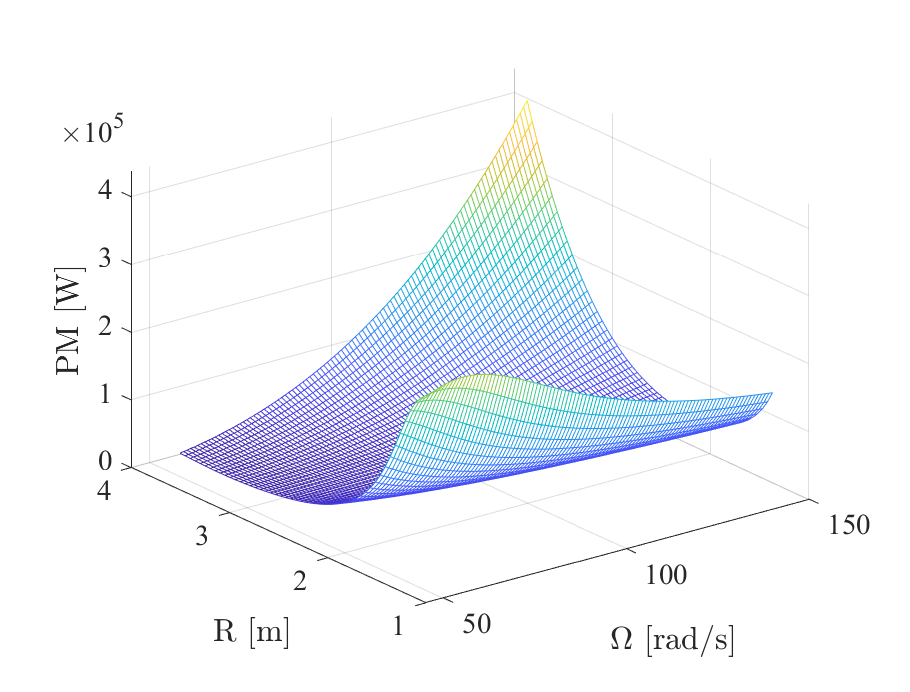
\includegraphics[width=80mm]{graficos/3d3d}
	\caption{Consumo de Potencia de la aeronave en función de la velocidad de giro del rotor y el radio del mismo.}
	\label{ORP}
\end{figure}
\begin{figure}
	\centering
	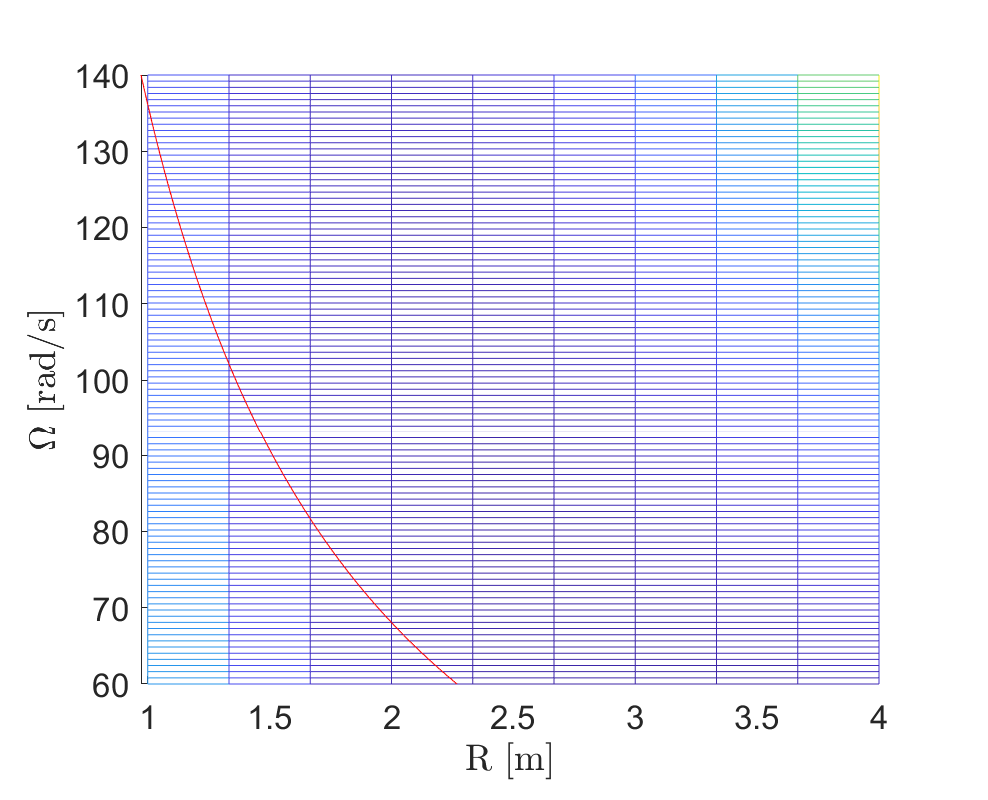
\includegraphics[width=80mm]{graficos/3d2d2}
	\caption{Consumo de Potencia de la aeronave en función de la velocidad de giro del rotor y el radio del mismo junto a la limitación de $\Omega$ a causa del $M_{crit}$ (0,4).}
	\label{ORPM}
\end{figure}

La gráfica \ref{ORP} representa la superficie que da un valor de potencia de la aeronave para cada $\Omega$ y R del rotor. Con esto es posible observar los valores mínimos de potencia, lo que nos permite elegir unos valores de $\Omega$ y R que optimicen la potencia necesaria.
Sin embargo, al añadir la limitación del $M_{crit}$ las opciones de configuración disponibles se ven reducidas a aquellas que la cumplan. La gráfica \ref{ORPM} representa la superficie de la gráfica \ref{ORP} sobre el plano $\Omega$R y encima la anterior limitación.
Se observa claramente que los valores de potencia necesaria se reducen con la potencia y con el aumento de radio, por lo que en primera instancia el menor valor dado, quedando automáticamente definido el radio del rotor.
\begin{itemize}
	\item Velocidad de giro del rotor principal $\Omega$ = 60 $rad/s$
	\item Radio del rotor principal $R$ = 2.26 $m$
\end{itemize}

\section{Helicóptero Semilla}

Con este helicoptero semilla se pueden realizar unas primeras simulaciones de vuelo para comprobar si es válido y, en caso contrario, modificar el diseño para alcanzar unos resultados mejores.

\thispagestyle{empty}

\chapter{Desarrollo de un Helicóptero Semilla a Partir de un Helicóptero Base}

\spacing{1.5}

Comenzar el desarrollo del vehículo desde el principio supondría un esfuerzo y trabajo innecesarios, por lo que lo ideal es la obtención de un helicóptero semilla, un modelo que sirva de primera aproximación sobre el que trabajar y hacer modificaciones. Este helicóptero semilla se obtendrá mediante una adimensionalización de las características de un vehículo real y posterior dimensionalización empleando los parámetros que deba poseer el nuevo vehículo.

Todo este proceso se describirá a lo largo de este capítulo de manera que una vez terminado se tengan los datos necesarios para poder comenzar a realizar simulaciones de vuelo.

\section{Descripción Helicóptero Base}

El primer paso es elegir un modelo que sirva de base para nuestros cálculos y permita obtener un primer diseño lo mas cercano posible al resultado que se desee. El requisito más importante que debe cumplir esta aeronave será que resulte semejante al diseño que se busca, de manera que pueda reescalarse según las necesidades. Para este proyecto se ha escogido el Bölkow Bo 105, un helicóptero utilitario monorrotor, cuyas características se exponen a continuación. Cabe indicar que todos los parámetros definidos conformarán una estructura en MATLAB que se empleará en los cálculos.

\subsection{Rotor Principal del Bo 105}

Los parámetros necesarios para definir el rotor principal de un helicóptero incluyen datos geométricos, aerodinámicos y de inercia. Los correspondientes al Bo 105 se encuentran recogidos en la tabla \ref{RPBo}.
Para simplificar los cálculos, la pala se modeliza como sólido rígido, unida al rotor por un muelle de constante $k_\beta$.
Además el tensor de inercia de la pala se ha modelizado de la siguiente manera:

\begin{equation}
[I_B]=\left[	
\begin{array}{ccc}
I_\beta & 0 & 0\\
0 & I_\theta & 0\\
0 & 0 & I_\zeta
\end{array}
\right]
\end{equation}

\begin{table}[]
	\centering
	\begin{tabular}{|>{\columncolor{Gray}}c|c|}
		\hline
		Radio de las palas ($R$) & 4.91 m \\ \hline
		Excentricidad ($e$) & 0 m \\ \hline
		Número de palas ($b$) & 4 \\ \hline
		Torsión lineal de los perfiles ($\theta_1$) & -0.14 \\ \hline
		Pendiente de la curva de sustentación ($\alpha$) & 6.113 rad$^{-1}$ \\ \hline
		\cellcolor{Gray} & 0.0074 \\ \cline{2-2} 
		\cellcolor{Gray} & 0.00961 rad$^{-1}$ \\ \cline{2-2} 
		\multirow{-3}{*}{\cellcolor{Gray}Parámetros de la polar ($\delta_0$, $\delta_1$, $\delta_2$)} & 0.29395 rad$^{-2}$ \\ \hline
		Velocidad de giro del rotor ($\Omega$) & 44.4 rad/s \\ \hline
		Cuerda del perfil ($c$) & 6.113 m \\ \hline
		Momento de inercia de la pala en batimiento ($I_\beta$) & 231.7 kgm$^2$ \\ \hline
		Momento de inercia de la pala en paso ($I_\theta$) & 7 kgm$^2$ \\ \hline
		Momento de inercia de la pala en arrastre ($I_\zeta$) & 238.7 kgm$^2$ \\ \hline
		Posición del centro de gravedad de la pala ($x_{GB}$) & 2.445 m \\ \hline
		Masa de la pala ($m_b$) & 40.2 kg \\ \hline
		Rigidez en batimiento ($k_\beta$) & 113330 Nm/rad \\ \hline
	\end{tabular}
	\caption{Valores de diferentes parámetros del rotor principal de la aeronave Bölkow Bo 105.}
	\label{RPBo}
\end{table}

\subsection{Rotor Antipar del Bo 105}

Los parámetros necesarios para definir el rotor antipar de un helicóptero son los mismos que definen el rotor principal, y pueden encontrarse en la tabla \ref{RaBo}.
Las mismas consideraciones aplicadas al rotor principal a la hora de modelizarlo se aplican al rotor antipar. Además se considera que la masa de la pala se encuentra uniformemente distribuida a lo largo de la envergadura de la misma y que la unión resulta infinitamente rígida en batimiento.
\begin{table}[htbp]
	\centering
	\begin{tabular}{|>{\columncolor{Gray}}c|c|}
		\hline
		Radio de las palas ($R$) & 0.95 m \\ \hline
		Excentricidad ($e$) & 0 m \\ \hline
		Número de palas ($b$) & 2 \\ \hline
		Torsión lineal de los perfiles ($\theta_1$) & \cellcolor[rgb]{ 1,  1,  1}0 \\ \hline
		Pendiente de la curva de sustentación ($\alpha$) & 5.7 rad$^{-1}$ \\ \hline
		\cellcolor{Gray} & 0.008 \\ \cline{2-2}
		\cellcolor{Gray} & 0.0096 rad$^{-1}$ \\ \cline{2-2}
		\multirow{-3}{*}{\cellcolor{Gray}Parámetros de la polar ($\delta_0$, $\delta_1$, $\delta_2$)} & 0.294 rad$^{-2}$ \\ \hline
		Velocidad de giro del rotor ($\Omega$) & \cellcolor[rgb]{ 1,  1,  1}232.4779 rad/s \\ \hline
		Cuerda del perfil ($c$) & \cellcolor[rgb]{ 1,  1,  1}0.18 m \\ \hline
		Momento de inercia de la pala en batimiento ($I_\beta$) & 1.805 kgm$^2$ \\ \hline
		Momento de inercia de la pala en paso ($I_\theta$) & 0.0648 kgm$^2$ \\ \hline
		Momento de inercia de la pala en arrastre ($I_\zeta$) & 1.8698 kgm$^2$ \\ \hline
		Posición del centro de gravedad de la pala ($X_{GB}$) & 0.475 m \\ \hline
		Masa de la pala ($m_b$) & 6 $kg$ \\ \hline
		\cellcolor{Gray}Rigidez en batimiento ($I_\beta$) & $10^{100}$ Nm/rad \\ \hline
	\end{tabular}%
	\caption{Valores de diferentes parámetros del rotor antipar de la aeronave Bölkow Bo 105.}
	\label{RaBo}
\end{table}%

Además de esta información de los rotores, es necesaria una modelización de las pérdidas en las trasmisiones:

\begin{itemize}
	\item $\eta_{Trp}=0.12$
	\item $\eta_{Tra}=0.07$
\end{itemize}

\subsection{Fuselaje del Bo 105}

Los parámetros más relevantes del fuselaje serán aquellos necesarios para la adimensionalización de las fuerzas y momentos sobre el mismo, es decir, las superficies de referencia y la longitud del fuselaje $l_f$. Estos datos se recogen en la tabla \ref{FBo}.

\begin{table}[htbp]
	\centering
	\begin{tabular}{|>{\columncolor{Gray}}c|c|}
		\hline
		\cellcolor{Gray}Longitud del fuselaje ($l_f$) & \cellcolor[rgb]{ 1,  1,  1}8.56 m \\ \hline
		\cellcolor{Gray}Superficie en planta del fuselaje ($S_p$)& \cellcolor[rgb]{ 1,  1,  1}7.5 m$^2$ \\ \hline
		\cellcolor{Gray}Superficie lateral del fuselaje ($S_l$) & \cellcolor[rgb]{ 1,  1,  1}8.3 m$^2$ \\ \hline
		\cellcolor{Gray}Factor de interferencia del rotor principal sobre el fuselaje ($k_f$) & \cellcolor[rgb]{ 1,  1,  1}1 \\ \hline
		\end{tabular}%
	\caption{Valores de los parámetros del fuselaje de la aeronave Bölkow Bo 105.}
	\label{FBo}
\end{table}%

La formulación de los coeficientes de fuerzas y momentos es la siguiente:

\begin{equation}
K_x^f=\frac{-580.6-454\alpha_f+6.2\alpha_f^2+4648.9\alpha_f^3}{\frac{1}{2}\rho V_f^2S_p}
\end{equation}
\begin{equation}
K_y^f=\frac{-6.9-2399\beta_f-1.7\beta_f^2+12.7\beta_f^3}{\frac{1}{2}\rho V_f^2S_l}
\end{equation}
\begin{equation}
K_z^f=\frac{-51.1-1202\alpha_f+1515.7\alpha_f^2-64.2\alpha_f^3}{\frac{1}{2}\rho V_f^2S_p}
\end{equation}
\begin{equation}
K_{M_x}^f=0
\end{equation}
\begin{equation}
K_{M_y}^f=\frac{-1191.8+12752\alpha_f+8201.3\alpha_f^2-5796.7\alpha_f^3}{\frac{1}{2}\rho V_f^2S_pl_f}
\end{equation}
\begin{equation}
K_{M_z}^f=\frac{-10028\beta_f}{\frac{1}{2}\rho V_f^2S_ll_f}
\end{equation}


\subsection{Estabilizadores del Bo 105}

Los parámetros que definen a los estabilizadores vertical y horizontal se encuentran recogidos en la tabla \ref{EBo}. Se puede observar que son datos similares a los que tendrían las alas de un avión, obviando los controles e hipersustentadores, ya que aerodinámicamente funcionan de la misma manera, solo que las fuerzas que generan ayudan a aumentar la estabilidad de la aeronave o reducir la potencia del rotor antipar, entre otras funciones.
Se ha considerado que no tienen estrechamiento, son rectos y están formados por un único perfil, motivo por el que el número de parámetros es tan reducido.
En el caso del estabilizador horizontal, este se divide en dos partes, por lo que la superficie corresponde únicamente a la mitad del mismo.

\begin{table}[htbp]
	\centering
	\begin{tabular}{|>{\columncolor{Gray}}c|c|}
		\hline
		\cellcolor{Gray}Cuerda del estabilizador vertical ($c_{ev}$) & \cellcolor[rgb]{ 1,  1,  1}0.3 m \\ \hline
		\cellcolor{Gray}Superficie del estabilizador vertical ($S_{ev}$)& \cellcolor[rgb]{ 1,  1,  1}0.805 m$^2$ \\ \hline
		\cellcolor{Gray}Ángulo de calado del estabilizador vertical ($\theta_{ev}$) & \cellcolor[rgb]{ 1,  1,  1}0.0812 rad \\ \hline
		\cellcolor{Gray}Cuerda del estabilizador horizontal ($c_{ev}$) & \cellcolor[rgb]{ 1,  1,  1}0.4 m \\ \hline
		\cellcolor{Gray}Superficie del estabilizador horizontal/2 ($S_{ev}$)& \cellcolor[rgb]{ 1,  1,  1}0.4015 m$^2$ \\ \hline
		\cellcolor{Gray}Ángulo de calado del estabilizador horizontal ($\theta_{ev}$) & \cellcolor[rgb]{ 1,  1,  1}0.0698 rad \\ \hline
	\end{tabular}%
	\caption{Valores de diferentes parámetros de los estabilizadores vertical y horizontal de la aeronave Bölkow Bo 105. La superficie del estabilizador horizontal corresponde a la mitad ya que el mismo esta dividido en 2 partes.}
	\label{EBo}
\end{table}%

\subsection{Geometría del Bo 105}

Es importante conocer las características geométricas del modelo ya que en base a ella se calcularán, entre otros parámetros, los momentos sobre la aeronave, muy importantes para calcular el equilibrado de la misma.
Dichas características se recogen en la tabla \ref{GeBo} y se han representado en la figura \ref{GeBodraw} una esquematización de las mismas para ayudar a su comprensión.

\begin{figure}
	\centering
	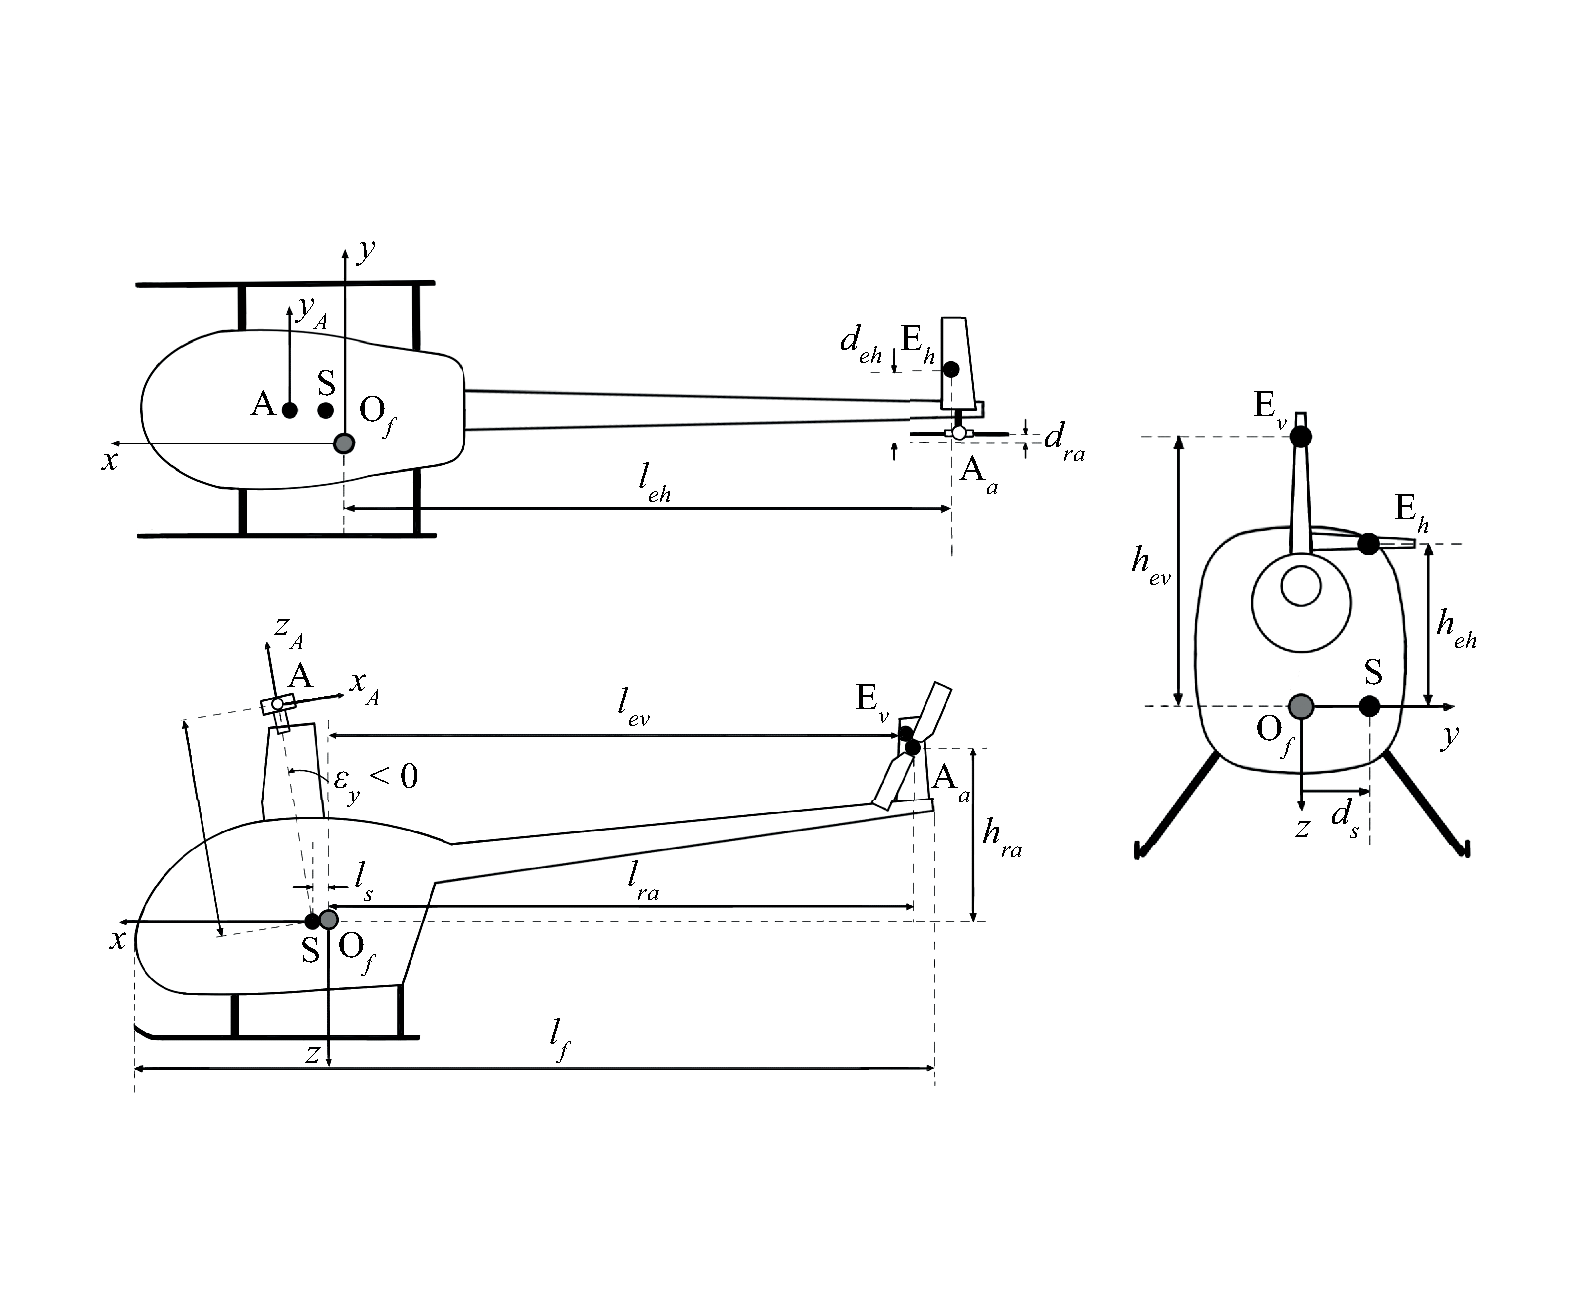
\includegraphics[width=120mm]{imagenes/geometria}
	\caption{Esquema de las medidas indicadas en la tabla \ref{GeBo} sobre las distintas vistas de un helicóptero genérico.}
	\label{GeBodraw}
\end{figure}

\begin{table}[htbp]
	\centering
	\begin{tabular}{|>{\columncolor{Gray}}c|c|}
		\hline
		\cellcolor{Gray}Posición longitudinal del centro de masas respecto a $O_f$ ($x_{CG}$) & 0.1577 m \\ \hline
		\cellcolor{Gray}Posición lateral del centro de masas respecto a $O_f$ ($y_{CG}$) & 0 m \\ \hline
		\cellcolor{Gray}Posición vertical del centro de masas respecto a $O_f$ ($z_{CG}$) & 0 m \\ \hline
		\cellcolor{Gray}Inclinación del eje del árbol respecto al plano $xz$ ($\varepsilon_x$) & 0 rad \\ \hline
		\cellcolor{Gray}Inclinación del eje del árbol respecto al plano $yz$ ($\varepsilon_y$) & -0.523 rad \\ \hline
		\cellcolor{Gray}Componente $x$ del vector $\boldsymbol{O_fS}$ ($l_s$) & 0 m \\ \hline
		\cellcolor{Gray}Componente $y$ del vector $\boldsymbol{O_fS}$ ($d_s$) & 0 m \\ \hline
		\cellcolor{Gray}Longitud del árbol, desde $S$ hasta $A$ ($h$) & 1.48 m \\ \hline
		\cellcolor{Gray}Inclinación del rotor antipar ($\theta_{ra}$) & 0 rad \\ \hline
		\cellcolor{Gray}Componente $x$ del vector $\boldsymbol{O_fA_a}$ ($l_{ra}$) & -5.9226 m \\ \hline
		\cellcolor{Gray}Componente $y$ del vector $\boldsymbol{O_fA_a}$ ($d_{ra}$) & -0.3 m \\ \hline
		\cellcolor{Gray}Componente $z$ del vector $\boldsymbol{O_fA_a}$ ($h_{ra}$) & -1.6426 m \\ \hline
		\cellcolor{Gray}Ángulo de orientación del estabilizador vertical ($\gamma_{ev}$) & $\pi$/2 rad \\ \hline
		\cellcolor{Gray}Componente $x$ del vector $\boldsymbol{O_fE_v}$ ($l_{ev}$) & -5.3386 m \\ \hline
		\cellcolor{Gray}Componente $y$ del vector $\boldsymbol{O_fE_v}$ ($d_{ev}$) & 0 m \\ \hline
		\cellcolor{Gray}Componente $z$ del vector $\boldsymbol{O_fE_v}$ ($h_{ev}$) & -0.86 m \\ \hline
		\cellcolor{Gray}Ángulo de orientación del estabilizador horizontal (dcha.) ($\gamma_{eh,d}$) & 0 rad \\ \hline
		\cellcolor{Gray}Componente $x$ del vector $\boldsymbol{O_fE_h}$ parte dcha. ($l_{eh,d}$) & -4.4826 m \\ \hline
		\cellcolor{Gray}Componente $y$ del vector $\boldsymbol{O_fE_h}$ parte dcha. ($d_{eh,d}$) & 0.969 m \\ \hline
		\cellcolor{Gray}Componente $z$ del vector $\boldsymbol{O_fE_h}$ parte dcha. ($h_{eh,d}$) & 0 m \\ \hline
		\cellcolor{Gray}Ángulo de orientación del estabilizador horizontal (izqda.) ($\gamma_{eh,i}$) & 0 rad \\ \hline
		\cellcolor{Gray}Componente $x$ del vector $\boldsymbol{O_fE_h}$ parte izqda. ($l_{eh,i}$) & -4.4826 m \\ \hline
		\cellcolor{Gray}Componente $y$ del vector $\boldsymbol{O_fE_h}$ parte izqda. ($d_{eh,i}$) & -0.969 m \\ \hline
		\cellcolor{Gray}Componente $z$ del vector $\boldsymbol{O_fE_h}$ parte izqda. ($h_{eh,i}$) & 0 m \\ \hline
	\end{tabular}%
	\caption{Valores de diferentes parámetros geométricos de la aeronave Bölkow Bo 105.}
	\label{GeBo}
\end{table}%

\subsection{Inercia del Bo 105}

Para finalizar con la descripción del modelo del helicóptero, la tabla \ref{InBo} refleja los datos acerca de la inercia del mismo.

\begin{table}[htbp]
	\centering
	\begin{tabular}{|>{\columncolor{Gray}}c|c|}
		\hline
		\cellcolor{Gray}Peso del helicóptero ($W$) & \cellcolor[rgb]{ 1,  1,  1}21560 N \\ \hline
		\cellcolor{Gray}Momento de inercia del eje $x$ ($I_{x}$) & \cellcolor[rgb]{ 1,  1,  1}1433 kg$\cdot$m$^2$ \\ \hline
		\cellcolor{Gray}Momento de inercia del eje $y$ ($I_{y}$) & \cellcolor[rgb]{ 1,  1,  1}4973 kg$\cdot$m$^2$ \\ \hline
		\cellcolor{Gray}Momento de inercia del eje $z$ ($I_{z}$) & \cellcolor[rgb]{ 1,  1,  1}4099 kg$\cdot$m$^2$ \\ \hline
		\cellcolor{Gray}Producto de inercia $xy$ ($I_{xy}$)& \cellcolor[rgb]{ 1,  1,  1}0 kg$\cdot$m$^2$ \\ \hline
		\cellcolor{Gray}Producto de inercia $xz$ ($I_{xz}$)& \cellcolor[rgb]{ 1,  1,  1}660 kg$\cdot$m$^2$ \\ \hline
		\cellcolor{Gray}Producto de inercia $yz$ ($I_{yz}$)& \cellcolor[rgb]{ 1,  1,  1}0 kg$\cdot$m$^2$ \\ \hline
	\end{tabular}%
	\caption{Valores de inercia de la aeronave Bölkow Bo 105.}
	\label{InBo}
\end{table}%

Con este modelo y los parámetros de diseño calculado estadísticamente se generará un modelo inicial que se empleará en las simulaciones para comprobar su desempeño y optimizarlo según las necesidades.

\section{Adimensionalización del Modelo}

Una vez esta definido el helicóptero base, es necesario realizar una adimensionalización del modelo para poder obtener luego un modelo válido para el diseño requerido.

En \citet{Cuerva} se habla de dos posibles adimensionalizaciones en el ámbito de los helicópteros, cada cual con una velocidad característica:

\begin{itemize}
	\item Primera forma adimensional: se emplea la velocidad inducida dada por la teoría de la cantidad de movimiento en vuelo a punto fijo, $v_{i0}$.
	\item Segunda forma adimensional: se emplea la velocidad en punta de pala, $\Omega R$, con $\Omega$ la velocidad de giro del rotor y $R$ el radio del mismo. Usar esta velocidad como velocidad de referencia permite definir magnitudes características de fuerza, par y potencia.
\end{itemize}

Debido a la existencia de parámetros de fuerza, par y potencia en el modelo del Bölkow Bo 105, resulta conveniente emplear la segunda forma adimensional, lo que define las siguientes magnitudes de fuerza, par y potencia:

\begin{itemize}
	\item Tracción unitaria: $T_u=\rho S(\Omega R)^2$, donde $S=\pi R^2$
	\item Par unitario: $Q_u=\rho SR(\Omega R)^2$
	\item Potencia unitaria: $P_u=\rho S(\Omega R)^3$
\end{itemize}

Estas magnitudes permiten a su vez definir los coeficientes de tracción, $C_T=\frac{T}{T_u}$, y de potencia o par, $C_Q=C_P=\frac{Q}{Q_u}=\frac{P}{P_u}$.

Una vez definida la formulación adimensional a usar, solo resta adimensionalizar cada una de las estructuras definidas en el apartado anterior.

\subsection{Rotores Principal y Antipar}

Adimensionalizar los parámetros correspondientes a ambos rotores requiere el uso de magnitudes características de longitud y velocidad, que serán el radio del rotor y la velocidad en punta de pala, pero además el modelo computacional de \emph{HEROES} requerirá de los parámetros atmosféricos a nivel del mar (H=0) de gravedad, $g$, densidad, $\rho$, viscosidad dinámica del fluido y velocidad del sonido.

Al adimensionalizar la estructura del helicóptero base se obtendrán para cada rotor estructuras con los siguientes parámetros:
\singlespacing
\begin{multicols}{2}
	\begin{itemize}
		\item Número de palas: $b$
		\item Solidez del rotor: $\sigma=\frac{c\cdot b}{\pi\cdot R}$
		\item Parámetros de la polar: $\delta_0$, $delta_1$ y $\delta_2$
		\item Coeficiente de sustentación de los perfiles: $c_l$
		\item Torsión lineal de los perfiles: $\theta_1$
		\item Excentricidad adimensional: $e/R$
		\item $\varepsilon_R=\frac{m_b\cdot R\cdot x_{GB}}{I_\beta}$
		\item "Gravedad adimensional"$=\frac{g}{\Omega^2R}$
		\item Rigidez en batimiento adimensional: $K_\beta=\frac{k_\beta}{\rho \pi R^2(\Omega R)^2R}$
		\item Frecuencia natural adimensional no amortiguada en batimiento: $\lambda_\beta=1+\frac{x_{GB}\cdot m_b\cdot e}{I_\beta}+\frac{k_\beta}{I_\beta\cdot\Omega^2}$
		\item Número de Lock: $\gamma=\frac{\rho c_0cR^4}{I_\beta}$
		\item Número de rigidez: $S_\beta=\frac{8(\lambda_\beta^2-1)}{\gamma}$
		\item Relación adimensional $I_\theta/I_\beta$
		\item Relación adimensional $I_\zeta/I_\beta$
		\item Posición adimensional del centro de gravedad de la pala: $X_{GB}=x_{GB}/R$
		\item Parámetro $\mu_p=\frac{m_b}{\rho\pi R^3}$
		\item Número de Reynolds: $Re$
		\item Número de Mach: $M=\frac{\Omega R}{v_{sound}}$
		\end{itemize}
\end{multicols}
\spacing{1.5}
Además de estos parámetros, en la estructura del helicóptero adimensional (la correspondiente al helicóptero completo, no a la de los rotores) aparecerán también los siguientes parámetros:
\singlespacing
\begin{multicols}{2}
	\begin{itemize}
		\item Relación de velocidades angulares: $\frac{\Omega_a}{\Omega}$
		\item Relación de velocidades: $\frac{\Omega_aR_a}{\Omega R}$
		\item Relación de fuerzas $\frac{(\Omega_aR_a)^2R_a^2}{(\Omega R)^2R^3}$
		\item Relación de momentos $\frac{(\Omega_aR_a)^2R_a^2}{(\Omega R)^2R^3}$
	\end{itemize}
\end{multicols}
\spacing{1.5}
\subsection{Fuselaje}

Al estar la estructura del fuselaje compuesta únicamente por características físicas y coeficientes aerodinámicos, solo es necesario definir las adimensionalizaciones para los primeros, pues los segundos ya lo están. Dichas adimensionalizaciones quedarían de la siguiente forma:

\singlespacing
\begin{multicols}{2}
	\begin{itemize}
		\item Longitud del fuselaje: $l_f/R$
		\item Superficie en planta del fuselaje: $\frac{S_s}{\pi R^2}$
		\item Superficie lateral del fuselaje: $\frac{S_l}{\pi R^2}$
	\end{itemize}
\end{multicols}
\spacing{1.5}

Aunque no es un coeficiente aerodinámico, el factor de interferencia del rotor principal con el fuselaje, $k_f$, ya es adimensional por lo que no es necesario trabajarlo.

\subsection{Estabilizadores Vertical y Horizontal}

El caso de los estabilizadores es similar al del fuselaje, únicamente será necesario indicar las adimensionalizaciones de las características físicas ya que el resto son parámetros adimensionales, los cuales quedaría de la siguiente forma:

\singlespacing
\begin{multicols}{2}
	\begin{itemize}
		\item Estabilizador vertical
		\subitem Cuerda del perfil adimensional: $c_{ev}/R$
		\subitem Superficie adimensional: $\frac{S_{ev}}{\pi R^2}$
		\item Estabilizador horizontal
		\subitem Cuerda del perfil adimensional: $c_{eh}/R$
		\subitem Superficie adimensional: $\frac{S_{eh}}{\pi R^2}$
	\end{itemize}
\end{multicols}
\spacing{1.5}

\subsection{Geometría e Inercia del Helicóptero}

En lo que respecta a la geometría, la adimensionalización resulta tan simple como emplear el radio del rotor $R$ para todos los parámetros.

Por otro lado, al adimensionalizar los parámetros de inercia quedarán como se indica a continuación:

\singlespacing
\begin{multicols}{2}
	\begin{itemize}
		\item Coeficiente de peso: $C_w=\frac{W}{T_u}$
		\item Parámetro adimensional $\gamma_x=\frac{\rho\pi R^5}{I_x}$
		\item Parámetro adimensional $\gamma_y=\frac{\rho\pi R^5}{I_y}$
		\item Parámetro adimensional $\gamma_z=\frac{\rho\pi R^5}{I_z}$
		\item Relación adimensional $\frac{I_x}{I_y}$
		\item Relación adimensional $\frac{I_z}{I_y}$
		\item Relación adimensional $\frac{I_{xy}}{I_y}$
		\item Relación adimensional $\frac{I_{xz}}{I_y}$
		\item Relación adimensional $\frac{I_{yz}}{I_y}$
	\end{itemize}
\end{multicols}
\spacing{1.5}

Con todos estos datos y los parámetros de diseño radio del rotor, velocidad de giro de rotor, numero de palas del rotor principal y antipar y peso del nuevo helicóptero, se puede obtener un modelo completo para el nuevo diseño.

\section{Limitaciones a la Velocidad de Giro del Rotor Principal}

Aunque se han calculado estadísticamente los parámetros que definen en una primera aproximación el vehículo a diseñar, debido a la falta de datos de helicópteros existentes similares y a la dispersión de los pocos de los que se dispone suficiente información, es probable que el modelo no resulte realista y no pueda llegar a funcionar correctamente en una situación de vuelo fuera de la simulación. El parámetro del que menos información se dispone es de la velocidad de giro de los rotores de los modelos de las base de datos, por lo que conviene encontrar un valor que pueda resultar mejor. Para ello se ha empleado un concepto físico importante como es el Mach crítico $M_{crit}$ en la punta de pala.

La limitación en la velocidad de giro del rotor viene dada por la aparición de efectos supersónicos en las puntas de las palas del mismo. Estos efectos, como puedan ser ondas de choque, empeoran el comportamiento de las palas, pueden hacerlas entrar en pérdida e incluso provocar daños estructurales debido a cargas elevadas.
Por esto es común establecer un límite conocido como $M_{crit}$ basado en la velocidad $\Omega R$, es decir, la velocidad de avance de las puntas de las palas. Este límite suele ser del orden de 0,4 para vuelo estacionario y 0,8 para vuelo en avance. 
Para poder dar un valor lo más óptimo posible, se ha realizado una simulación de vuelo estacionario de un vehículo con las características obtenidas estadísticamente, a excepción de la velocidad de giro del rotor principal y del radio del mismo, que se han variado para poder obtener el mejor valor posible de estos parámetros.


\begin{figure}
	\centering
	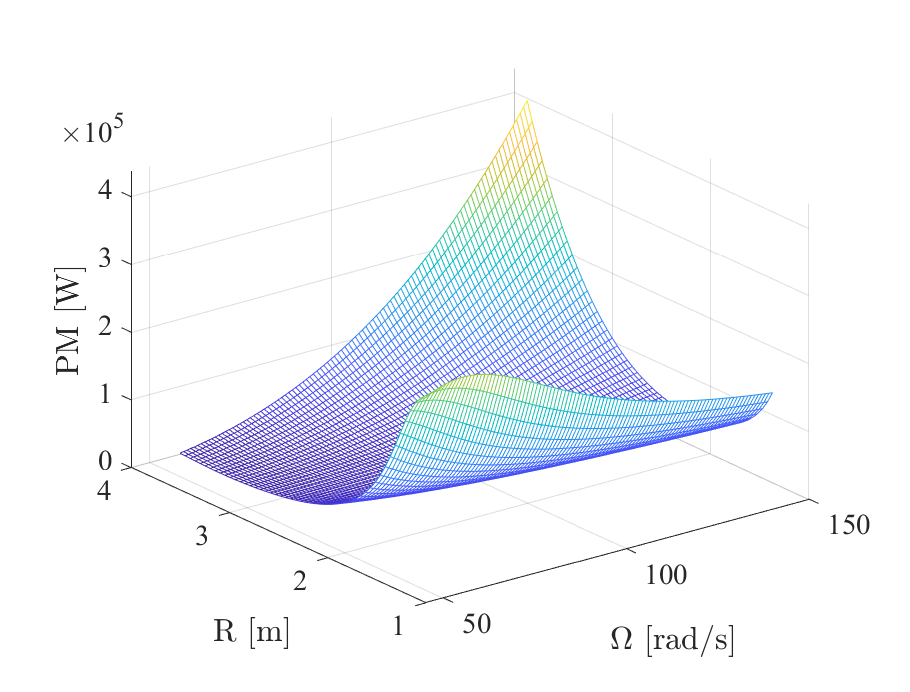
\includegraphics[width=90mm]{graficos/3d3d}
	\caption{Consumo de Potencia de la aeronave en función de la velocidad de giro del rotor y el radio del mismo.}
	\label{ORP}
\end{figure}
\begin{figure}
	\centering
	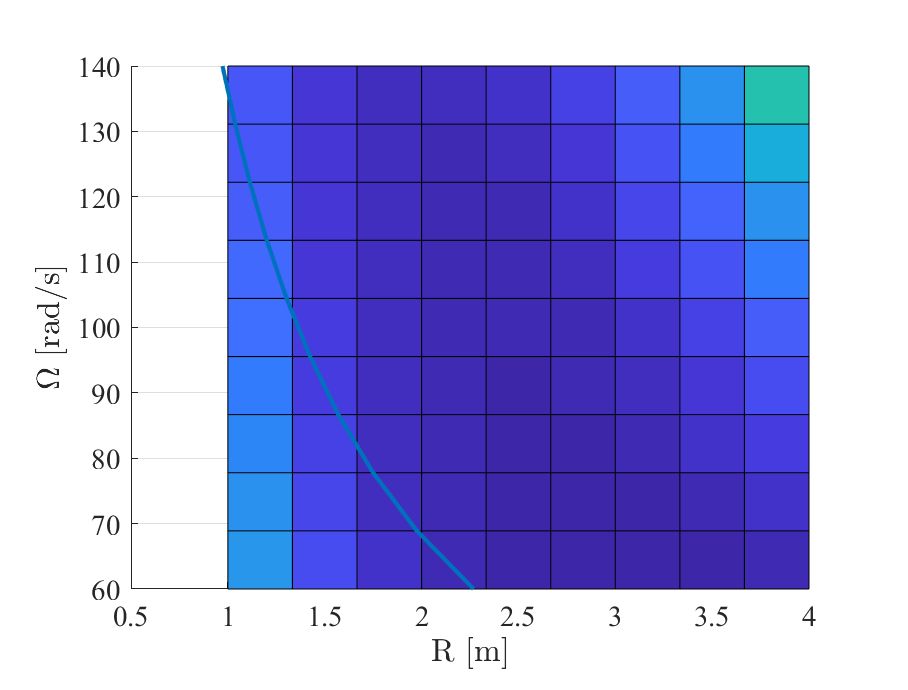
\includegraphics[width=90mm]{graficos/3d2d}
	\caption{Consumo de Potencia de la aeronave en función de la velocidad de giro del rotor y el radio del mismo junto a la línea de las potencias mínimas para cada configuración concreta de $\Omega$ y la limitación de $\Omega$ a causa del $M_{crit}$ (0,4).}
	\label{ORPM}
\end{figure}

La gráfica \ref{ORP} representa la superficie que da un valor de potencia de la aeronave para cada $\Omega$ y $R$ del rotor. Con esto es posible observar los valores mínimos de potencia, lo que nos permite elegir unos valores de $\Omega$ y $R$ que optimicen la potencia necesaria.
Sin embargo, al añadir la limitación del $M_{crit}$ las opciones de configuración disponibles se ven reducidas a aquellas que la cumplan. La gráfica \ref{ORPM} representa la superficie de la gráfica \ref{ORP} sobre el plano $\Omega R$ y encima la anterior limitación junto con una línea que representa las potencias mínimas absolutas para cada configuración de $\Omega$. Aunque estas líneas no se crucen, para los valores más bajos de $\Omega$ se encuentran suficientemente cerca como para pensar que las potencias necesarias son lo suficientemente bajas.
Se observa claramente que los valores de potencia necesaria se reducen con $\Omega$ y con el aumento de radio, por lo que en primera instancia el menor valor dado, quedando automáticamente definido el radio del rotor.

\begin{itemize}
	\item Velocidad de giro del rotor principal $\Omega$ = 45 $rad/s$
	\item Radio del rotor principal $R$ = 3.0248 $m$
\end{itemize}

\section{Obtención del modelo del helicóptero \emph{DroneHE}}

El objetivo es obtener un modelo de helicóptero lo más próximo posible al diseño final sobre el que se puedan realizar unas primeras simulaciones de vuelo para comprobar si es válido y, en caso contrario, modificar el diseño para alcanzar unos resultados mejores. Su obtención se consigue empleando la herramienta \emph{HEROES}, que primero adimensionalizará el helicóptero base ya definido en el capítulo como se ha visto, para después dimensionar un nuevo modelo, al que llamaremos \emph{DroneHE}, usando los parámetros que hemos obtenido. Los resultados se recogen en las tablas \ref{RPHS}, \ref{RaHS}, \ref{FHS}, \ref{EHS}, \ref{GeHs} y \ref{InHS}.
Cabe destacar que se exponen los mismos datos que del Bölkow Bo 105 para poder realizar una comparación rápida de ambos modelos. Además, se han conservado todas las consideraciones hechas a la hora de modelizar el helicóptero base, así como las ecuaciones que permiten calcular los coeficientes adimensionales de fuerzas y momentos aerodinámicos. Los factores de pérdidas en las trasmisiones también se conservan en ambos modelos, siendo estos:

\begin{itemize}
	\item $\eta_{Trp}=0.12$
	\item $\eta_{Tra}=0.07$
\end{itemize}

\begin{table}[]
	\centering
	\begin{tabular}{|>{\columncolor{Gray}}c|c|}
		\hline
		Radio de las palas ($R$) & 3.0248 $m$ \\ \hline
		Excentricidad ($e$) & 0 $m$ \\ \hline
		Número de palas ($b$) & 2 \\ \hline
		Torsión lineal de los perfiles ($\theta_1$) & -0.14 \\ \hline
		Pendiente de la curva de sustentación ($\alpha$) & 6.113 $rad^{-1}$ \\ \hline
		\cellcolor{Gray} & 0.0074 \\ \cline{2-2} 
		\cellcolor{Gray} & 0.0096 $rad^{-1}$ \\ \cline{2-2} 
		\multirow{-3}{*}{\cellcolor{Gray}Parámetros de la polar ($\delta_0$, $\delta_1$, $\delta_2$)} & 0.294 $rad^{-2}$ \\ \hline
		Velocidad de giro del rotor ($\Omega$) & 45 $rad/s$ \\ \hline
		Cuerda del perfil ($c$) & 0.3327 $m$ \\ \hline
		Momento de inercia de la pala en batimiento ($I_\beta$) & 41.1204 $kgm^2$ \\ \hline
		Momento de inercia de la pala en paso ($I_\theta$) & 01.2423 $kgm^2$ \\ \hline
		Momento de inercia de la pala en arrastre ($I_\zeta$) & 42.3627 $kgm^2$ \\ \hline
		Posición del centro de gravedad de la pala ($x_{GB}$) & 1.5063 $m$ \\ \hline
		Masa de la pala ($m_b$) & 18.7982 $kg$ \\ \hline
		Rigidez en batimiento ($k_\beta$) & 10330 $Nm/rad$ \\ \hline
	\end{tabular}
	\caption{Valores de diferentes parámetros del rotor principal del \emph{DroneHE}.}
	\label{RPHS}
\end{table}

\begin{table}[htbp]
	\centering
	\begin{tabular}{|>{\columncolor{Gray}}c|c|}
		\hline
		Radio de las palas ($R$) & 0.5853 $m$ \\ \hline
		Excentricidad ($e$) & 0 $m$ \\ \hline
		Número de palas ($b$) & 2 \\ \hline
		Torsión lineal de los perfiles ($\theta_1$) & \cellcolor[rgb]{ 1,  1,  1}0 \\ \hline
		Pendiente de la curva de sustentación ($\alpha$) & 5.7 $rad^{-1}$ \\ \hline
		\cellcolor{Gray} & 0.008 \\ \cline{2-2}
		\cellcolor{Gray} & 0.0096 $rad^{-1}$ \\ \cline{2-2}
		\multirow{-3}{*}{\cellcolor{Gray}Parámetros de la polar ($\delta_0$, $\delta_1$, $\delta_2$)} & 0.294 $rad^{-2}$ \\ \hline
		Velocidad de giro del rotor ($\Omega$) & \cellcolor[rgb]{ 1,  1,  1}235.6194 $rad/s$ \\ \hline
		Cuerda del perfil ($c$) & \cellcolor[rgb]{ 1,  1,  1}0.1109 $m$ \\ \hline
		Momento de inercia de la pala en batimiento ($I_\beta$) & 0.1602 $kgm^2$ \\ \hline
		Momento de inercia de la pala en paso ($I_\theta$) & 0.0058 $kgm^2$ \\ \hline
		Momento de inercia de la pala en arrastre ($I_\zeta$) & 0.1659 $kgm^2$ \\ \hline
		Posición del centro de gravedad de la pala ($X_{GB}$) & 0.2926 $m$ \\ \hline
		Masa de la pala ($m_b$) & 1.4029 $kg$ \\ \hline
		\cellcolor{Gray}Rigidez en batimiento ($I_\beta$) & $9.1151^{98}$ $Nm/rad$ \\ \hline
	\end{tabular}%
	\caption{Valores de diferentes parámetros del rotor antipar del \emph{DroneHE}.}
	\label{RaHS}
\end{table}%

\begin{table}[htbp]
	\centering
	\begin{tabular}{|>{\columncolor{Gray}}c|c|}
		\hline
		\cellcolor{Gray}Longitud del fuselaje ($l_f$) & \cellcolor[rgb]{ 1,  1,  1}5.2734 $m$ \\ \hline
		\cellcolor{Gray}Superficie en planta del fuselaje ($S_p$)& \cellcolor[rgb]{ 1,  1,  1}2.8464 $m^2$ \\ \hline
		\cellcolor{Gray}Superficie lateral del fuselaje ($S_l$) & \cellcolor[rgb]{ 1,  1,  1}3.1501 \\ \hline
		\cellcolor{Gray}Factor de interferencia del rotor principal sobre el fuselaje ($k_f$) & \cellcolor[rgb]{ 1,  1,  1}1 \\ \hline
	\end{tabular}%
	\caption{Valores de los parámetros del fuselaje del \emph{DroneHE}.}
	\label{FHS}
\end{table}%

\begin{table}[htbp]
	\centering
	\begin{tabular}{|>{\columncolor{Gray}}c|c|}
		\hline
		\cellcolor{Gray}Cuerda del estabilizador vertical ($c_{ev}$) & \cellcolor[rgb]{ 1,  1,  1}0.1848 $m$ \\ \hline
		\cellcolor{Gray}Superficie del estabilizador vertical ($S_{ev}$)& \cellcolor[rgb]{ 1,  1,  1}0.3055 $m^2$ \\ \hline
		\cellcolor{Gray}Ángulo de calado del estabilizador vertical ($\theta_{ev}$) & \cellcolor[rgb]{ 1,  1,  1}0.0812 $rad$ \\ \hline
		\cellcolor{Gray}Cuerda del estabilizador horizontal ($c_{ev}$) & \cellcolor[rgb]{ 1,  1,  1}0.2464 $m$ \\ \hline
		\cellcolor{Gray}Superficie del estabilizador horizontal/2 ($S_{ev}$)& \cellcolor[rgb]{ 1,  1,  1}0.1524 $m^2$ \\ \hline
		\cellcolor{Gray}Ángulo de calado del estabilizador horizontal ($\theta_{ev}$) & \cellcolor[rgb]{ 1,  1,  1}0.0698 $rad$ \\ \hline
	\end{tabular}%
	\caption{Valores de diferentes parámetros de los estabilizadores vertical y horizontal del \emph{DroneHE}. La superficie del estabilizador horizontal corresponde a la mitad ya que el mismo esta dividido en 2 partes al haber usado como base el Bölkow Bo 105.}
	\label{EHS}
\end{table}%

\begin{table}[htbp]
	\centering
	\begin{tabular}{|>{\columncolor{Gray}}c|c|}
		\hline
		\cellcolor{Gray}Posición longitudinal del centro de masas respecto a $O_f$ ($x_{CG}$) & 0.0972 m \\ \hline
		\cellcolor{Gray}Posición lateral del centro de masas respecto a $O_f$ ($y_{CG}$) & 0 m \\ \hline
		\cellcolor{Gray}Posición vertical del centro de masas respecto a $O_f$ ($z_{CG}$) & 0 m \\ \hline
		\cellcolor{Gray}Inclinación del eje del árbol respecto al plano $xz$ ($\varepsilon_x$) & 0 rad \\ \hline
		\cellcolor{Gray}Inclinación del eje del árbol respecto al plano $yz$ ($\varepsilon_y$) & -0.523 rad \\ \hline
		\cellcolor{Gray}Componente $x$ del vector $\boldsymbol{O_fS}$ ($l_s$) & 0 m \\ \hline
		\cellcolor{Gray}Componente $y$ del vector $\boldsymbol{O_fS}$ ($d_s$) & 0 m \\ \hline
		\cellcolor{Gray}Longitud del árbol, desde $S$ hasta $A$ ($h$) & 0.9118 m \\ \hline
		\cellcolor{Gray}Inclinación del rotor antipar ($\theta_{ra}$) & 0 rad \\ \hline
		\cellcolor{Gray}Componente $x$ del vector $\boldsymbol{O_fA_a}$ ($l_{ra}$) & -3.6487 m \\ \hline
		\cellcolor{Gray}Componente $y$ del vector $\boldsymbol{O_fA_a}$ ($d_{ra}$) & -0.1848 m \\ \hline
		\cellcolor{Gray}Componente $z$ del vector $\boldsymbol{O_fA_a}$ ($h_{ra}$) & -1.0596 m \\ \hline
		\cellcolor{Gray}Ángulo de orientación del estabilizador vertical ($\gamma_{ev}$) & $\pi$/2 rad \\ \hline
		\cellcolor{Gray}Componente $x$ del vector $\boldsymbol{O_fE_v}$ ($l_{ev}$) & -3.2889 m \\ \hline
		\cellcolor{Gray}Componente $y$ del vector $\boldsymbol{O_fE_v}$ ($d_{ev}$) & 0 m \\ \hline
		\cellcolor{Gray}Componente $z$ del vector $\boldsymbol{O_fE_v}$ ($h_{ev}$) & -0.5298 m \\ \hline
		\cellcolor{Gray}Ángulo de orientación del estabilizador horizontal (dcha.) ($\gamma_{eh,d}$) & 0 rad \\ \hline
		\cellcolor{Gray}Componente $x$ del vector $\boldsymbol{O_fE_h}$ parte dcha. ($l_{eh,d}$) & -2.7615 m \\ \hline
		\cellcolor{Gray}Componente $y$ del vector $\boldsymbol{O_fE_h}$ parte dcha. ($d_{eh,d}$) & 0.597 m \\ \hline
		\cellcolor{Gray}Componente $z$ del vector $\boldsymbol{O_fE_h}$ parte dcha. ($h_{eh,d}$) & 0 m \\ \hline
		\cellcolor{Gray}Ángulo de orientación del estabilizador horizontal (izqda.) ($\gamma_{eh,i}$) & 0 rad \\ \hline
		\cellcolor{Gray}Componente $x$ del vector $\boldsymbol{O_fE_h}$ parte izqda. ($l_{eh,i}$) & -2.7615 m \\ \hline
		\cellcolor{Gray}Componente $y$ del vector $\boldsymbol{O_fE_h}$ parte izqda. ($d_{eh,i}$) & -0.597 m \\ \hline
		\cellcolor{Gray}Componente $z$ del vector $\boldsymbol{O_fE_h}$ parte izqda. ($h_{eh,i}$) & 0 m \\ \hline
	\end{tabular}%
	\caption{Valores de diferentes parámetros geométricos del \emph{DroneHE}.}
	\label{GeHs}
\end{table}%

\begin{table}[htbp]
	\centering
	\begin{tabular}{|>{\columncolor{Gray}}c|c|}
		\hline
		\cellcolor{Gray}Peso del helicóptero ($W$) & \cellcolor[rgb]{ 1,  1,  1}4413 $N$ \\ \hline
		\cellcolor{Gray}Momento de inercia del eje $x$ ($I_{x}$) & \cellcolor[rgb]{ 1,  1,  1}127.1591 $kg\cdot m^2$ \\ \hline
		\cellcolor{Gray}Momento de inercia del eje $y$ ($I_{y}$) & \cellcolor[rgb]{ 1,  1,  1}441.2856 $kg\cdot m^2$ \\ \hline
		\cellcolor{Gray}Momento de inercia del eje $z$ ($I_{z}$) & \cellcolor[rgb]{ 1,  1,  1}363.7301 $kg\cdot m^2$ \\ \hline
		\cellcolor{Gray}Producto de inercia $xy$ ($I_{xy}$)& \cellcolor[rgb]{ 1,  1,  1}0 $kg\cdot m^2$ \\ \hline
		\cellcolor{Gray}Producto de inercia $xz$ ($I_{xz}$)& \cellcolor[rgb]{ 1,  1,  1}58.566 $kg\cdot m^2$ \\ \hline
		\cellcolor{Gray}Producto de inercia $yz$ ($I_{yz}$)& \cellcolor[rgb]{ 1,  1,  1}0 $kg\cdot m^2$ \\ \hline
	\end{tabular}%
	\caption{Valores de inercia del \emph{DroneHE}.}
	\label{InHS}
\end{table}%

Se observa claramente en los resultados que el proceso de generación del modelo del helicóptero semilla ha sido correcto, estando todas sus magnitudes dimensionalizadas acorde a los requisitos de diseño, especialmente la masa y el tamaño, que son significativamente diferentes al helicóptero base.
También se observa que hay parámetros que se han mantenido iguales en ambos diseños. Estos parámetros son, por ejemplo, los ángulos de calado de las palas o la pendiente de la curva de sustentación de las palas. Todas estas características son los parámetros adimensionales de diseño, y no dependen del tamaño del vehículo sino de elecciones de diseño como puedan ser los perfiles que se utilicen en las palas del rotor.

\section{Modelización de la Carga de Pago}

La modelización realizada al DroneHE supone que la totalidad de equipos necesarios para el vuelo, incluyendo ordenadores y sistemas de comunicación e incluso combustible, ya están embarcados, pero aún falta la carga de pago, que en un helicóptero de vigilancia será una cámara o un sistema de cámaras.

Los dispositivos de vigilancia suelen ir situados en la parte externa del fuselaje, en el suelo del mismo, lo que hace necesario un análisis aerodinámico del mismo para poder realizar una correcta aproximación de las consecuencias reales de montar dicho sistema. Sin embargo, no se disponen de datos suficientes para hacer dichos cálculos, por lo que se optará por una modelización más sencilla que consista únicamente en una variación másica y de inercia del modelo. 

Lo primero es seleccionar el equipo a embarcar, y para ello se presentan varias opciones:

\subsubsection*{Trakka Systems SWE-200 LE}

\noindent\begin{minipage}{0.3\textwidth}% adapt widths of minipages to your needs
	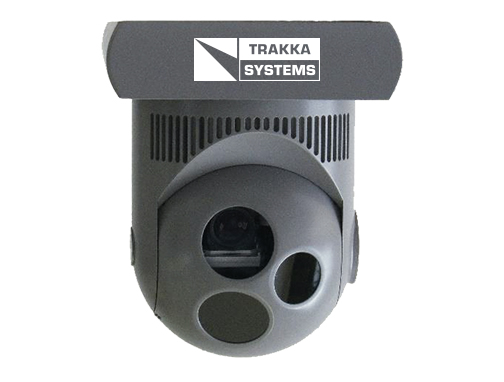
\includegraphics[width=\linewidth]{imagenes/200-LE}
\end{minipage}%
\hfill%
\begin{minipage}{0.7\textwidth}
Especificaciones técnicas
	\begin{itemize}
		\item Diámetro: 200 mm
		\item Peso: 8 kg
		\item Requerimientos de potencia: 22-30 VDC, 250 W
	\end{itemize}
\end{minipage}

\subsubsection*{Trakka Systems TC-300}

\noindent\begin{minipage}{0.3\textwidth}% adapt widths of minipages to your needs
	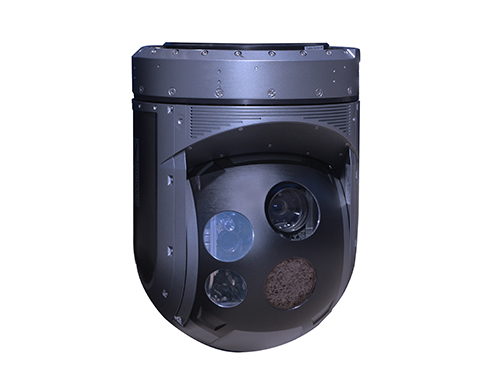
\includegraphics[width=\linewidth]{imagenes/TC-300}
\end{minipage}%
\hfill%
\begin{minipage}{0.7\textwidth}
	Especificaciones técnicas
	\begin{itemize}
		\item Diámetro: 300 mm
		\item Peso: 19 kg
		\item Requerimientos de potencia: 22-36 V, 100-320 W
	\end{itemize}
\end{minipage}

\subsubsection*{Trakka Systems SWE-400 LE}

\noindent\begin{minipage}{0.3\textwidth}% adapt widths of minipages to your needs
	\includegraphics[width=\linewidth]{imagenes/400-le}
\end{minipage}%
\hfill%
\begin{minipage}{0.7\textwidth}
	Especificaciones técnicas
	\begin{itemize}
		\item Diámetro: 400 mm
		\item Peso: 30 kg
		\item Requerimientos de potencia: 22-30VDC, 250 W
	\end{itemize}
\end{minipage}

Estos son solo algunos ejemplos de los sistemas existentes que muestran la enorme variedad de estos, tanto en tamaño y peso como en especificaciones, aunque estas últimas no son objeto de estudio.

Con estos datos se pueden modelizar diferentes cargas que permitan simular diversas condiciones, en el trabajo se emplearán  unas esferas de masa y radio los siguientes:

\begin{itemize}
	\item Carga 1: Masa de 10 kg y radio de 100 mm
	\item Carga 2: Masa de 20 kg y radio de 150 mm
	\item Carga 3: Masa de 30 kg y radio de 200 mm
\end{itemize}

En la tabla \ref{tablaPL} se recogen las características másicas y de inercia de las cargas que han de implementarse en el helicóptero.

\begin{table}[htbp]
	\centering
	\begin{tabular}{|>{\columncolor{Gray}}c|c|}
		\hline
		\cellcolor{Gray}Masa del dispositivo ($M_{pl}$) & 10/20/30 kg \\ \hline
		\cellcolor{Gray}Radio del dispositivo ($R_{pl}$) & 0.1/0.15/0.2 m \\ \hline
		\cellcolor{Gray}Momento de inercia del eje $x$ ($I_{x}^{pl0}$) & 0.04/0.18/0.48 kg$\cdot$m$^2$ \\ \hline
		\cellcolor{Gray}Momento de inercia del eje $y$ ($I_{y}^{pl0}$) & 0.04/0.18/0.48 kg$\cdot$m$^2$ \\ \hline
		\cellcolor{Gray}Momento de inercia del eje $z$ ($I_{z}^{pl0}$) & 0.04/0.18/0.48 kg$\cdot$m$^2$ \\ \hline
		\cellcolor{Gray}Producto de inercia $xy$ ($I_{xy}^{pl0}$)& 0 kg$\cdot$m$^2$ \\ \hline
		\cellcolor{Gray}Producto de inercia $xz$ ($I_{xz}^{pl0}$)& 0 kg$\cdot$m$^2$ \\ \hline
		\cellcolor{Gray}Producto de inercia $yz$ ($I_{yz}^{pl0}$)& 0 kg$\cdot$m$^2$ \\ \hline
		\cellcolor{Gray}Peso del dispositivo ($W_{pl}$)& 10/20/30$\cdot$9.81 N \\ \hline
	\end{tabular}%
	\caption{Valores másicos y de inercia de las diversas cargas de pago que se implementarán en la aeronave.}
	\label{tablaPL}
\end{table}%

\section{Integración de la Carga de Pago}

A la hora de integrar la carga de pago, es muy importante conocer la posición de la misma respecto al centro de masas del helicóptero. Para comprobar que posición puede resultar más favorable, en la tabla \ref{CGPL} se indica un rango de posiciones que se comprobarán en simulaciones posteriores para hallar una posición optima. La posición según el eje $z$ será fija ya que se situará en el suelo del fuselaje en todo momento.

\begin{table}[htbp]
	\centering
	\begin{tabular}{|>{\columncolor{Gray}}c|c|}
		\hline
		\cellcolor{Gray}Posición longitudinal de la carga de pago respecto a $O_f$ ($l_x$) & [-0.65 1.35] m \\ \hline
		\cellcolor{Gray}Posición transversal de la carga de pago respecto a $O_f$ ($l_y$) & [-0.35 0.35] m \\ \hline
		\cellcolor{Gray}Posición vertical del suelo del fuselaje ($l_z$) & 0.6678/0.7178/0.7678 m \\ \hline
	\end{tabular}%
	\caption{Posición de la carga de pago en el fuselaje.}
	\label{CGPL}
\end{table}%

\subsubsection*{Inercia del helicóptero con la carga de pago integrada}

En lo que resta de capítulo, el hiperíndice \emph{$he0$} indicará que se trata de un parámetro del helicóptero en configuración limpia, sin la carga de pago añadida.

Lo primero para poder integrar la carga de pago en la estructura es calcular el nuevo centro de gravedad de la aeronave una vez se ha acoplado la carga de pago. Para ello se pueden usar las siguientes ecuaciones:

\begin{equation}
	X_{CG}^{he}=\frac{x_{CG}^{he0}\cdot W+l_x\cdot W_{pl}}{W+W_{pl}}
\end{equation}
\begin{equation}
	Y_{CG}^{he}=\frac{y_{CG}^{he0}\cdot W+l_y\cdot W_{pl}}{W+W_{pl}}
\end{equation}
\begin{equation}
	Z_{CG}^{he}=\frac{z_{CG}^{he0}\cdot W+l_z\cdot W_{pl}}{W+W_{pl}}
\end{equation}

Una vez posicionado el centro de gravedad del helicóptero, se procede al cálculo de los nuevos valores de inercia de la carga de pago respecto a este centro de masas:

\begin{equation}
I_x^{pl}=I_x^{pl0}+M_{pl}\cdot[(l_y-Y_{CG}^{he})^2+(l_z-Z_{CG}^{he})^2]
\end{equation}
\begin{equation}
I_y^{pl}=I_y^{pl0}+M_{pl}\cdot[(l_x-X_{CG}^{he})^2+(l_z-Z_{CG}^{he})^2]
\end{equation}
\begin{equation}
I_z^{pl}=I_z^{pl0}+M_{pl}\cdot[(l_x-X_{CG}^{he})^2+(l_y-Y_{CG}^{he})^2]
\end{equation}
\begin{equation}
I_x^{pl}=I_x^{pl0}+M_{pl}\cdot(l_y-Y_{CG}^{he})\cdot(l_z-Z_{CG}^{he})
\end{equation}
\begin{equation}
I_y^{pl}=I_y^{pl0}+M_{pl}\cdot(l_x-X_{CG}^{he})\cdot(l_z-Z_{CG}^{he})
\end{equation}
\begin{equation}
I_z^{pl}=I_z^{pl0}+M_{pl}\cdot(l_x-X_{CG}^{he})\cdot(l_y-Y_{CG}^{he})
\end{equation}

El último paso para la integración de la carga de pago consiste en el calculo del tensor de inercia del helicóptero respecto al nuevo centro de gravedad, que se puede calcular con las ecuaciones siguientes:

\begin{equation}
I_x^{he}=I_x^{he0}+M_{pl}\cdot[(y_{CG}^{he0}-Y_{CG}^{he})^2+(z_{CG}^{he0}-Z_{CG}^{he})^2]
\end{equation}
\begin{equation}
I_y^{he}=I_y^{he0}+M_{pl}\cdot[(x_{CG}^{he0}-X_{CG}^{he})^2+(z_{CG}^{he0}-Z_{CG}^{he})^2]
\end{equation}
\begin{equation}
I_z^{he}=I_z^{he0}+M_{pl}\cdot[(x_{CG}^{he0}-X_{CG}^{he})^2+(y_{CG}^{he0}-Y_{CG}^{he})^2]
\end{equation}
\begin{equation}
I_{xy}^{he}=I_{xy}^{he0}+M_{pl}\cdot(x_{CG}^{he0}-X_{CG}^{he})\cdot(y_{CG}^{he0}-Y_{CG}^{he})
\end{equation}
\begin{equation}
I_{xz}^{he}=I_{xx}^{he0}+M_{pl}\cdot(x_{CG}^{he0}-X_{CG}^{he})\cdot(z_{CG}^{he0}-Z_{CG}^{he})
\end{equation}
\begin{equation}
I_{yz}^{he}=I_{yz}^{he0}+M_{pl}\cdot(y_{CG}^{he0}-Y_{CG}^{he})\cdot(z_{CG}^{he0}-Z_{CG}^{he})
\end{equation}

Con estos cálculos ya se han definido todos los parámetros necesarios para poder estudiar el problema del equilibrado del helicóptero con y sin carga de pago, lo que permite realizar las simulaciones de vuelo que se encontrarán en capítulos posteriores de este trabajo.

\singlespacing

\thispagestyle{empty}
\definecolor{Gray2}{rgb}{ .851,  .851,  .851}
\chapter{Vuelo Horizontal}

\spacing{1.5}

Las condiciones para el vuelo rectilíneo son sencillas: la velocidad vertical ha de ser nula, mientras que la horizontal no. Con estas condiciones y a nivel del mar se pueden obtener las gráficas \ref{PMVH}, \ref{ControlVH}, \ref{EulerVH} y \ref{PVH}, que ofrecen una primera aproximación del rendimiento de la aeronave en configuración sin carga de pago. De ellas se puede deducir que el valor de potencia total mínimo es de 27,307 kW, y se da para una velocidad de vuelo de 28.73 m/s. Para calcular la velocidad máxima de avance es necesario obtener características del motor, el cual no se ha decidido, por lo que, para tener unos valores orientativos, se ha optado por emplear los datos del motor que monta el Cicaré 7B, un helicóptero de peso similar al vehículo a diseñar. El motor en cuestión es el ROTAX 912 ULS, un motor de 4 tiempos y 4 cilindros, con un consumo especifico de 285 g/kW$\cdot$ h a una potencia máxima continua de 58 kW a 5500 rpm \citep{ROTAX}. Con esta limitación reflejada en la gráfica \ref{PMVH} se puede observar que el motor, cuya potencia máxima continua disponible es de 58 kW, permite volar a velocidades de hasta casi 70 m/s en estas condiciones.

\begin{figure}
	\centering
	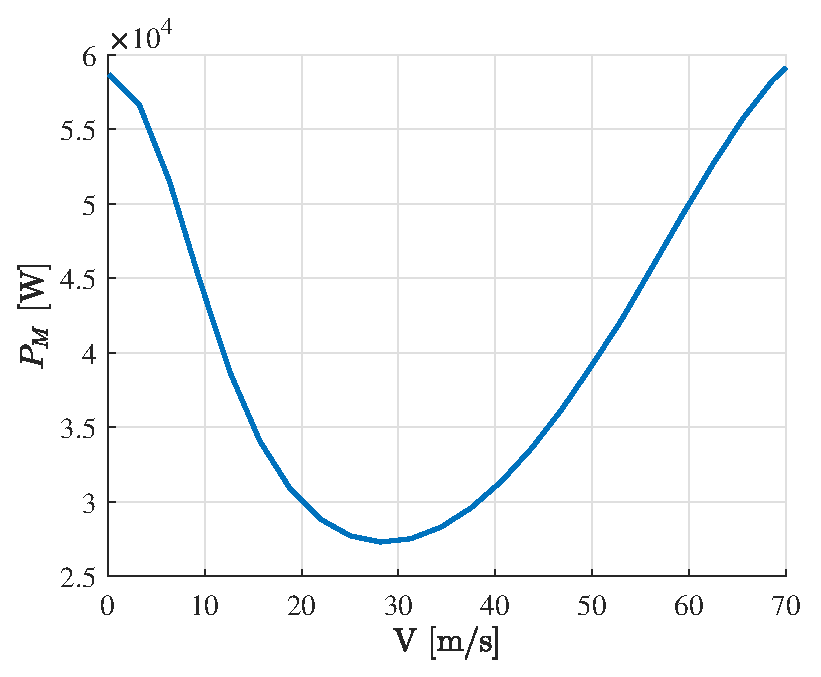
\includegraphics[width=90mm]{graficos/PMVH}
	\caption{Consumo de Potencia de la aeronave en función de la velocidad de vuelo a nivel del mar para vuelo horizontal y limitación por potencia máxima continua disponible.}
	\label{PMVH}
\end{figure}
\begin{figure}
	\centering
	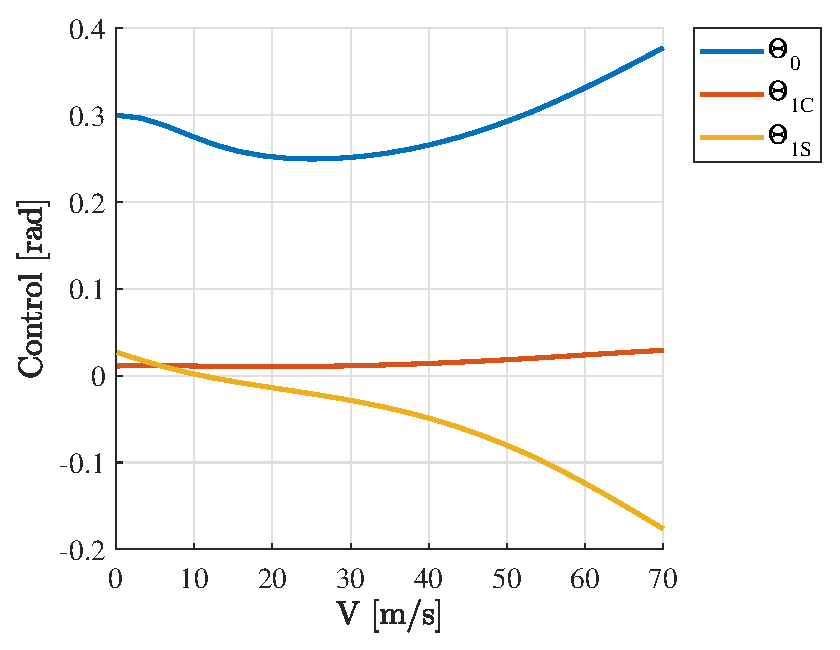
\includegraphics[width=90mm]{graficos/ControlVH}
	\caption{Ángulos de control de la aeronave en función de la velocidad de vuelo a nivel del mar para vuelo horizontal.}
	\label{ControlVH}
\end{figure}
\begin{figure}
	\centering
	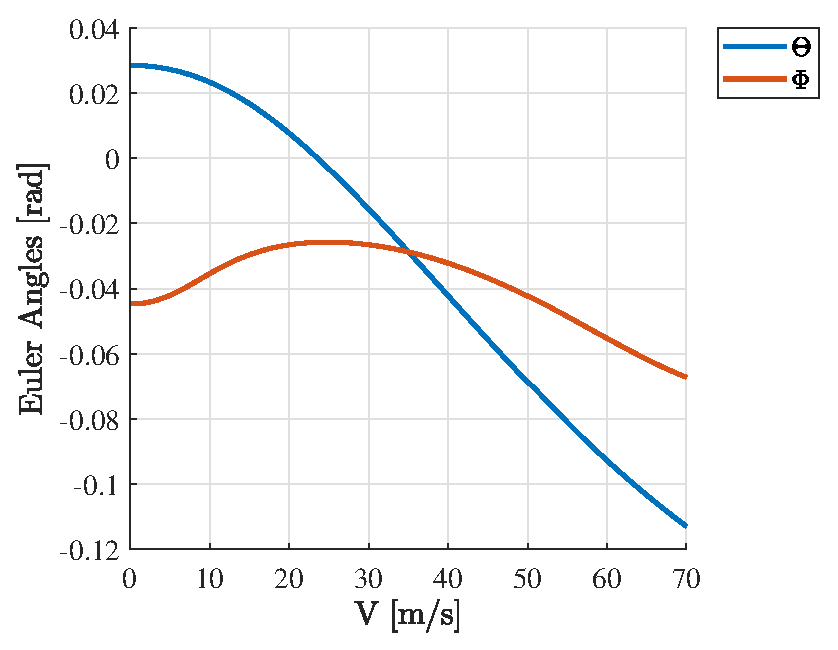
\includegraphics[width=90mm]{graficos/EulerVH}
	\caption{Ángulos de Euler de la aeronave en función de la velocidad de vuelo a nivel del mar para vuelo horizontal.}
	\label{EulerVH}
\end{figure}
\begin{figure}
	\centering
	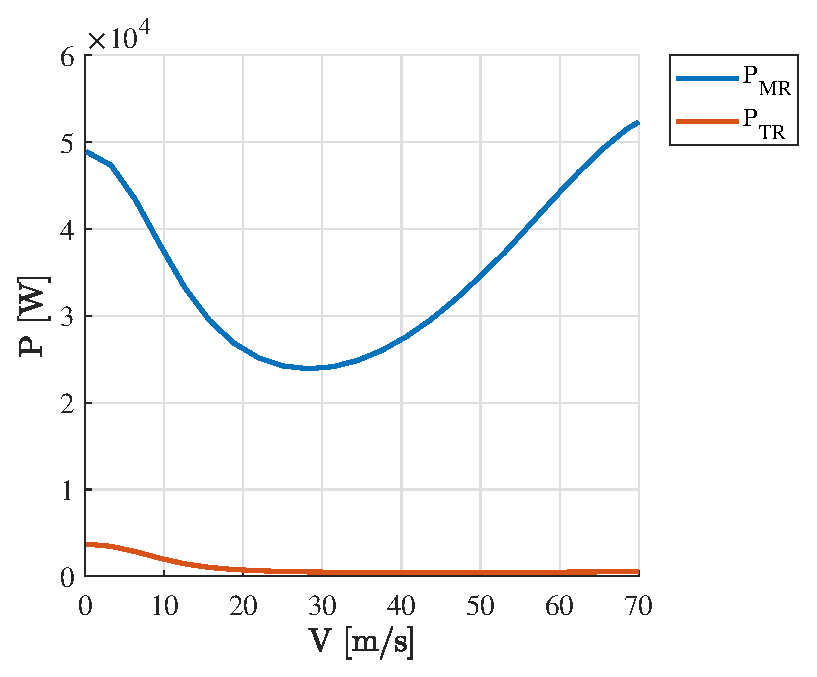
\includegraphics[width=90mm]{graficos/PVH}
	\caption{Consumo de Potencia de los rotores principal y antipar en función de la velocidad de vuelo a nivel del mar para vuelo horizontal.}
	\label{PVH}
\end{figure}

\section{Autonomía de Vuelo}

Con estos datos se puede hacer una estimación de la autonomía del vehículo. 
Para poder obtener el consumo específico del motor en las condiciones de vuelo de máxima autonomía, se emplea el modelo recogido en \citet{Cuerva}, que calcula el consumo en función de la potencia necesaria para el vuelo.
\begin{equation}
	c_e(P)=\frac{c_{e,P_{max}}}{1+\frac{K_m}{c_{e,P_{max}}}(1-\frac{P_{max}}{P(t)})}
	\label{consumo}
\end{equation}
Donde $c_e$ es el consumo específico al régimen de vuelo considerado, $c_{e,P_{max}}$ el consumo específico del motor en régimen de funcionamiento de máxima potencia, $P_{max}$ la potencia máxima continua capaz de ofrecer el motor y $P$ la potencia necesaria para el vuelo considerado.
$K_m$ es un parámetro que mide la eficiencia del motor, que en motores muy eficientes es del orden de 8.33$\cdot$10$^-9$ kg/W$\cdot$s (0.03 kg/kW$\cdot$h).
Además se suponen unas cargas de combustible del 9\% del MTOW del vehículo. 

Lo siguiente es decidir un modelo de cálculo de la autonomía, ya que no se dispone de datos suficientes para hacer unos cálculos exactos,ni estos son necesarios en una fase de diseño preliminar. La hipótesis básica es considerar las masa del vehículo constante durante el vuelo, cosa que no es así por el consumo del propio combustible, pero simplificará los cálculos en gran medida.
Para los cálculos se empleará el método del equilibrado del helicóptero, que permite incluir gran cantidad de información en los cálculos y por tanto aumentar la fiabilidad de estos. Como se desarrollará a continuación, la complejidad de este método reside en el propio equilibrado del helicóptero, que permitirá obtener el valor de potencia requerido para el vuelo, a partir del cual el cálculo de la autonomía resulta trivial.

En \citet{Filippone} se expone un método para calcular la autonomía de forma sencilla empleando para ello la potencia (calculada mediante el equilibrado) del vuelo y el consumo específico (calculado mediante la ecuación \ref{autonomia}).
Se define la autonomía específica $E_s$
\begin{equation}
	E_s=\frac{\partial t}{\partial m}=\frac{1}{\dot{m_f}}=\frac{1}{P\cdot c_{e}(P)}
	\label{autespecifica}
\end{equation}
y con la hipótesis de masa constante solo es necesario resolver el equilibrado para una velocidad ya que
\begin{equation}
	\frac{\partial P}{\partial t}=0\rightarrow P=cte
\end{equation}
que al introducir en la ecuación \ref{consumo} se obtiene que
\begin{equation}
	P=cte\rightarrow c_e=cte
\end{equation}
y por tanto
\begin{equation}
E_s=\frac{1}{P\cdot c_{e}}=cte
\label{autespecificacte}
\end{equation}
Una vez obtenido el valor de la autonomía especifica, el calculo de la autonomía resulta sencillo
\begin{equation}
	t_{e}=E_s\cdot \Delta m=E_s\cdot MFM=\frac{MFM}{c_e\cdot P}
	\label{autonomia}
\end{equation}

Donde $t_e$ es la autonomía, $MFM$ es la masa máxima de combustible, $C_{e}$ es el consumo específico y $P_e$ la potencia en el régimen de de vuelo.
La tabla \ref{auttabla} recoge los datos necesarios para el cálculo de la autonomía máxima y el valor de esta.

\begin{table}[htbp]
	\centering
	\begin{tabular}{|>{\columncolor{Gray}}c|c|}
		\hline
		\cellcolor{Gray2}Variable & \cellcolor{Gray2}Valor \\ \hline \hline
		\cellcolor{Gray}Potencia para máxima autonomía ($P_{min,t_{e,max}}$)  & 27.307 kW \\ \hline
		\cellcolor{Gray}Velocidad en régimen de máxima autonomía ($V$) & 28.73 m/s \\ \hline
		\cellcolor{Gray}Consumo específico en régimen de máxima autonomía ($c_{e,t_{e,max}}$) & 8.98$\cdot$10$^-08$ kg/W$\cdot$s \\ \hline
		\cellcolor{Gray}Máxima autonomía ($t_{e,max}$) & 4.588 h \\ \hline
	\end{tabular}%
	\caption{Valores de inercia del helicóptero semilla.}
	\label{auttabla}
\end{table}%

A modo de comprobación, se han calculado las autonomías correspondientes a distintas velocidades de vuelo en la gráfica \ref{teVH}. Se puede observar que su forma resulta muy similar a la de la gráfica \ref{PMVH} pero invirtiéndola según el eje x. Esto se debe a que la autonomía no depende de otro parámetro de vuelo que no sea la potencia consumida, por lo que la evolución de la potencia necesaria será inversa a la evolución de la autonomía de vuelo, siendo el mínimo de potencia necesaria el máximo de autonomía.

\begin{figure}
	\centering
	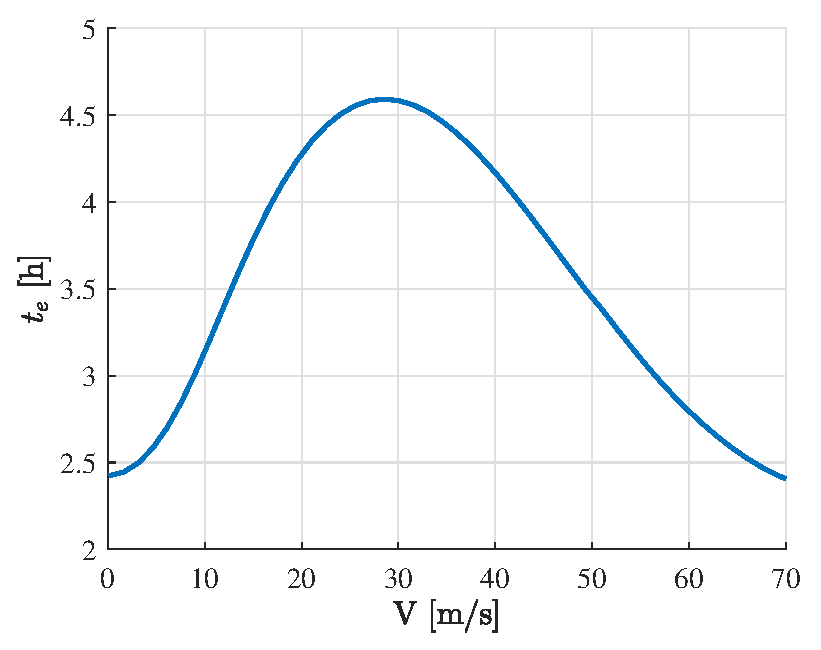
\includegraphics[width=90mm]{graficos/teVH}
	\caption{Autonomía de la aeronave en función de la velocidad de vuelo a nivel del mar para vuelo horizontal.}
	\label{teVH}
\end{figure}
%Los datos del motor son
%Pot. Max. Coontinua 58 Kw
%consumo l/h 22,6 (100%) y 16,2 (75%)
%consumo especifico al 100% 285g/kWh
%Con el la potencia de máxima autonomía a 31,5kW, una regla de 3 nos dice que el consumo es un 51.9069026% del de maxima potencia,regla de 3, no 100% seguro.

%\section{Fuerzas y Momentos Sobre los Elementos de la Cola}
%
%En futuras fases de diseño será necesario definir el diseño estructural y los materiales con los que se construirá la aeronave, por lo que puede ser interesante realizar un análisis de las fuerzas que deberán soportar algunos elementos para tener una idea aproximada de las cargas que pueden aparecer en servicio.
%
%De entre estas cargas, las que aparecen en los elementos de la cola son muy importantes, ya que los momentos flectores inducidos por estas cargas en la propia cola pueden ser grandes debido a la longitud de esta, y habrá que diseñarla de tal manera que las posibles deformaciones que aparezcan en funcionamiento no interfieran en el mismo.
%
%Las figuras \ref{FAP} y \ref{FE} representan los valores de las fuerzas que aparecen en el rotor antipar y estabilizadores vertical y horizontal para cada velocidad de vuelo considerada. Solo se representas las cargas que tienen algún valor de interés, por ejemplo, las cargas en el eje y que se den en el estabilizador horizontal serán despreciables y no serán relevantes a la hora de calcular las cargas sobre la cola.
%
%\begin{figure}
%	\centering
%	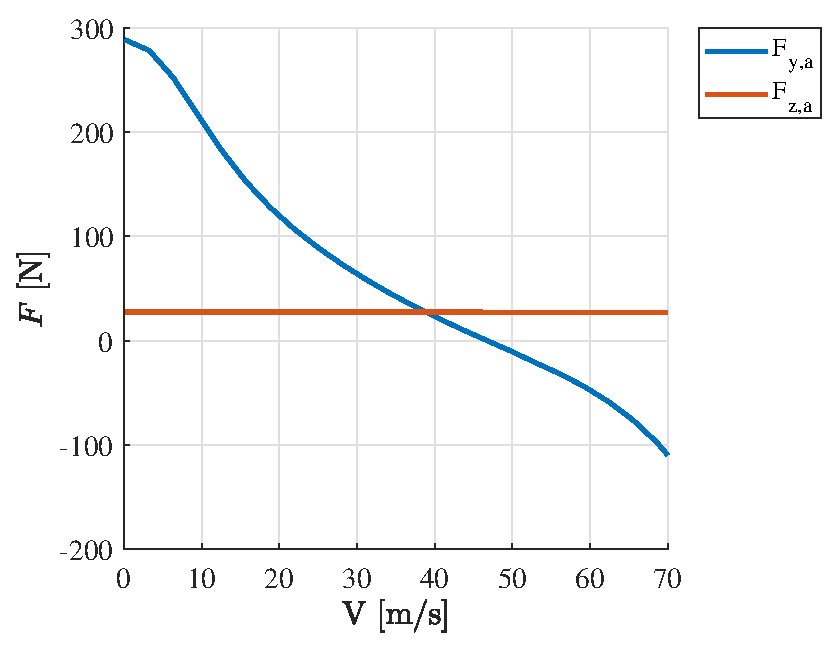
\includegraphics[width=90mm]{graficos/FAP}
%	\caption{Fuerzas sobre el rotor antipar a distintas velocidades de vuelo a nivel del mar según los ejes cuerpo y y z.}
%	\label{FAP}
%\end{figure}
%
%\begin{figure}
%	\centering
%	\subfigure[Estabilizador vertical]{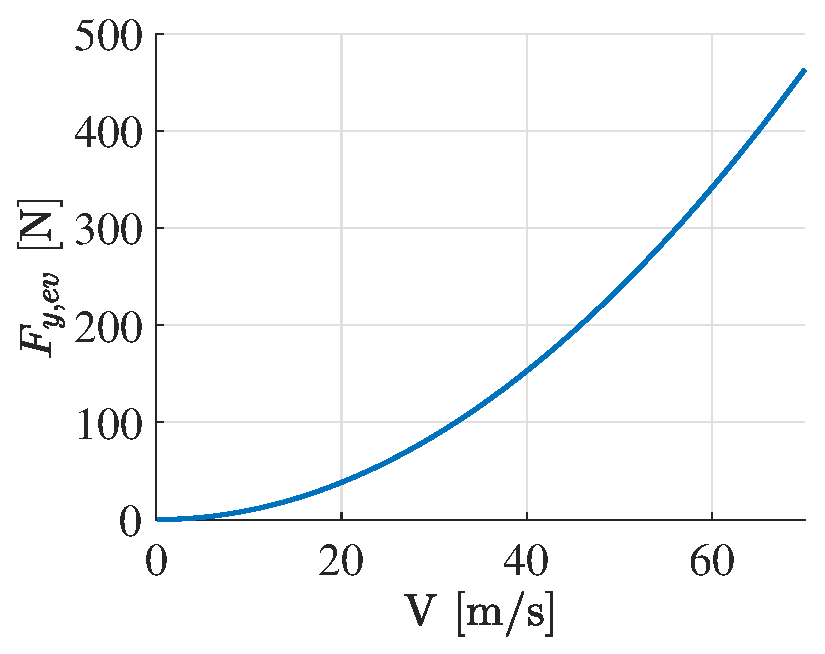
\includegraphics[width=60mm]{graficos/FEV}}
%	\subfigure[Estabilizador horizontal]{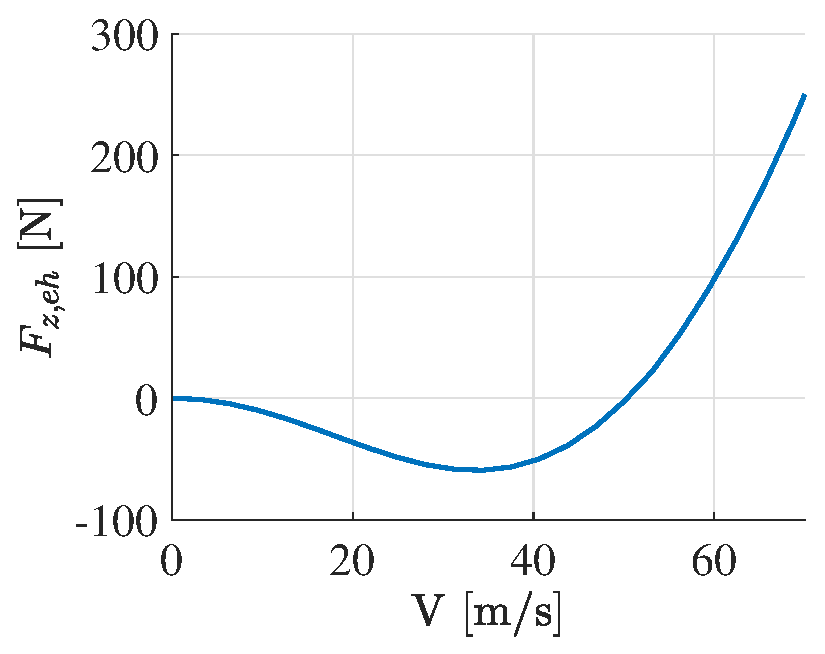
\includegraphics[width=60mm]{graficos/FEH}}
%	\caption{Fuerzas sobre los estabilizadores (a) vertical y (b) horizontal a distintas velocidades de vuelo a nivel del mar. Las fuerzas que se representan son horizontales (eje y cuerpo) para el estabilizador vertical y verticales (eje z cuerpo) para el estabilizador vertical.}
%	\label{FE}
%\end{figure}
%
%
%Se puede observar en la gráfica \ref{FAP} que las cargas sobre el rotor antipar cambian de signo, es decir, de sentido, a partir de ciertas velocidades. Esta evolución puede resultar extraña, pero el motivo se puede observar en la gráfica \ref{FAP}. Como ocurriría con un ala, el estabilizador vertical genera una carga en el eje y que aumenta con la velocidad de vuelo. Esta carga ayuda a reducir la potencia necesaria en el rotor antipar para bajas velocidades ya que ayuda a compensar el momento de giro que provoca el rotor principal. Sin embargo, estas cargas, para velocidades altas, superan a las necesarias para compensar dicho momento, y el antipar debe pasar a compensar la carga sobre el estabilizador vertical. Además, aunque su origen no es aerodinámico, el propio peso del rotor antipar supondrá una carga de valor constante que también se ha de tener en cuenta.
%
%En lo que respecta al estabilizador horizontal, a bajas velocidades genera una carga ascendente que ayuda a la estabilidad longitudinal del sistema. A altas velocidades (mayores a 50 m/s) las cargas se vuelven descendentes. Esto puede deberse a un fallo del modelo, que en situaciones límite no sea capaz de obtener buenas aproximaciones, aunque en una situación real en avance, la estela del rotor principal puede incidir sobre el estabilizador horizontal y generar cargas descendentes.
%
%Queda por tanto claro que a mayor velocidad de vuelo las cargas serán mayores, llegando hasta cargas de 300 N que la cola tendrá que soportar en vuelo a punto fijo (debidas al rotor antipar), pero mayores para vuelos a altas velocidades (400 N para vuelos a 60 m/s).
%
%\subsection{Variación de las Cargas en la Cola con el Ángulo de Ataque $\boldsymbol{\alpha_f}$}
%
%Estas simulaciones se han realizado suponiendo ángulos de ataque del fuselaje nulos, por lo que puede resultar interesante ver como evolucionan las cargas sobre los estabilizadores con el ángulo de ataque $\alpha_0$ y el ángulo de resbalamiento $\beta_f$. La gráfica \ref{FEa} representa la variación más significativa de las cargas en los estabilizadores, las cargas sobre el estabilizador horizontal. Se aprecia que su comportamiento es el de un perfil aerodinámico, incluso se aprecia un comportamiento prácticamente lineal con el ángulo de ataque. Todo esto implica que si se desean reducir las cargas en la cola, conviene volar a pequeños ángulos de ataque negativos, lo que, como se representa en la figura \ref{PMVHa}, conlleva un aumento de la potencia necesaria y por tanto del consumo a la par que una reducción de la autonomía de vuelo.
%
%\begin{figure}
%	\centering
%	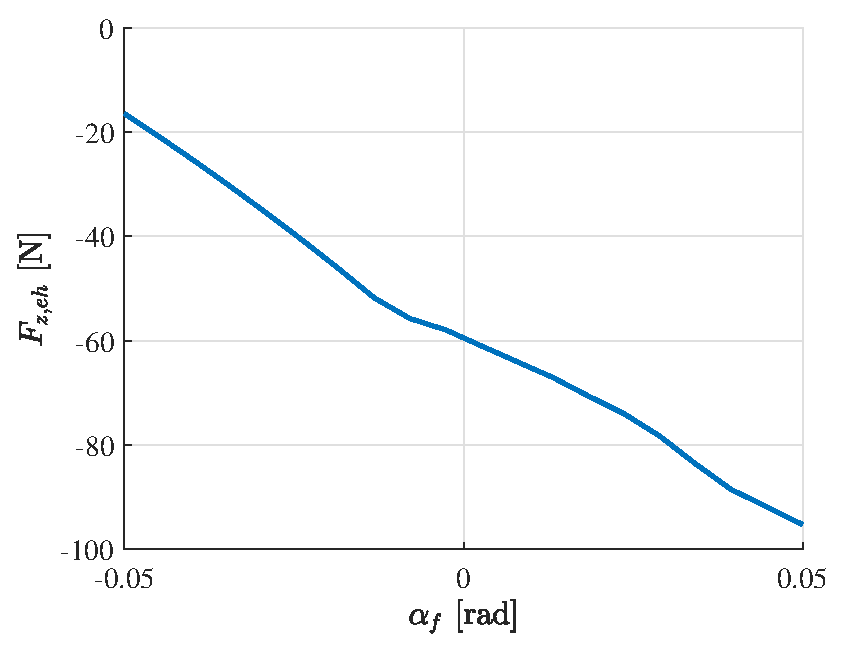
\includegraphics[width=90mm]{graficos/FEHa}
%	\caption{Fuerzas verticales (eje z cuerpo) sobre el estabilizador horizontal a distintos ángulos de ataque a nivel del mar para una velocidad de vuelo de 28 m/s.}
%	\label{FEa}
%\end{figure}
%
%\begin{figure}
%	\centering
%	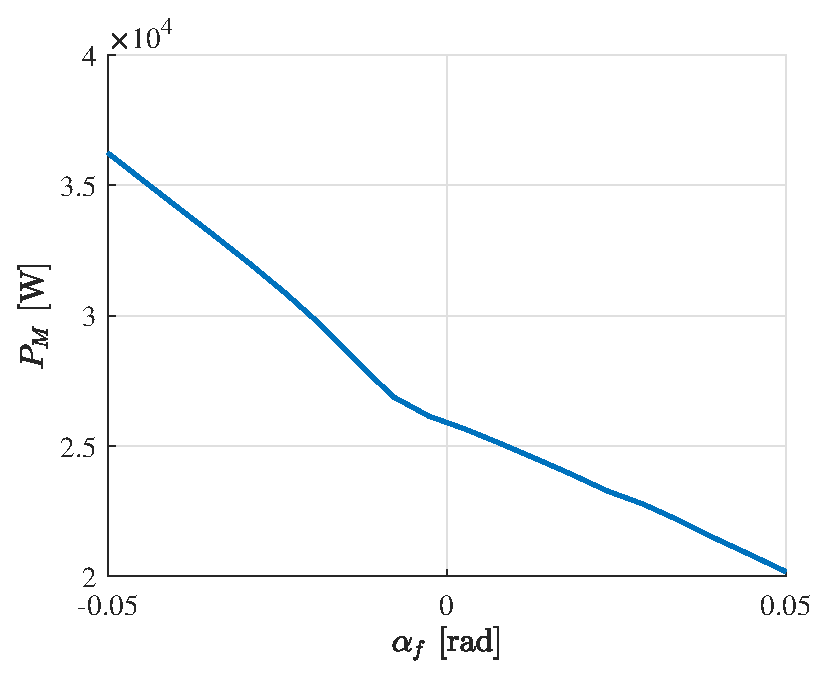
\includegraphics[width=90mm]{graficos/PMVHa}
%	\caption{Potencia necesaria para un vuelo horizontal a distintos ángulos de ataque a nivel del mar para una velocidad de vuelo de 28 m/s.}
%	\label{PMVHa}
%\end{figure}
%
%En estas circunstancias reducir el ángulo de ataque no resulta interesante, apenas variamos las cargas a costa de reducir la autonomía, pero si consideramos un vuelo con un ángulo de ataque $\alpha_f=$0.025 rad la autonomía se incrementa hasta las 5 horas y 20 minutos. Los resultados de estos cálculos se pueden encontrar en la tabla \ref{auttab2}.
%
%\begin{table}[htbp]
%	\centering
%	\begin{tabular}{|>{\columncolor{Gray}}c|c|}
%		\hline
%		\cellcolor{Gray2}Variable & \cellcolor{Gray2}Valor \\ \hline \hline
%		\cellcolor{Gray}Ángulo de ataque del fuselaje ($\alpha_f$)  & 0.025 rad \\ \hline
%		\cellcolor{Gray}Velocidad de vuelo ($V$) & 28.73 m/s \\ \hline
%		\cellcolor{Gray}Potencia necesaria ($PM$)  & 22.155 kW \\ \hline
%		\cellcolor{Gray}Consumo específico ($c_{e}$) & 9.54$\cdot$10$^-08$ kg/W$\cdot$s \\ \hline
%		\cellcolor{Gray}Autonomía ($t_{e,max}$) & 5.3231 h \\ \hline
%	\end{tabular}%
%	\caption{Parámetros relacionados con el cálculo de la autonomía del helicóptero en las condiciones de vuelo horizontal a 28.73 m/s con ángulo de ataque de 0.025 rad.}
%	\label{auttab2}
%\end{table}%
%
%\subsection{Variación de las Cargas en la Cola con el Ángulo de Resbalamiento $\boldsymbol{\beta_f}$}
%
%De manera análoga a lo hecho con el ángulo de ataque, se han calculado las variaciones de las cargas en los elementos de la cola con el ángulo de resbalamiento $\beta_f$.
%El caso del estabilizador vertical recuerda al del estabilizador horizontal del apartado anterior pero de forma inversa, la carga varía de forma casi lineal con el ángulo de resbalamiento, a mayor ángulo, menor carga (figura \ref{FEVb}). Como se ha dicho anteriormente, el estabilizador vertical ayuda a reducir la potencia necesaria para el rotor antipar, por lo que esta reducción hace necesario un nuevo cálculo de las cargas sobre el mismo. Dicho cálculo se refleja en la gráfica \ref{FAPb} y en ella se observa la tendencia esperada, las cargas aumentan con $\beta_f$, pero para comprobar si las cargas totales son menores o mayores, se ha representado en la gráfica \ref{deltafyb} que indica la variación total de las cargas horizontales debidas a estos elementos respecto a las cargas para ángulo de resbalamiento nulo.
%Esta gráfica deja claro que en lo que respecta a las cargas sobre la cola lo mas favorable es volar a ángulo de resbalamiento ligeramente positivo.  
%
%\begin{figure}
%	\centering
%	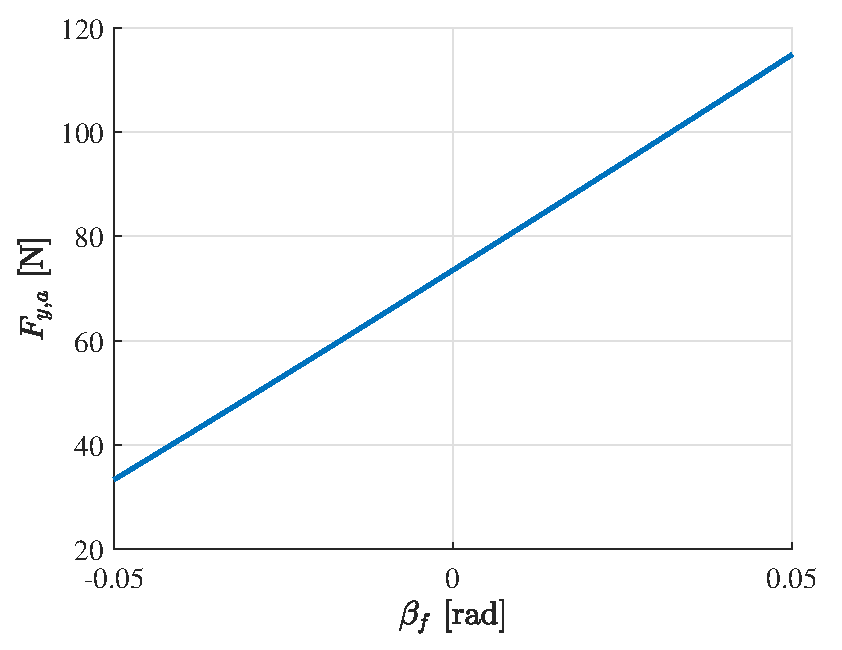
\includegraphics[width=90mm]{graficos/FAPb}
%	\caption{Fuerzas horizontales (eje y cuerpo) sobre el rotor antipar a distintos ángulos de resbalamiento a nivel del mar para un vuelo horizontal a 28 m/s.}
%	\label{FAPb}
%\end{figure}
%
%\begin{figure}
%	\centering
%	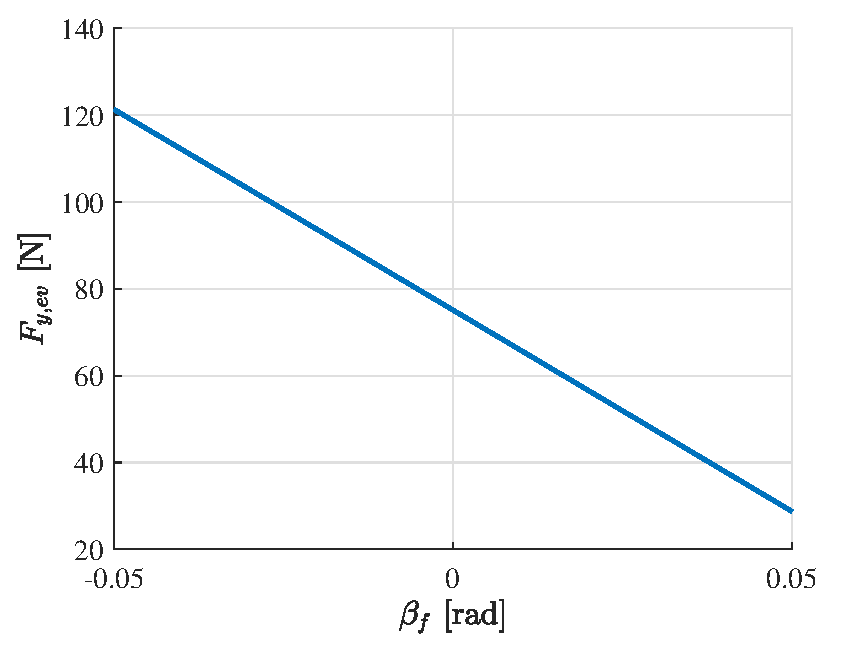
\includegraphics[width=90mm]{graficos/FEVb}
%	\caption{Fuerzas horizontales (eje y) sobre el estabilizador vertical a ángulos de resbalamiento a nivel del mar para un vuelo horizontal a 28 m/s.}
%	\label{FEVb}
%\end{figure}
%
%\begin{figure}
%	\centering
%	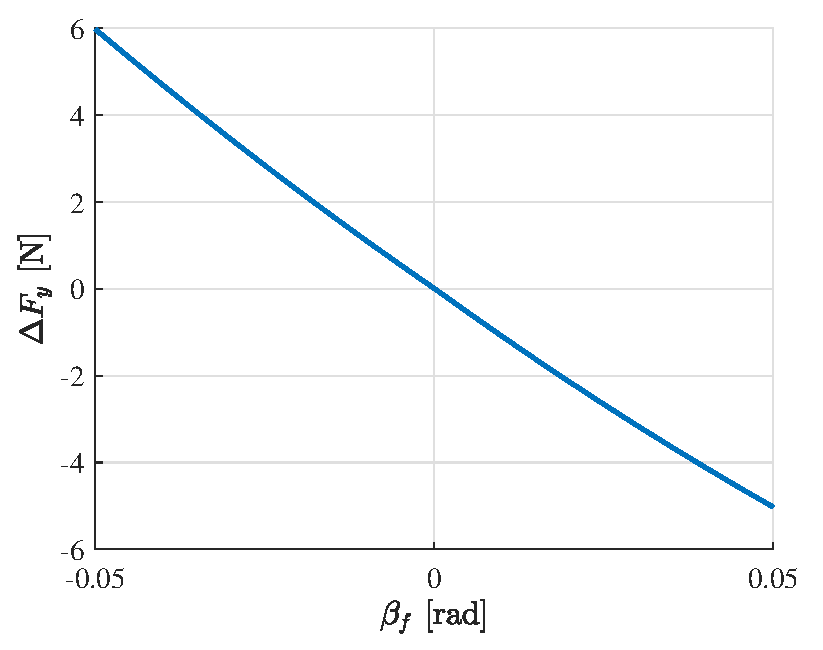
\includegraphics[width=90mm]{graficos/deltafyb}
%	\caption{Variación de la fuerza horizontal (eje y cuerpo) sobre la cola debida al estabilizador vertical y el rotor antipar a distintos ángulos de resbalamiento respecto a ángulo nulo a nivel del mar para un vuelo horizontal a 28 m/s.}
%	\label{deltafyb}
%\end{figure}
%
%\begin{figure}
%	\centering
%	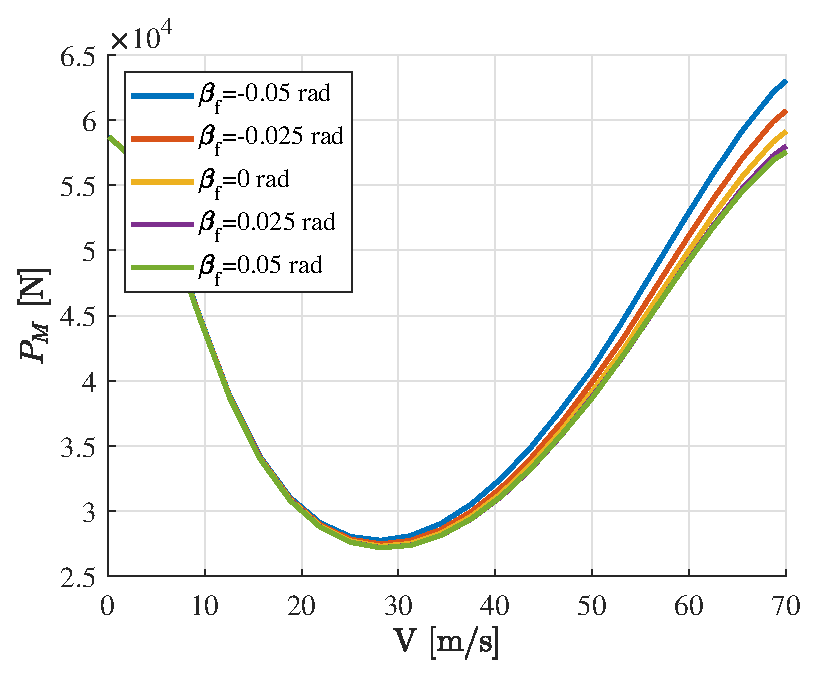
\includegraphics[width=90mm]{graficos/Potb}
%	\caption{Variación de la potencia necesaria para el vuelo horizontal a nivel del mar a distintas velocidades y ángulos de resbalamiento.}
%	\label{Potb}
%\end{figure}
%
%Para comprobar si puede resultar más eficiente volar con ángulo de resbalamiento no nulo, se ha vuelto a simular el mismo vuelo que al principio del capítulo para varios valores del ángulo de resbalamiento y los resultados de las potencias necesarias se han plasmado en la gráfica \ref{Potb} donde se observa que la potencia necesaria para el vuelo disminuye según aumenta el ángulo de resbalamiento.
%
%Todo esto indica en un primer momento que resulta mas favorable, tanto para reducir cargas como potencia necesaria, volar a pequeños ángulos de resbalamiento.
%
%Respecto al estabilizador horizontal, la gráfica \ref{FEHb} muestra que las variaciones de las cargas verticales son de 1 N como máximo, por lo que queda claro que resulta indiferente a la hora de decidir si conviene volar a un ángulo de resbalamiento u otro.
%
%
%\begin{figure}
%	\centering
%	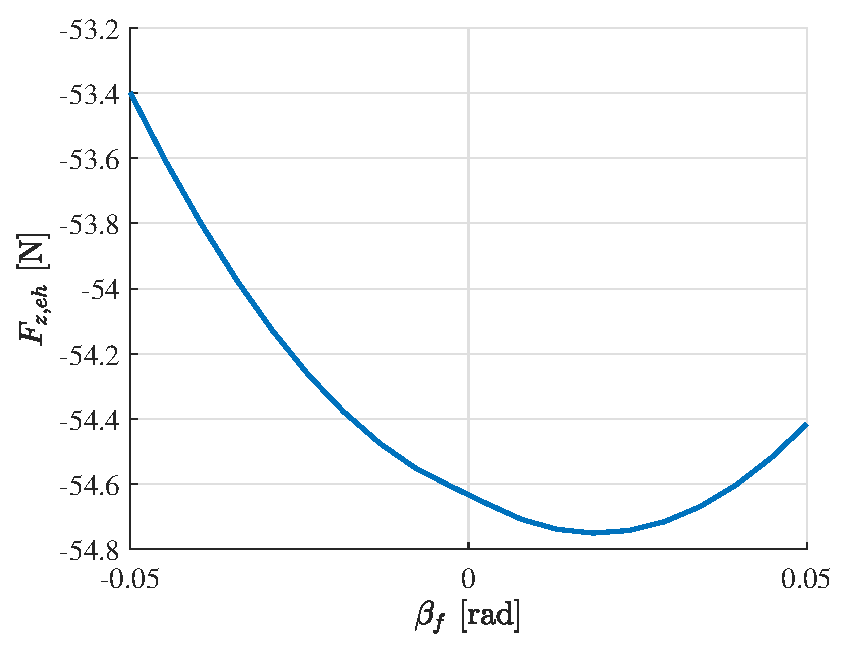
\includegraphics[width=90mm]{graficos/FEHb}
%	\caption{Fuerzas verticales (eje z cuerpo) sobre el estabilizador horizontal a ángulos de resbalamiento a nivel del mar para un vuelo horizontal a 28 m/s.}
%	\label{FEHb}
%\end{figure}

\section{Posibles Cambios en el Diseño}

Hecho un análisis de los parámetros de vuelo en distintas condiciones para el vuelo horizontal, es hora de comprobar el efecto de algunos parámetros de diseño en el vuelo. Para ello se mostrarán gráficas similares a las anteriores del mismo capítulo para diferentes valores de diferentes características de la aeronave.

\subsection{Rigidez en Batimiento $\boldsymbol{k_{\beta}}$}

Un parámetro que puede ser interesante cambiar es la rigidez de las palas en batimiento. \emph{HEROES} calcula un valor suponiendo que se quiere mantener una rigidez similar a la del rotor del helicóptero base, es decir, el Bölkow Bo 105.
Para comprobar su efecto, se ha decidido variar su valor base (denominado como $k_{\beta0}$ en las gráficas) entre el 70\% y el 130\% (tabla \ref{kbetatab}) de su valor. Los resultados de esta simulación se han reflejado en las gráficas \ref{PMVHkbeta}, \ref{EulerVHkbeta} y \ref{FRPkbeta}.

\begin{table}[htbp]
	\centering
	\begin{tabular}{|>{\columncolor{Gray}}c|c|}
		\hline
		\cellcolor{Gray} & 7231.08 \\ \cline{2-2}
		\cellcolor{Gray} & 8780.6 \\ \cline{2-2}
		\cellcolor{Gray} & 10330.12 \\ \cline{2-2}
		\cellcolor{Gray} & 11879.64 \\ \cline{2-2}
		\multirow{-5}{*}{\cellcolor{Gray}$k_\beta$ (Nm/rad)} & 13429.15 \\ \hline
	\end{tabular}%
	\caption{Valores de la rigidez en batimiento de las palas usados en la simulación, en orden ascendente de valor. El valor central es el valor que \emph{HEROES} ha otorgado al modelo de forma automática.}
	\label{kbetatab}
\end{table}%

\begin{figure}
	\centering
	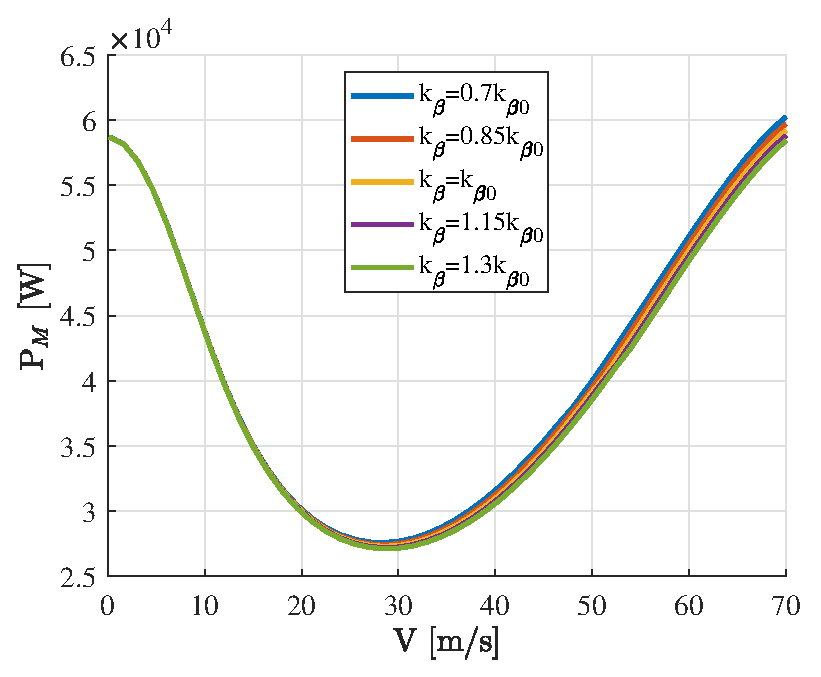
\includegraphics[width=90mm]{graficos/PMVHkbeta}
	\caption{Consumo de Potencia de la aeronave en función de la velocidad de vuelo a nivel del mar para vuelo horizontal y limitación por potencia máxima continua disponible.}
	\label{PMVHkbeta}
\end{figure}
\begin{figure}
	\centering
	\subfigure[Paso cíclico longitudinal]{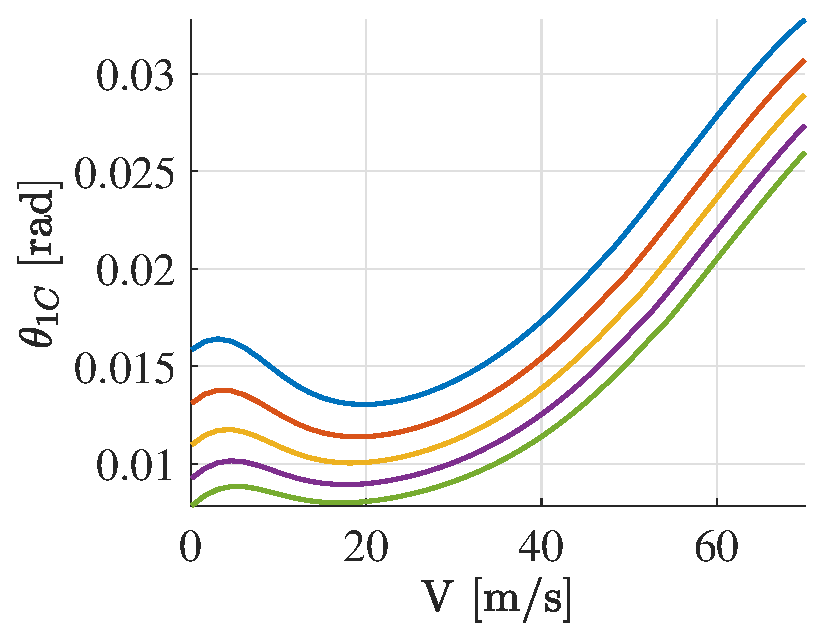
\includegraphics[width=60mm]{graficos/theta1CVHkbeta}}
	\subfigure[Paso cíclico lateral]{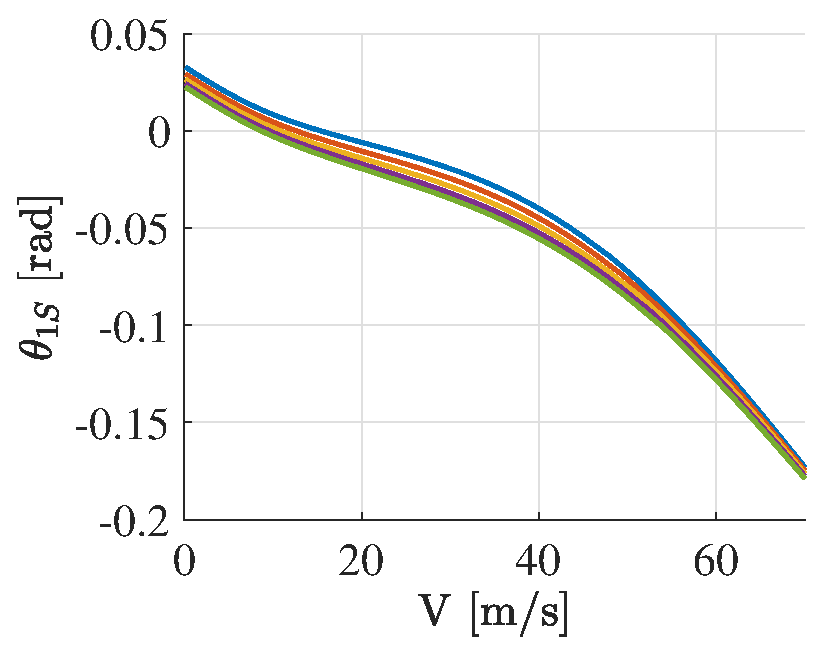
\includegraphics[width=60mm]{graficos/theta1SVHkbeta}}
	\subfigure[Paso colectivo]{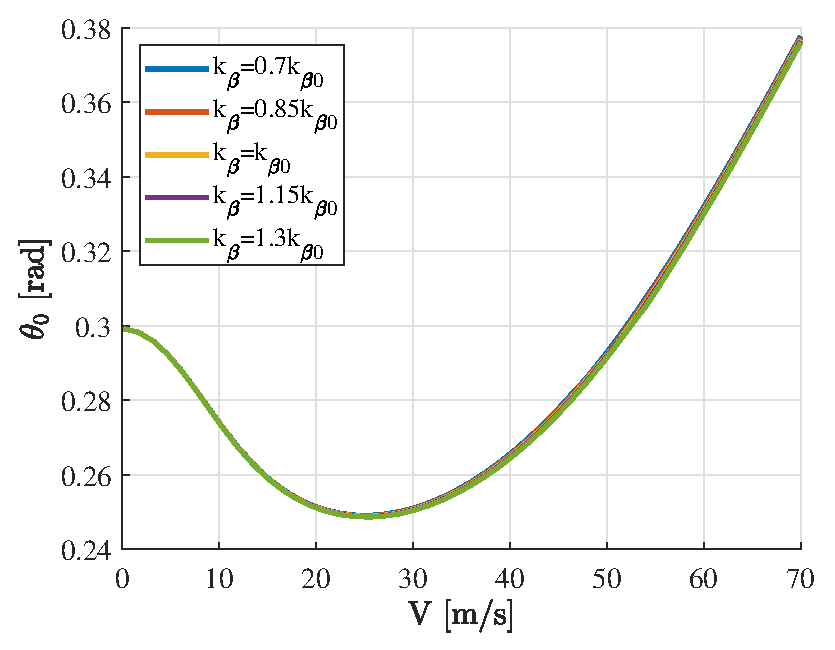
\includegraphics[width=90mm]{graficos/theta0VHkbeta}}
	\caption{Ángulos de control de la aeronave en función de la velocidad de vuelo a nivel del mar para vuelo horizontal y diferentes valores de k$_\beta$.}
	\label{ControlVHkbeta}
\end{figure}
\begin{figure}
	\centering
	\subfigure[Fuerzas longitudinales (eje x)]{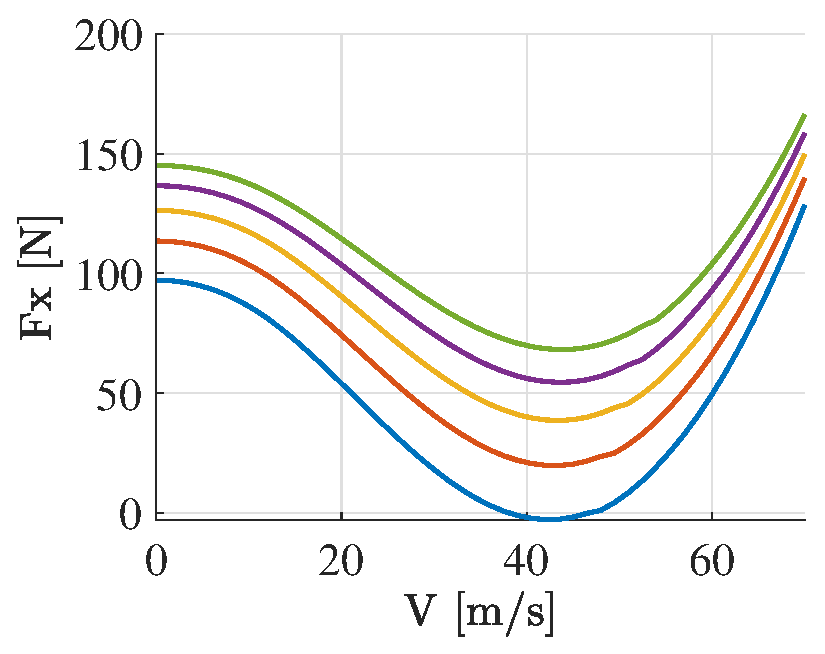
\includegraphics[width=60mm]{graficos/FRPxkbeta}}
	\subfigure[Fuerzas laterales (eje y)]{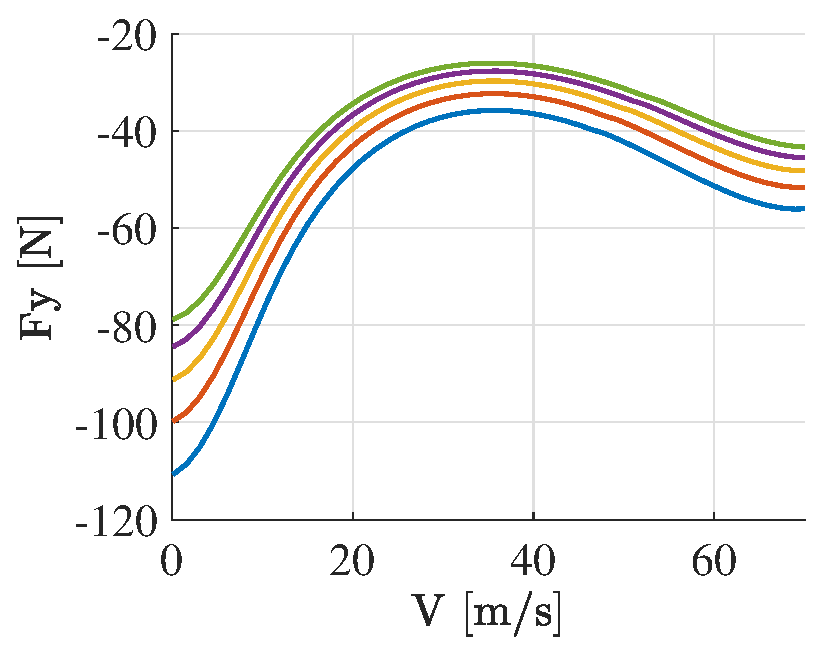
\includegraphics[width=60mm]{graficos/FRPykbeta}}
	\subfigure[Fuerzas verticales (eje z)]{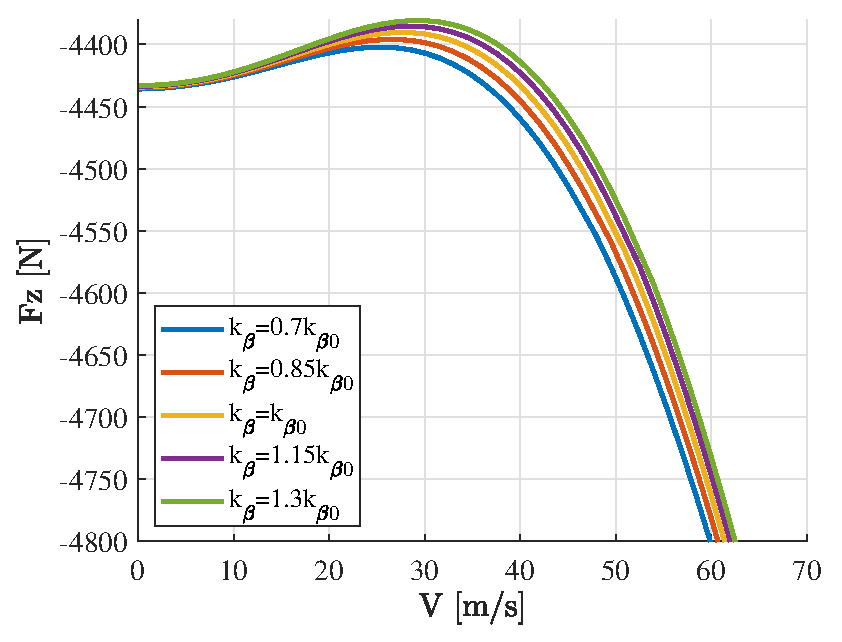
\includegraphics[width=90mm]{graficos/FRPzkbeta}}
	\caption{Fuerzas (en ejes cuerpo) sobre el rotor principal en función de la velocidad de vuelo a nivel del mar para vuelo horizontal y diferentes valores de k$_\beta$.}
	\label{FRPkbeta}
\end{figure}

Lo primero que se observa es que los cambios no son excesivamente llamativos, pero existen. En el caso de la potencia necesaria para el vuelo se observa en \ref{PMVHkbeta} que a bajas velocidades de vuelo los resultados no dependen de $k_\beta$, pero según aumenta la velocidad también lo hacen las diferencias en los resultados. Independientemente del valor de la velocidad, los resultados para una rigidez de batimiento mayor son mas favorables, es decir, la potencia necesaria para el vuelo es menor. Sin embargo, este resultado no tiene en cuenta que como consecuencia de llevar a cabo este cambio en un modelo real, las cargas sobre las palas aumentan y por tanto se han de realizar cambios también en el rotor y las palas, lo cual puede suponer aumentos de masa y de coste. En la gráfica \ref{kbetapala} se han representado el caso de máxima rigidez en batimiento anterior junto a un caso con un aumento de masa de pala de un 20\% (tabla \ref{bmtab}), lo que equivaldría a cambiar el material de fabricación de las palas para dotarlas de mayor rigidez (sin tener en cuenta posibles cambios de masa en el propio rotor). De estos resultados se observa que el aumento de masa contrarresta el efecto del aumento de rigidez, por lo que será necesario un análisis mas exhaustivo de los materiales disponibles, costes y necesidades de la aeronave para poder tomar una decisión acerca de aumentar la rigidez del rotor.

\begin{table}[htbp]
	\centering
	\begin{tabular}{|>{\columncolor{Gray}}c|c|}
		\hline
		\cellcolor{Gray}Masa de pala original & 18.798 kg \\ \hline
		\cellcolor{Gray}Masa de pala 20\% mayor & 22.558 kg \\ \hline
	\end{tabular}%
	\caption{Valores de las masas de las palas original y aumentado un 20\% suponiendo un cambio de material en su fabricación.}
	\label{bmtab}
\end{table}%

\begin{figure}
	\centering
	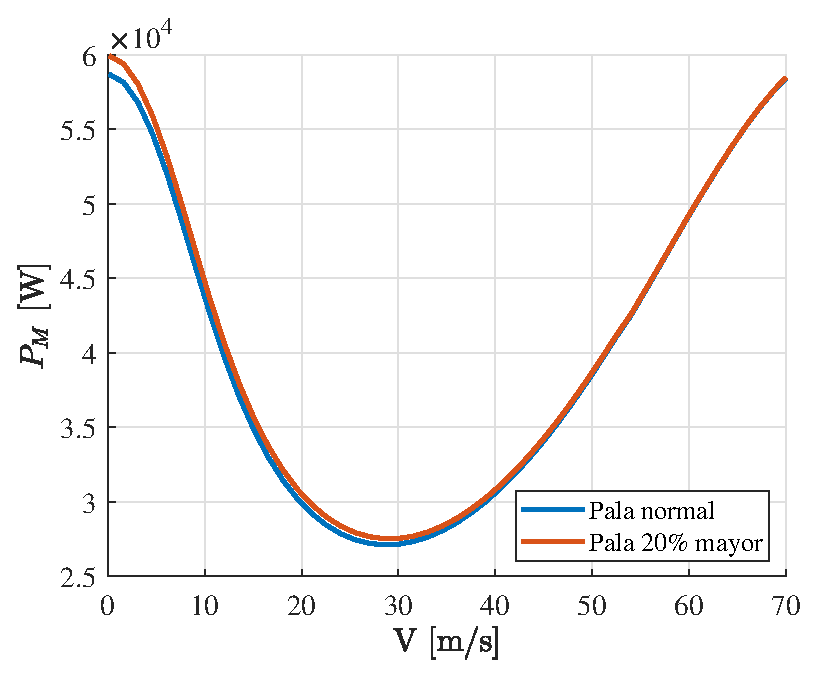
\includegraphics[width=90mm]{graficos/PMbm20}
	\caption{Potencia necesaria para un vuelo horizontal a nivel del mar a distintas velocidades de vuelo para un helicóptero de rigidez en batimiento $k_\beta$=13429.15 Nm/rad y masas de pala original y un 20\% mayor.}
	\label{kbetapala}
\end{figure}

En cuanto al resto de resultados, se puede observar en \ref{ControlVHkbeta} que el paso colectivo se mantiene prácticamente constante con $k_\beta$, por lo que los únicos cambios que se observan son en los ángulos de paso cíclico lateral y longitudinal. En ambos casos el aumento de la rigidez lleva acompañado una disminución de los ángulos de paso cíclico que en el caso del longitudinal se observa que la diferencia entre los valores máximo y mínimo de $k_\beta$ de la simulación supone alrededor de 0.005 rad, mientras que en el lateral las diferencias alcanzan valores de entre 0.01 y 0.012 rad. Estos cambios de menos de un grado son asumibles por lo que no supondría ningún problema a la hora de variar la rigidez en batimiento del rotor principal.

Donde se observan cambios mayores es en las cargas que aparecen en el rotor principal (gráfica \ref{FRPkbeta}). Lo primero que se observa es que las cargas verticales y laterales no solo no aumentan, sino que disminuyen. Las cargas verticales sufren una variación pequeña, que aumenta con la velocidad, pero esta variación llega a valores de unos 50 N a velocidades de alrededor de 40 m/s, lo que comparado con los valores de alrededor de 4475 N a los que están sometidos lo diferentes modelos a esas velocidades resulta despreciable.

En el caso de las fuerzas laterales las variaciones máximas se dan para bajas velocidades de vuelo, llegando a valores de 30 N, que a 40 m/s se ven reducidas a apenas 10 N de diferencia. Pese a que estas variaciones sean menores a las que aparecen las fuerzas verticales, su valor relativo es mucho mayor ya que los valores de las cargas son de alrededor de 100 N a velocidades muy bajas y de 35 N a 40 m/s. Esto supone una disminución importante de las cargas, al menos en el eje lateral.

Sin embargo, las cargas más críticas serían las que aparecen en el eje longitudinal del helicóptero, cuyas variaciones máximas entre las distintas configuraciones son de hasta 60 N, llegando a cargas máximas un 25\% mayores que las esperadas en el modelo original. Además el modelo más rígido sufre cargas del orden de 70 N para velocidades de vuelo en las que el modelo menos rígido no sufre ninguna carga. Estos cambios por tanto harían necesario un análisis de la estructura del rotor para comprobar si pudiese soportar las nuevas cargas o si por el contrario, conviene reducir la rigidez y con ello las cargas para reducir costes o peso.

\subsection{Integración de las Diferentes Cargas de Pago}

En el capítulo anterior se modelizaron 3 cargas de pago diferentes y se mostraron los cálculos para integrarlas en el fuselaje del helicóptero suponiendo que en todo momento se encuentran en su interior y por lo tanto no es necesario un cálculo aerodinámico. Estudiar como varían los parámetros de vuelo con la carga y su posición es importante a fin de poder realizar la integración ideal en cada caso.
Para poder comprobar como afecta la carga al vuelo, se realizarán las mismas suposiciones en las condiciones de vuelo que al principio del capítulo, sumando a ellas que en todas las configuraciones el MTOW será de 450 kg, es decir, habrá que calcular en cada carga un modelo del helicóptero cuya masa sea de 450 kg menos la masa de la propia carga de pago, para luego incorporar la carga de pago como ya se ha mostrado. De no seguir este proceso, estaríamos volando por encima del MTOW requerido en todo momento.

\begin{figure}
	\centering
	\subfigure[Potencia necesaria para el vuelo para difeerentes cargas de pago situadas en la proyección del centro de masas de la aeronave en vacío sobre el suelo.]{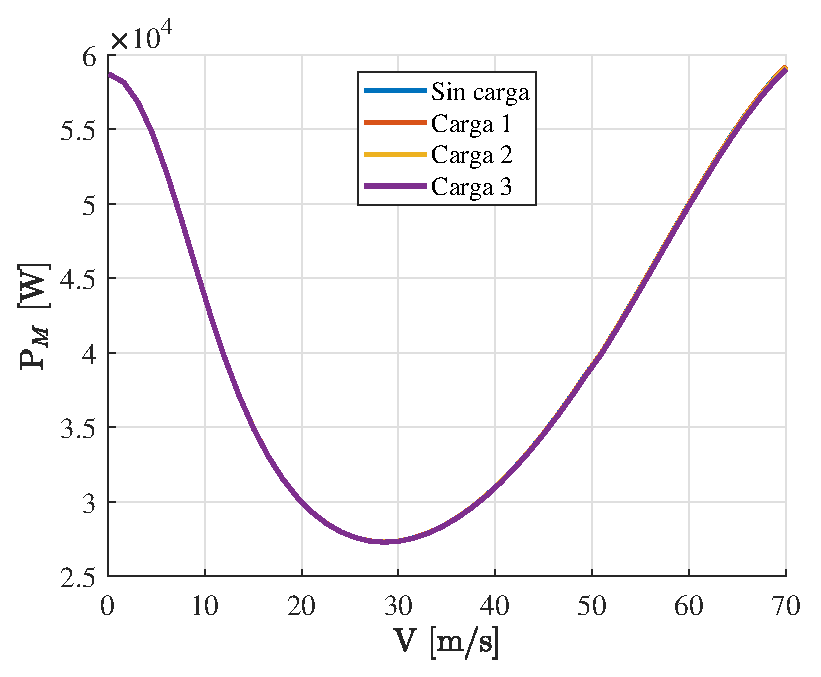
\includegraphics[width=60mm]{graficos/PMVHMPLcdg}}
	\subfigure[Potencia necesaria para el vuelo para difeerentes cargas de pago  situadas en $l_x$=1.3 m y $l_y$=-0.2 m.]{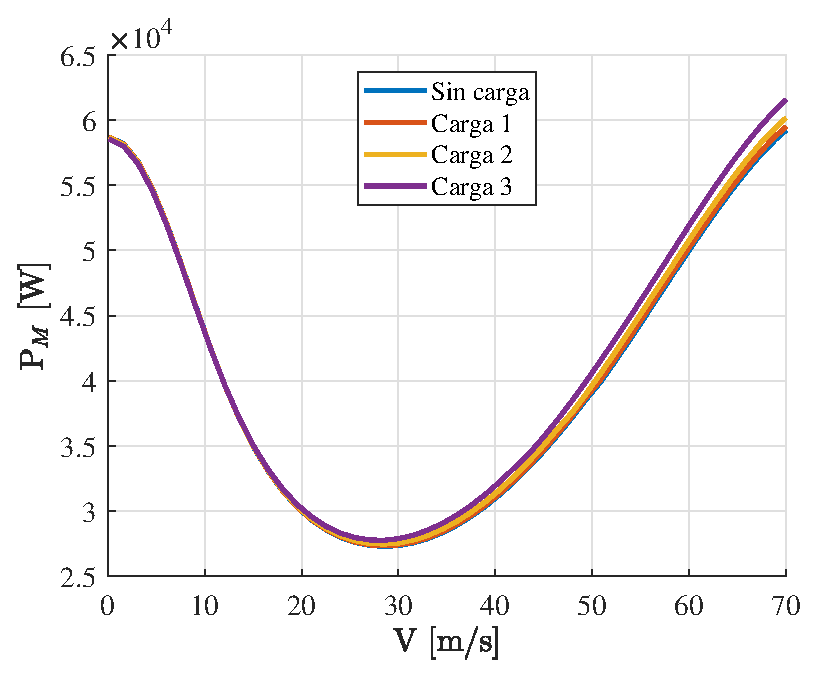
\includegraphics[width=60mm]{graficos/PMVHMPLnocdg}}
	\caption{Consumo de Potencia de la aeronave en función de la velocidad de vuelo a nivel del mar para vuelo horizontal para diferentes cargas de pago en posiciones distintas.}
	\label{PMVHMPL}
\end{figure}
\begin{figure}
	\centering
	\subfigure[Ángulo de paso colectivo del rotor principal durante el vuelo para difeerentes cargas de pago situadas en la proyección del centro de masas de la aeronave en vacío sobre el suelo.]{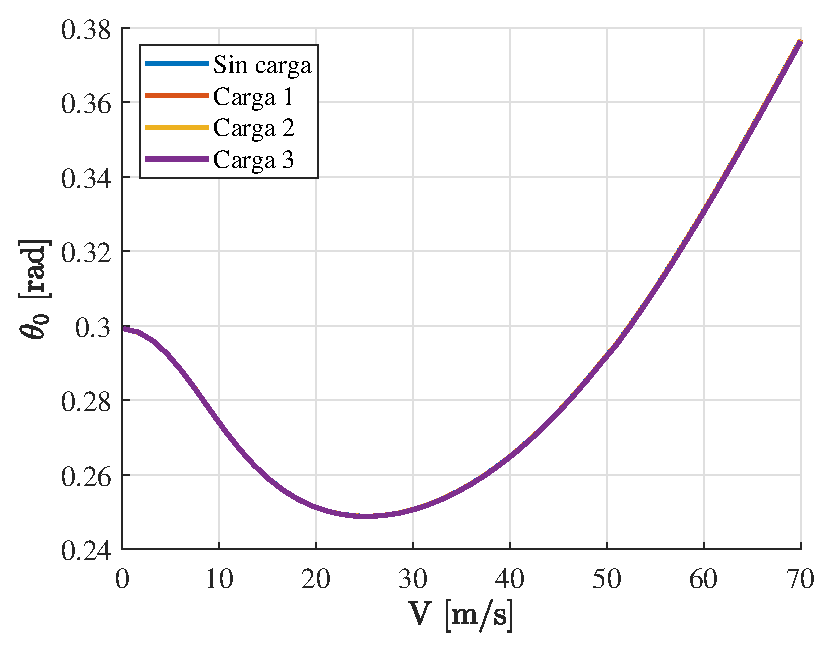
\includegraphics[width=60mm]{graficos/theta0VHMPLcdg}}
	\subfigure[Ángulo de paso colectivo del rotor principal durante el vuelo para difeerentes cargas de pago situadas en $l_x$=1.3 m y $l_y$=-0.2 m.]{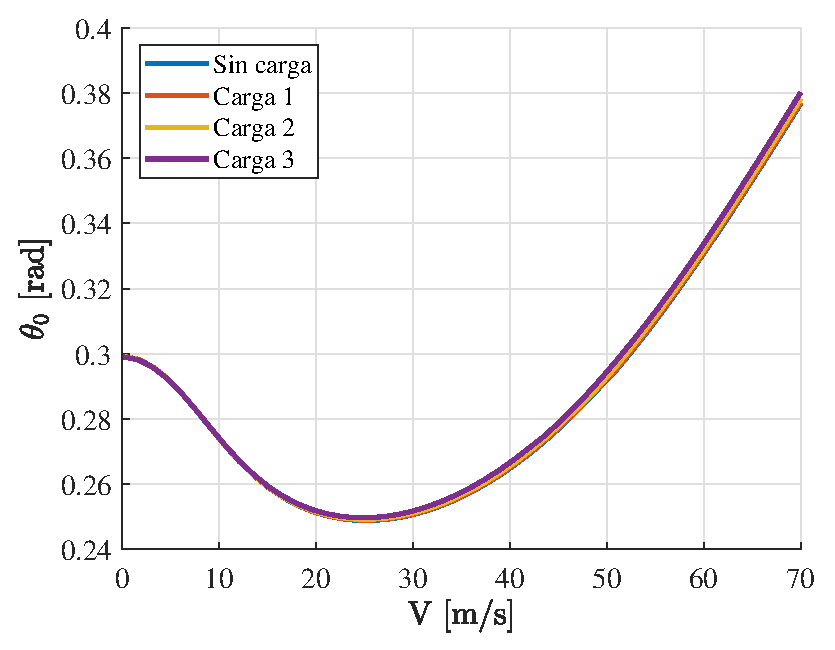
\includegraphics[width=60mm]{graficos/theta0VHMPLnocdg}}
	\caption{Ángulos de paso colectivo del rotor principal de la aeronave en función de la velocidad de vuelo a nivel del mar para vuelo horizontal para diferentes cargas de pago en posiciones distintas.}
	\label{Theta0VHMPL}
\end{figure}
\begin{figure}
	\centering
	\subfigure[Ángulo de paso cíclico longitudinal del rotor principal durante el vuelo para difeerentes cargas de pago situadas en la proyección del centro de masas de la aeronave en vacío sobre el suelo.]{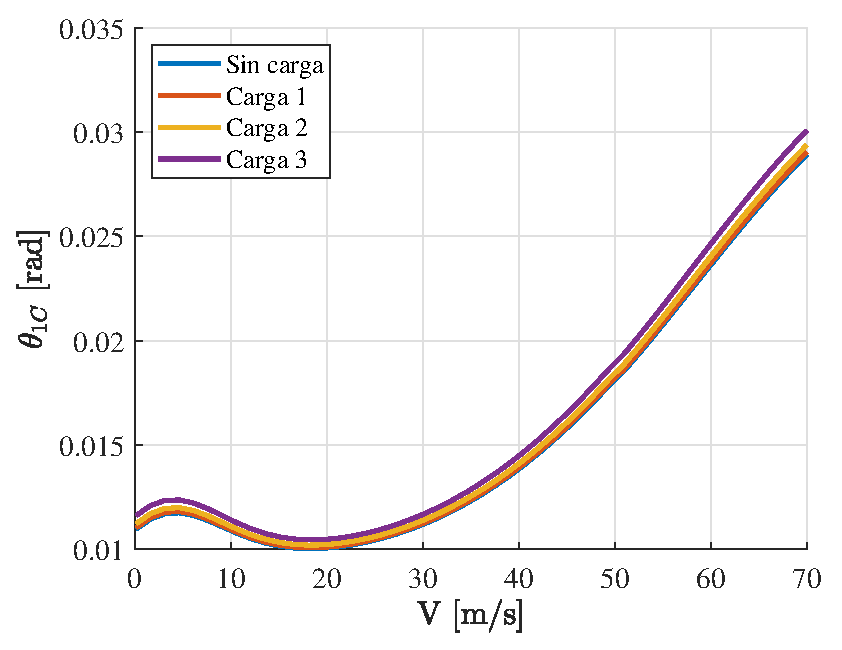
\includegraphics[width=60mm]{graficos/theta1CVHMPLcdg}}
	\subfigure[Ángulo de paso cíclico longitudinal del rotor principal durante el vuelo para difeerentes cargas de pago situadas en $l_x$=1.3 m y $l_y$=-0.2 m.]{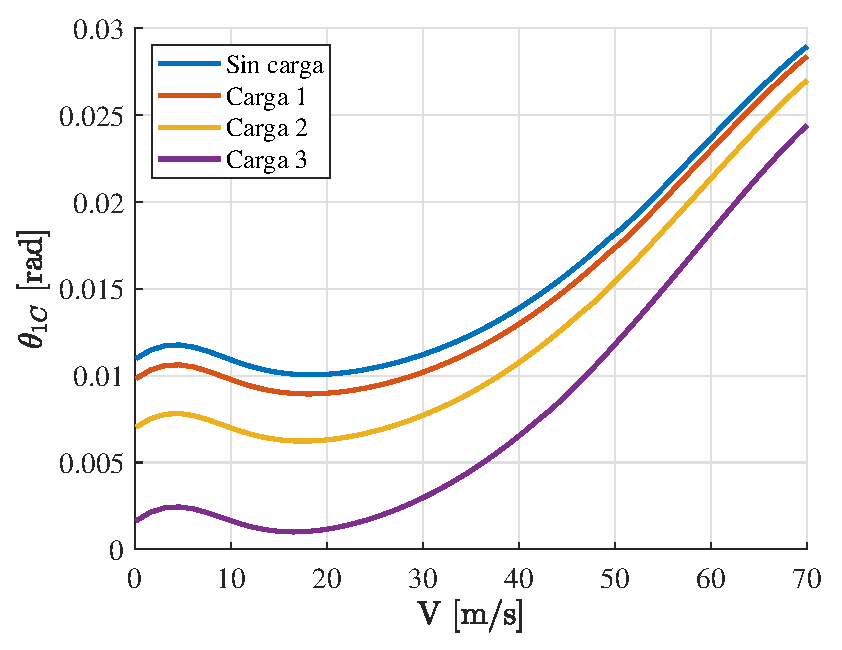
\includegraphics[width=60mm]{graficos/theta1CVHMPLnocdg}}
	\caption{Ángulos de paso cíclico longitudinal del rotor principal de la aeronave en función de la velocidad de vuelo a nivel del mar para vuelo horizontal para diferentes cargas de pago en posiciones distintas.}
	\label{Theta1CVHMPL}
\end{figure}
\begin{figure}
	\centering
	\subfigure[Ángulo de paso cíclico lateral del rotor principal durante el vuelo para difeerentes cargas de pago situadas en la proyección del centro de masas de la aeronave en vacío sobre el suelo.]{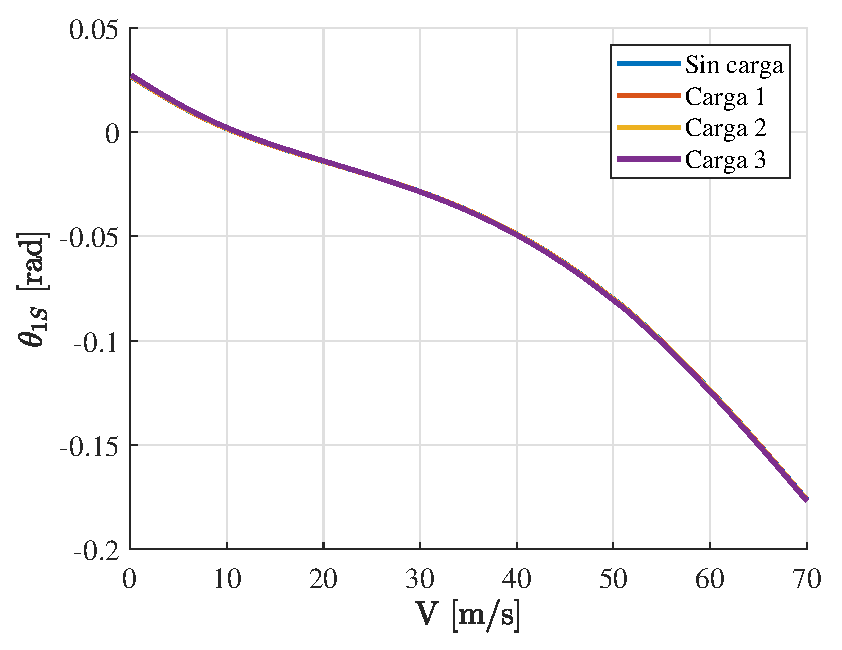
\includegraphics[width=60mm]{graficos/theta1SVHMPLcdg}}
	\subfigure[Ángulo de paso cíclico lateral del rotor principal durante el vuelo para difeerentes cargas de pago situadas en $l_x$=1.3 m y $l_y$=-0.2 m.]{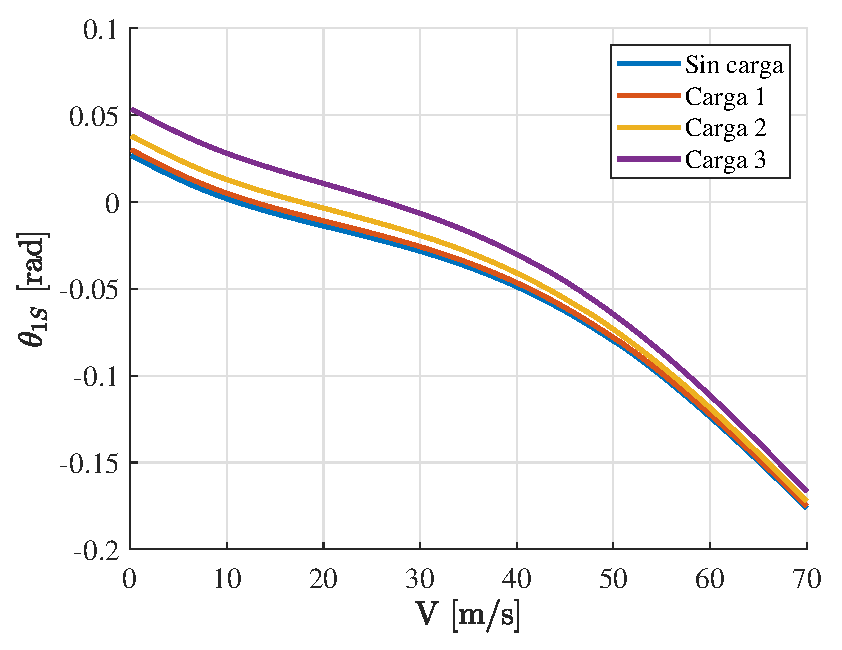
\includegraphics[width=60mm]{graficos/theta1SVHMPLnocdg}}
	\caption{Ángulos de paso cíclico lateral del rotor principal de la aeronave en función de la velocidad de vuelo a nivel del mar para vuelo horizontal para diferentes cargas de pago en posiciones distintas.}
	\label{Theta1SVHMPL}
\end{figure}
\begin{figure}
	\centering
	\subfigure[Ángulo de cabeceo de la aeronave durante el vuelo para difeerentes cargas de pago situadas en la proyección del centro de masas de la aeronave en vacío sobre el suelo.]{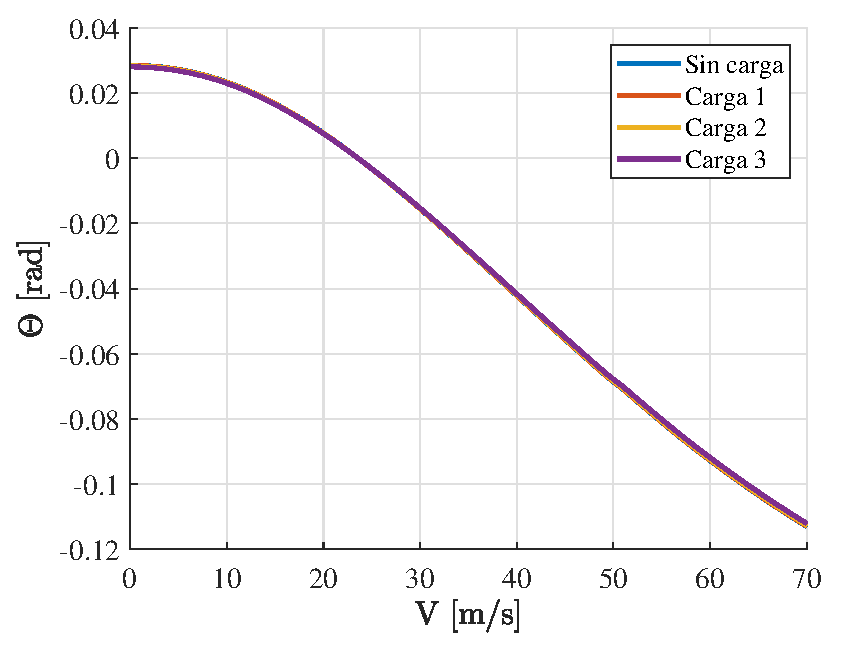
\includegraphics[width=60mm]{graficos/CabVHMPLcdg}}
	\subfigure[Ángulo de cabeceo de la aeronave durante el vuelo para difeerentes cargas de pago situadas en $l_x$=1.3 m y $l_y$=-0.2 m.]{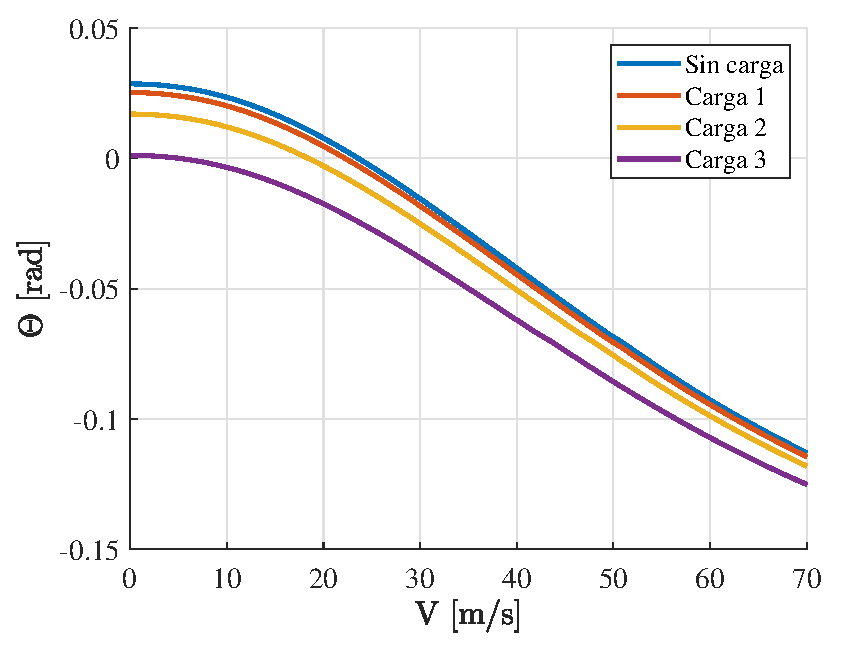
\includegraphics[width=60mm]{graficos/CabVHMPLnocdg}}
	\caption{Ángulos de cabeceo de la aeronave en función de la velocidad de vuelo a nivel del mar para vuelo horizontal para diferentes cargas de pago en posiciones distintas.}
	\label{ThetaVHMPL}
\end{figure}
\begin{figure}
	\centering
	\subfigure[Ángulo de balanceo de la aeronave durante el vuelo para difeerentes cargas de pago situadas en la proyección del centro de masas de la aeronave en vacío sobre el suelo.]{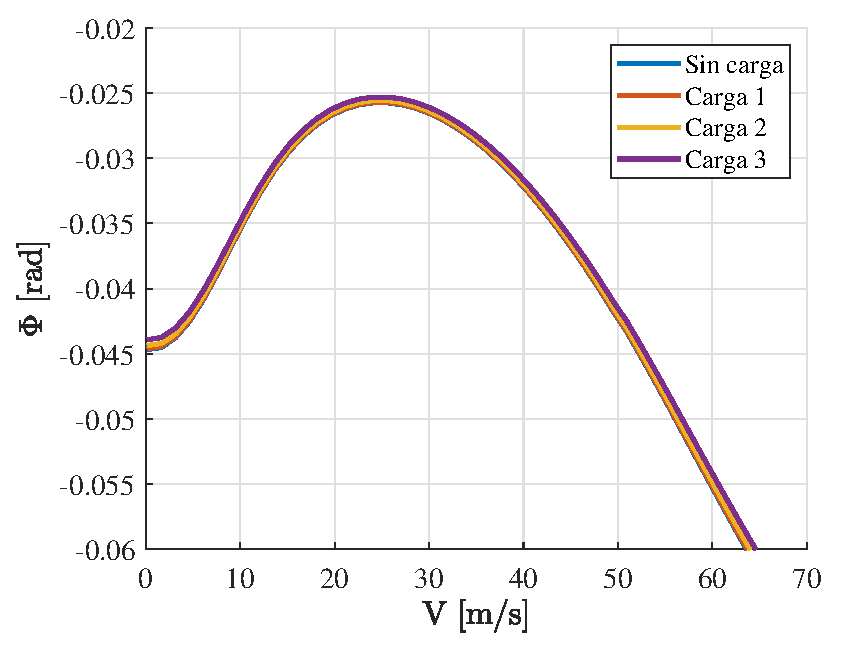
\includegraphics[width=60mm]{graficos/BalanVHMPLcdg}}
	\subfigure[Ángulo de balanceo de la aeronave durante el vuelo para difeerentes cargas de pago situadas en $l_x$=1.3 m y $l_y$=-0.2 m.]{\includegraphics[width=60mm]{graficos/BalanVHMPLnocdg}}
	\caption{Ángulos de balanceo de la aeronave en función de la velocidad de vuelo a nivel del mar para vuelo horizontal para diferentes cargas de pago en posiciones distintas.}
	\label{PhiVHMPL}
\end{figure}
\begin{figure}
	\centering
	\subfigure[Ángulo de paso colectivo del rotor antipar durante el vuelo para difeerentes cargas de pago situadas en la proyección del centro de masas de la aeronave en vacío sobre el suelo.]{\includegraphics[width=60mm]{graficos/theta0VHraMPLcdg}}
	\subfigure[Ángulo de paso colectivo del rotor antipar durante el vuelo para difeerentes cargas de pago situadas en $l_x$=1.3 m y $l_y$=-0.2 m.]{\includegraphics[width=60mm]{graficos/theta0VHraMPLnocdg}}
	\caption{Ángulos de paso colectivo del rotor antipar de la aeronave en función de la velocidad de vuelo a nivel del mar para vuelo horizontal para diferentes cargas de pago en posiciones distintas.}
	\label{Theta0VHraMPL}
\end{figure}

Las simulaciones se han realizado para las configuraciones sin carga y para cada una de las cargas en dos posiciones, sobre la proyección del centro de masas del helicóptero sin la carga sobre el suelo y para una posición de la carga en en suelo tal que $l_x$=1.3 m y $l_y$=-0.2 m, es decir, con las cámaras situadas en la parte delantera del helicóptero y desviadas ligeramente hacia un lateral del fuselaje. Los resultados de estas simulaciones se han reflejado en las gráficas \ref{PMVHMPL}, \ref{Theta0VHMPL}, \ref{Theta1CVHraMPL}, \ref{Theta1SVHMPL}, \ref{ThetaVHMPL}, \ref{PhiVHMPL} y \ref{Theta0VHraMPL}.

De los resultados se puede apreciar que en caso de colocar la carga de pago sobre la proyección las condiciones de vuelo apenas varían, por lo que los cálculos realizados para la configuración sin carga en vuelo horizontal se pueden asumir que sirven para cualquier carga siempre y cuando esté situada en ese punto.

Los resultados mas interesantes se dan cuando la carga se desplaza de dicho punto, siendo los casos más desfavorables los de mayor masa de carga de pago. En la gráfica \ref{PMVHMPL} se observa que a bajas velocidades de vuelo las diferencias son inapreciables, pero al aumentar la misma, lo hacen también las diferencias. Aún así, las diferencias en las potencias necesarias no son excesivas, llegando a valores de cerca de 2000 W para velocidades de 60 m/s.

En lo que respecta al ángulo de paso colectivo del rotor principal, al ser una configuración muy similar a la original y tener que sustentar el mismo peso, apenas varía con la carga ni la velocidad como se puede apreciar en la gráfica \ref{Theta0VHMPL}. Diferente es el caso de los ángulos de paso cíclico, tanto longitudinal como lateral. En el caso del ángulo de paso cíclico longitudinal, se ve en la gráfica \ref{Theta1CVHMPL} que a mayor carga, menor es su valor. Esto se explica fácilmente al observar la posición de la carga; una carga en la zona frontal del helicóptero adelantará el centro de masas del mismo, lo que contribuye a disminuir el ángulo de cabeceo (gráfica \ref{ThetaVHMPL}) y, por tanto, la necesidad de un ángulo de paso cíclico longitudinal que permita el vuelo en avance. Si el fuselaje tiene un ángulo de cabeceo tal que la perpendicular al plano del rotor tenga la dirección de avance, no es necesario un paso cíclico que redirija la fuerza en esa dirección.

Con el ángulo de paso cíclico lateral pasa algo similar, el desequilibrio másico que supone colocar una carga en una posición desplazada lateralmente del centro de masas del helicóptero provoca una variación en el ángulo de balanceo del vehículo (gráfica \ref{PMVHMPL}) que en este caso contribuye al desequilibrio ya existente, por lo que el paso cíclico lateral necesario para poder mantener la aeronave en equilibrio aumenta, al contrario de lo que pasaba con el paso longitudinal.

Por último se ha representado en la gráfica \ref{Theta0VHraMPL} la variación del ángulo de paso colectivo del rotor antipar necesario para equilibrar cada uno de los casos descritos, pero al igual que pasaba con el del rotor principal, no sufre cambios excesivos.

\subsection*{Variación de los Parámetros de Vuelo con la Posición de la Carga de Pago}

Visto el efecto de la propia carga sobre los parámetros de vuelo, conviene comprobar el efecto de la posición de una misma carga volando a una velocidad determinada, por lo que en este apartado se reflejarán y comentarán los resultados de simular vuelos horizontales a velocidad constante para las cargas 2 y 3 en función de la posición de la misma dentro de los márgenes establecidos en el capítulo anterior.

Como comentario general, se puede observar que el cambio de la carga apenas influye en los efectos de su posición, variando ligeramente eso si las diferentes características a analizar.

\begin{figure}
	\centering
	\subfigure[Potencia necesaria para el vuelo en función de la posición relativa a $O_f$ de la carga 2 para una velocidad de vuelo de 10 m/s.]{\includegraphics[width=60mm]{graficos/PMVH2lxy10ms}}
	\subfigure[Potencia necesaria para el vuelo en función de la posición relativa a $O_f$ de la carga 2 para una velocidad de vuelo de 50 m/s.]{\includegraphics[width=60mm]{graficos/PMVH2lxy50ms}}
	\caption{Consumo de Potencia de la aeronave en función de la posición relativa a $O_f$ de la carga 2.}
	\label{PMVH2lxy}
\end{figure}
\begin{figure}
	\centering
	\subfigure[Potencia necesaria para el vuelo en función de la posición relativa a $O_f$ de la carga 3 para una velocidad de vuelo de 10 m/s.]{\includegraphics[width=60mm]{graficos/PMVH3lxy10ms}}
	\subfigure[Potencia necesaria para el vuelo en función de la posición relativa a $O_f$ de la carga 3 para una velocidad de vuelo de 50 m/s.]{\includegraphics[width=60mm]{graficos/PMVH3lxy50ms}}
	\caption{Consumo de Potencia de la aeronave en función de la posición relativa a $O_f$ de la carga 3.}
	\label{PMVH3lxy}
\end{figure}

Comenzando por la potencia, los resultado resultan bastante curiosos; las gráficas \ref{PMVH2lxy} y \ref{PMVH3lxy} muestran que a bajas velocidades la potencia necesaria para el vuelo aumenta según disminuye $l_y$, es decir, es mayor cuanto mas a la izquierda del fuselaje esté situada la carga y también aumenta para cargas alejadas longitudinalmente del centro de gravedad de la aeronave sin carga ($x_{CG}=0.0972$). Sin embargo, a altas velocidades este comportamiento se invierte para el eje longitudinal, siendo los puntos de menor consumo aquellos en los que la carga está situada sobre el centro de gravedad de la aeronave. En el eje lateral, vuelve a repetirse el mismo comportamiento, la potencia necesaria disminuye para cargas situadas hacia la derecha del fuselaje, pero en esta ocasión aparece un mínimo alrededor de $l_y=0.2$, por lo que desplazar aún más la carga resulta perjudicial en términos de potencia. Además, a estas velocidades, estos cambios pueden suponer una reducción de hasta 10 kW respecto a valores extremos de posición, a diferencia de a bajas velocidades donde las diferencias apenas alcanzan el valor de 1 kW.

Comparando los efectos de ambas cargas, se observa que a bajas velocidades su comportamiento es prácticamente idéntico, pero a altas velocidades las cargas más pesadas y de mayor tamaño requieren de un consumo ligeramente mayor de potencia en posiciones distintas de la óptima.

\begin{figure}
	\centering
	\subfigure[Ángulo de paso colectivo del rotor principal en función de la posición relativa a $O_f$ de la carga 2 para una velocidad de vuelo de 10 m/s.]{\includegraphics[width=60mm]{graficos/theta0VH2lxy10ms}}
	\subfigure[Ángulo de paso colectivo del rotor principal en función de la posición relativa a $O_f$ de la carga 2 para una velocidad de vuelo de 50 m/s.]{\includegraphics[width=60mm]{graficos/theta0VH2lxy50ms}}
	\caption{Ángulo de paso colectivo del rotor principal en función de la posición relativa a $O_f$ de la carga 2.}
	\label{theta0VH2lxy}
\end{figure}
\begin{figure}
	\centering
	\subfigure[Ángulo de paso colectivo del rotor principal en función de la posición relativa a $O_f$ de la carga 3 para una velocidad de vuelo de 10 m/s.]{\includegraphics[width=60mm]{graficos/theta0VH3lxy10ms}}
	\subfigure[Ángulo de paso colectivo del rotor principal en función de la posición relativa a $O_f$ de la carga 3 para una velocidad de vuelo de 50 m/s.]{\includegraphics[width=60mm]{graficos/theta0VH3lxy50ms}}
	\caption{Ángulo de paso colectivo del rotor principal en función de la posición relativa a $O_f$ de la carga 3.}
	\label{theta0VH3lxy}
\end{figure}

En lo referente a los ángulos de control del rotor principal, de nuevo se observa en las gráficas \ref{theta0VH2lxy} y \ref{theta0VH3lxy} diferencias para altas y bajas velocidades, al menos en el paso colectivo. A bajas velocidades, el paso colectivo es menor para cargas situadas en los márgenes longitudinales y a la derecha del fuselaje, pero a altas velocidades el efecto de la posición longitudinal vuelve a invertirse, resultando necesarios pasos menores en cargas centradas. En este caso los valores para las diferentes cargas son muy similares, no existe una diferencia apreciable debido al efecto del tamaño o peso de la carga.

\begin{figure}
	\centering
	\subfigure[Ángulo de paso cíclico longitudinal en función de la posición relativa a $O_f$ de la carga 2 para una velocidad de vuelo de 10 m/s.]{\includegraphics[width=60mm]{graficos/theta1CVH2lxy10ms}}
	\subfigure[Ángulo de paso cíclico longitudinal en función de la posición relativa a $O_f$ de la carga 2 para una velocidad de vuelo de 50 m/s.]{\includegraphics[width=60mm]{graficos/theta1CVH2lxy50ms}}
	\caption{Ángulo de paso cíclico longitudinal en función de la posición relativa a $O_f$ de la carga 2.}
	\label{theta1CVH2lxy}
\end{figure}
\begin{figure}
	\centering
	\subfigure[Ángulo de paso cíclico longitudinal en función de la posición relativa a $O_f$ de la carga 3 para una velocidad de vuelo de 10 m/s.]{\includegraphics[width=60mm]{graficos/theta1CVH3lxy10ms}}
	\subfigure[Ángulo de paso cíclico longitudinal en función de la posición relativa a $O_f$ de la carga 3 para una velocidad de vuelo de 50 m/s.]{\includegraphics[width=60mm]{graficos/theta1CVH3lxy50ms}}
	\caption{Ángulo de paso cíclico longitudinal en función de la posición relativa a $O_f$ de la carga 3.}
	\label{theta1CVH3lxy}
\end{figure}

La variación de los ángulos de paso cíclico con la posición de la carga son más acusados, pero la velocidad de vuelo apenas influye en la misma. Para el paso cíclico longitudinal los máximos valores se dan para cargas centradas longitudinalmente y situadas a la izquierda del fuselaje, independientemente de la velocidad, aunque estos valores crecen ligeramente con esta como se puede observa en las gráficas \ref{theta1CVH2lxy} y \ref{theta1CVH3lxy}.

\begin{figure}
	\centering
	\subfigure[Ángulo de paso cíclico lateral en función de la posición relativa a $O_f$ de la carga 2 para una velocidad de vuelo de 10 m/s.]{\includegraphics[width=60mm]{graficos/theta1SVH2lxy10ms}}
	\subfigure[Ángulo de paso cíclico lateral en función de la posición relativa a $O_f$ de la carga 2 para una velocidad de vuelo de 50 m/s.]{\includegraphics[width=60mm]{graficos/theta1SVH2lxy50ms}}
	\caption{Ángulo de paso cíclico lateral en función de la posición relativa a $O_f$ de la carga 2.}
	\label{theta1SVH2lxy}
\end{figure}
\begin{figure}
	\centering
	\subfigure[Ángulo de paso cíclico lateral en función de la posición relativa a $O_f$ de la carga 3 para una velocidad de vuelo de 10 m/s.]{\includegraphics[width=60mm]{graficos/theta1SVH3lxy10ms}}
	\subfigure[Ángulo de paso cíclico lateral en función de la posición relativa a $O_f$ de la carga 3 para una velocidad de vuelo de 50 m/s.]{\includegraphics[width=60mm]{graficos/theta1SVH3lxy50ms}}
	\caption{Ángulo de paso cíclico lateral en función de la posición relativa a $O_f$ de la carga 3.}
	\label{theta1SVH3lxy}
\end{figure}

En cambio, la variación de los ángulos de paso cíclico lateral se da de forma totalmente opuesta, alcanzándose los mínimos para cargas centradas longitudinalmente y situadas a la izquierda del fuselaje, y de nuevo esta distribución se repite tanto a altas como bajas velocidades.

Las mayores variaciones observadas para el efecto de la carga se encuentran para el valor del paso cíclico lateral a altas velocidades, los cuales alcanzan valores de hasta 0.02 rad superiores para la carga 3, de mayor tamaño y masa.

\begin{figure}
	\centering
	\subfigure[Ángulo de cabeceo de la aeronave en función de la posición relativa a $O_f$ de la carga 2 para una velocidad de vuelo de 10 m/s.]{\includegraphics[width=60mm]{graficos/CabVH2lxy10ms}}
	\subfigure[Ángulo de cabeceo de la aeronave en función de la posición relativa a $O_f$ de la carga 2 para una velocidad de vuelo de 50 m/s.]{\includegraphics[width=60mm]{graficos/CabVH2lxy50ms}}
	\caption{Ángulo de cabeceo de la aeronave en función de la posición relativa a $O_f$ de la carga 2.}
	\label{CabVH2lxy}
\end{figure}
\begin{figure}
	\centering
	\subfigure[Ángulo de cabeceo de la aeronave en función de la posición relativa a $O_f$ de la carga 3 para una velocidad de vuelo de 10 m/s.]{\includegraphics[width=60mm]{graficos/CabVH3lxy10ms}}
	\subfigure[Ángulo de cabeceo de la aeronave en función de la posición relativa a $O_f$ de la carga 3 para una velocidad de vuelo de 50 m/s.]{\includegraphics[width=60mm]{graficos/CabVH3lxy50ms}}
	\caption{Ángulo de cabeceo de la aeronave en función de la posición relativa a $O_f$ de la carga 3.}
	\label{CabVH3lxy}
\end{figure}

\begin{figure}
	\centering
	\subfigure[Ángulo de balanceo de la aeronave en función de la posición relativa a $O_f$ de la carga 2 para una velocidad de vuelo de 10 m/s.]{\includegraphics[width=60mm]{graficos/BalanVH2lxy10ms}}
	\subfigure[Ángulo de balanceo de la aeronave en función de la posición relativa a $O_f$ de la carga 2 para una velocidad de vuelo de 50 m/s.]{\includegraphics[width=60mm]{graficos/BalanVH2lxy50ms}}
	\caption{Ángulo de balanceo de la aeronave en función de la posición relativa a $O_f$ de la carga 2.}
	\label{BalanVH2lxy}
\end{figure}
\begin{figure}
	\centering
	\subfigure[Ángulo de balanceo de la aeronave en función de la posición relativa a $O_f$ de la carga 3 para una velocidad de vuelo de 10 m/s.]{\includegraphics[width=60mm]{graficos/BalanVH3lxy10ms}}
	\subfigure[Ángulo de balanceo de la aeronave en función de la posición relativa a $O_f$ de la carga 3 para una velocidad de vuelo de 50 m/s.]{\includegraphics[width=60mm]{graficos/BalanVH3lxy50ms}}
	\caption{Ángulo de balanceo de la aeronave en función de la posición relativa a $O_f$ de la carga 3.}
	\label{BalanVH3lxy}
\end{figure}

En lo que respecta a los ángulos de Euler, la evolución resulta curiosa aunque no sorprendente; en las gráficas \ref{CabVH2lxy} y \ref{CabVH3lxy} se observa que el valor del ángulo de cabeceo de la aeronave no depende de la posición lateral de la carga, al igual que en las gráficas \ref{BalanVH2lxy} y \ref{BalanVH3lxy} el ángulo de balanceo no varía con la posición longitudinal de las mismas.

En el caso del cabeceo, los máximos valores se alcanzan para cargas centradas, siendo ligeramente mayor el incremento para altas velocidades. Las diferencias entre las cargas también son claras, a mayor carga, mayores son las diferencias entre los valores máximo y mínimo existentes. Para el balanceo, los máximos aparecen para cargas en la parte derecha del vehículo, no influyendo tanto en este caso la velocidad de vuelo o la carga embarcada.

\begin{figure}
	\centering
	\subfigure[Ángulo de paso colectivo del rotor antipar en función de la posición relativa a $O_f$ de la carga 2 para una velocidad de vuelo de 10 m/s.]{\includegraphics[width=60mm]{graficos/theta0raVH2lxy10ms}}
	\subfigure[Ángulo de paso colectivo del rotor antipar en función de la posición relativa a $O_f$ de la carga 2 para una velocidad de vuelo de 50 m/s.]{\includegraphics[width=60mm]{graficos/theta0raVH2lxy50ms}}
	\caption{Ángulo de paso colectivo del rotor antipar en función de la posición relativa a $O_f$ de la carga 2.}
	\label{theta0raVH2lxy}
\end{figure}
\begin{figure}
	\centering
	\subfigure[Ángulo de paso colectivo del rotor antipar en función de la posición relativa a $O_f$ de la carga 3 para una velocidad de vuelo de 10 m/s.]{\includegraphics[width=60mm]{graficos/theta0raVH3lxy10ms}}
	\subfigure[Ángulo de paso colectivo del rotor antipar en función de la posición relativa a $O_f$ de la carga 3 para una velocidad de vuelo de 50 m/s.]{\includegraphics[width=60mm]{graficos/theta0raVH3lxy50ms}}
	\caption{Ángulo de paso colectivo del rotor antipar en función de la posición relativa a $O_f$ de la carga 3.}
	\label{theta0raVH3lxy}
\end{figure}

Por último, el ángulo de paso colectivo del rotor antipar (gráficas \ref{theta0raVH2lxy} y \ref{theta0raVH3lxy}) sigue una evolución similar al del rotor principal, siendo los máximos a velocidades bajas para cargas centradas longitudinalmente y en la parte izquierda del fuselaje, invirtiéndose el efecto de la posición longitudinal para velocidades. El incremento de carga en este caso acusa más las diferencias entre los valores máximos y mínimos del paso, pero sus valores absolutos apenas varían 0.005 rad.


\singlespacing

\thispagestyle{empty}
\chapter{Vuelo en Espiral}

\spacing{1.5}

Igual que se ha hecho en el capítulo anterior con el vuelo horizontal, este capítulo pretende abordar el estado del helicóptero durante un vuelo en espiral ascendente con ángulo de asiento de la velocidad $\gamma_T$=5$^\circ$.
Lo primero que salta a la vista en la gráfica \ref{PMVE} es la reducción de la velocidad de avance máxima a la que se puede volar, siendo esta 42.37 m/s, lo que supone una reducción de casi 30 m/s respecto al vuelo horizontal, lo que se debe a la necesidad de invertir una parte importante de la potencia en conseguir una velocidad vertical. Dicha velocidad vertical se ha representado en la gráfica \ref{VzVE}. Al ser el ángulo de asiento de la velocidad constante, la velocidad de ascenso varía de forma casi lineal con la velocidad de avance.

\begin{figure}
	\centering
	\includegraphics[width=90mm]{graficos/PMVE}
	\caption{Consumo de Potencia de la aeronave en función de la velocidad de vuelo horizontal (eje x) a nivel del mar para vuelo en espiral ascendente con $\gamma_T$=5$^\circ$. La línea roja representa el valor de la potencia máxima continua que puede proporcionar el motor.}
	\label{PMVE}
\end{figure}
\begin{figure}
	\centering
	\includegraphics[width=90mm]{graficos/PVE}
	\caption{Consumo de Potencia de los rotores principal y antipar en función de la velocidad de vuelo horizontal (eje x) a nivel del mar para vuelo en espiral ascendente con $\gamma_T$=5$^\circ$.}
	\label{PVE}
\end{figure}
\begin{figure}
	\centering
	\includegraphics[width=90mm]{graficos/VzVE}
	\caption{Velocidad vertical de la aeronave en función de la velocidad de vuelo horizontal (eje x) a nivel del mar para vuelo en espiral ascendente con $\gamma_T$=5$^\circ$.}
	\label{VzVE}
\end{figure}
\begin{figure}
	\centering
	\includegraphics[width=90mm]{graficos/ControlVE}
	\caption{Ángulos de control de la aeronave en función de la velocidad de vuelo horizontal (eje x) a nivel del mar para vuelo en espiral ascendente con $\gamma_T$=5$^\circ$.}
	\label{ControlVE}
\end{figure}

Los ángulos de control se han reflejado en gráfica \ref{ControlVE}, y si la comparamos con la gráfica \ref{ControlVH} del vuelo horizontal se puede apreciar que mientras el ángulo de paso cíclico lateral $\theta_{1C}$ sigue una evolución similar, el ángulo de paso colectivo $\theta_0$ aumenta de forma significativa. Esto se debe al incremento de sustentación necesario para poder elevar la aeronave. Por otra parte, se ve como el ángulo de paso longitudinal $\theta_{1S}$ disminuye, ya que la sustentación ha de tener una mayor componente vertical para no solo compensar el peso de la aeronave sino poder elevarla a su vez.

\begin{figure}
	\centering
	\includegraphics[width=90mm]{graficos/EulerVE}
	\caption{Ángulos de Euler de la aeronave en función de la velocidad de vuelo horizontal (eje x) a nivel del mar para vuelo en espiral ascendente con $\gamma_T$=5$^\circ$.}
	\label{EulerVE}
\end{figure}

En lo que respecta a los ángulos de Euler, el cambio también resulta lógico. En la gráfica \ref{EulerVH} del capítulo anterior se observa que con la velocidad, apenas cambia el balanceo, mientras que el cabeceo disminuye, pero en la gráfica \ref{EulerVE} par el vuelo en espiral ocurre algo muy distinto.
El ángulo de cabeceo apenas apenas cambia mientras que el ángulo de balanceo aumenta con la velocidad. Si se mantiene constante la curvatura de la espiral, según aumenta la velocidad de avance la aceleración normal necesaria para mantener la trayectoria aumenta, de ahí el origen de ese incremento en el ángulo de balanceo.



\chapter{Vuelo circular}

El último caso de vuelo a analizar es el del vuelo circular, un vuelo a nivel siguiendo una trayectoria curvilínea de radio constante. Se ha escogido esta trayectoria por ser una que puede ser empleada en misiones de vigilancia de un terreno concreto. 
Se analizará la influencia de la velocidad y el radio de giro de la trayectoria en el vuelo de la aeronave para después comprobar el efecto de modificaciones sobre los parámetros de diseño de la misma. El caso inicial es de un vuelo a 1000 m de altitud con un radio de giro de 300 m. 

\begin{figure}
	\centering
	\includegraphics[width=90mm]{graficos/PMVC}
	\caption{Consumo de Potencia de la aeronave en función de la velocidad de vuelo a una altitud de 1000 m para vuelo circular de radio 300 m y limitación por potencia máxima continua disponible.}
	\label{PMVC}
\end{figure}

Como se puede observar en la gráfica \ref{PMVC}, el consumo mínimo de potencia se ha desplazado, dándose para una velocidad de vuelo de 30.0275 m/s, siendo dicha potencia de 27.99 kW. En lo referente a la velocidad máxima, esta se sitúa en 66.2 m/s, un poco por debajo del caso para vuelo horizontal.

\begin{figure}
	\centering
	\includegraphics[width=90mm]{graficos/PVC}
	\caption{Consumo de Potencia de los rotores principal y antipar en función de la velocidad de vuelo a una altitud de 1000 m para vuelo circular de radio 300 m.}
	\label{PVC}
\end{figure}
\begin{figure}
	\centering
	\includegraphics[width=90mm]{graficos/ControlVC}
	\caption{Ángulos de control de la aeronave en función de la velocidad de vuelo a una altitud de 1000 m para vuelo circular de radio 300 m.}
	\label{ControlVC}
\end{figure}
\begin{figure}
	\centering
	\includegraphics[width=90mm]{graficos/EulerVC}
	\caption{Ángulos de Euler de la aeronave en función de la velocidad de vuelo a una altitud de 1000 m para vuelo circular de radio 300 m.}
	\label{EulerVC}
\end{figure}

Respecto al resto de parámetros, solo resulta llamativo el ángulo de balanceo que se encuentra en la gráfica \ref{EulerVC}. Dicho ángulo crece con la velocidad debido a la necesidad de mantener una trayectoria circular cuyo radio es constante.
El resto de resultados no resultan extraños, por lo que nos sirven para comprobar que se han hecho los cálculos correctamente.


\section{Autonomía de vuelo}

En este tipo de vuelo la autonomía vuelve a cobrar relevancia ya que durante una misión de vigilancia esta podría ser la trayectoria que el vehículo mantuviese durante largos períodos de tiempo. Resulta interesante, por tanto, conocer cuanto tiempo puede estar volando antes de tener que sustituirlo.

Los cálculos de para la autonomía ya se expusieron en el capítulo 4, por lo que se omitirán, reflejando únicamente los resultados en la gráfica \ref{autonomiaVC} y la tabla \ref{auttablaVC}.

\begin{figure}
	\centering
	\includegraphics[width=90mm]{graficos/teVC}
	\caption{Autonomía de la aeronave en función de la velocidad de vuelo a una altitud de 100 m para vuelo circular de radio 300 m.}
	\label{autonomiaVC}
\end{figure}

\begin{table}[htbp]
	\centering
	\begin{tabular}{|>{\columncolor{Gray}}c|c|}
		\hline
		\cellcolor{Gray2}Variable & \cellcolor{Gray2}Valor \\ \hline \hline
		\cellcolor{Gray}Potencia para máxima autonomía ($P_{min,t_{e,max}}$)  & 27.99 kW \\ \hline
		\cellcolor{Gray}Velocidad en régimen de máxima autonomía ($V$) & 30.0275 m/s \\ \hline
		\cellcolor{Gray}Consumo específico en régimen de máxima autonomía ($c_{e,t_{e,max}}$) & 8.9234$\cdot$10$^-08$ kg/W$\cdot$s \\ \hline
		\cellcolor{Gray}Máxima autonomía ($t_{e,max}$) & 4.5043 h \\ \hline
	\end{tabular}%
	\caption{Parámetros relativos al cálculo de la máxima autonomía y su valor para un vuelo circular de radio 300 m a una altitud de 1000 m.}
	\label{auttablaVC}
\end{table}%

Como se puede ver, la autonomía máxima es de 4.5043 horas. Comparado con el resultado obtenido para vuelo horizontal a nivel del mar, 4.5887 horas, por lo que la disminución de la autonomía debida al cambio de condiciones no resulta muy perjudicial.

\section{Análisis de varios tipos de misiones}

En este apartado se expondrán análisis de diversas misiones que interesan que sea capaz de realizar la aeronave, de manera que se obtengan sus actuaciones para las mismas.

\subsection*{Vuelos con trayectorias de diferentes radios}

Otra condición de vuelo interesante es el radio de la trayectoria circular. Las misiones de vigilancia pueden requerir cubrir terrenos mas o menos grandes, con lo que conviene conocer el efecto de la trayectoria en las actuaciones del vehículo. Cabe destacar que se omitirá el análisis a bajas velocidades, ya que en estas condiciones los resultados no dependen igual del radio de la trayectoria.

\begin{figure}
	\centering
	\includegraphics[width=90mm]{graficos/PMVCcs}
	\caption{Consumo de Potencia de la aeronave en función de la velocidad de vuelo a una altitud de 1000 m para vuelo circular de diferentes radios y limitación por potencia máxima continua disponible.}
	\label{PMVCcs}
\end{figure}

En la gráfica de potencias consumidas \ref{PMVCcs} se puede observar que la reducción del radio de giro conlleva un aumento exponencial de la potencia necesaria para llevar a cabo el vuelo independientemente de si el giro es hacia la derecha o la izquierda, lo que implica que para radios de giro de 100 m, las velocidades máximas de vuelo se ven limitadas a valores alrededor de 55.4 m/s (55.31 m/s para el giro a derechas y 55.44 m/s para el giro a izquierdas). A simple vista puede parecer que el sentido de giro es indiferente, pero los consumos de potencia resultan ligeramente mayores para giros a derechas que a izquierdas.

\begin{figure}
	\centering
	\includegraphics[width=90mm]{graficos/theta0VCcs}
	\caption{Ángulo de paso colectivo del rotor principal en función de la velocidad de vuelo a una altitud de 1000 m para vuelo circular de diferentes radios.}
	\label{theta0VCcs}
\end{figure}
\begin{figure}
	\centering
	\includegraphics[width=90mm]{graficos/theta1CVCcs}
	\caption{Ángulo de paso cíclico longitudinal del rotor principal en función de la velocidad de vuelo a una altitud de 1000 m para vuelo circular de diferentes radios.}
	\label{theta1CVCcs}
\end{figure}
\begin{figure}
	\centering
	\includegraphics[width=90mm]{graficos/theta1SVCcs}
	\caption{Ángulo de paso cíclico lateral del rotor principal en función de la velocidad de vuelo a una altitud de 1000 m para vuelo circular de diferentes radios.}
	\label{theta1SVCcs}
\end{figure}

Los resultados de los ángulos de control del rotor principal se recogen en las gráficas \ref{theta0VCcs}, \ref{theta1CVCcs} y \ref{theta1SVCcs}. En ellas la evolución es similar al caso de la potencia, los valores absolutos de los ángulos se incrementan según reduce el ángulo de giro, y lo hacen de forma exponencial. De nuevo los datos parecen ir en parejas, pero las diferencias entre los giros a derechas e izquierdas ahora son más apreciables

\begin{figure}
	\centering
	\includegraphics[width=90mm]{graficos/CabVCcs}
	\caption{Ángulo de cabeceo de la aeronave en función de la velocidad de vuelo a una altitud de 1000 m para vuelo circular de diferentes radios.}
	\label{CabVCcs}
\end{figure}
\begin{figure}
	\centering
	\includegraphics[width=90mm]{graficos/BalanVCcs}
	\caption{Ángulo de balanceo de la aeronave en función de la velocidad de vuelo a una altitud de 1000 m para vuelo circular de diferentes radios.}
	\label{BalanVCcs}
\end{figure}

En el caso del cabeceo (gráfica \ref{CabVCcs}) la evolución es la misma que vista anteriormente, solo que, en valor absoluto, el ángulo de cabeceo disminuye con el radio de la trayectoria, existiendo eso si en este caso mayores diferencias para los distintos sentidos de giro.

Sin embargo, en la gráfica \ref{BalanVCcs} es en la que los datos para un mismo radio y diferentes sentidos de giro están separados. Este resultado es obvio, ya que la gráfica corresponde al ángulo de balanceo. La aeronave tenderá a un valor de balanceo tal que las fuerzas del rotor tiendan hacia el sentido de giro para poder así efectuar la trayectoria.

De estos resultados se puede obtener una conclusión muy clara, para trayectorias de gran radio no se ha de tener especial cuidado, pero si se quieren recorrer trayectorias de menor radio, se ha de tener en cuenta que las actuaciones se verán mermadas, y que de ser posible conviene siempre diseñar las trayectorias con giros hacia la izquierda.

%\subsection*{Vuelo con Diferentes Cargas de Pago de Posición Variable}
%
%En capítulos anteriores se han definido las cargas de pago modelo y se han realizado ensayos numéricos acerca de su efecto en los distintos vuelos expuestos. Este apartado pretende abordar el mismo problema de manera breve, comentando los resultados más llamativos respecto a los anteriores análisis.
%
%\begin{figure}
%	\centering
%	\subfigure[Potencia necesaria para el vuelo en función de la posición relativa a $O_f$ de la carga 2 para una velocidad de vuelo de 10 m/s.]{\includegraphics[width=60mm]{graficos/PMVC2lxy10ms}}
%	\subfigure[Potencia necesaria para el vuelo en función de la posición relativa a $O_f$ de la carga 2 para una velocidad de vuelo de 50 m/s.]{\includegraphics[width=60mm]{graficos/PMVC2lxy50ms}}
%	\caption{Consumo de Potencia de la aeronave en función de la posición relativa a $O_f$ de la carga 2.}
%	\label{PMVC2lxy}
%\end{figure}
%\begin{figure}
%	\centering
%	\subfigure[Potencia necesaria para el vuelo en función de la posición relativa a $O_f$ de la carga 3 para una velocidad de vuelo de 10 m/s.]{\includegraphics[width=60mm]{graficos/PMVC3lxy10ms}}
%	\subfigure[Potencia necesaria para el vuelo en función de la posición relativa a $O_f$ de la carga 3 para una velocidad de vuelo de 50 m/s.]{\includegraphics[width=60mm]{graficos/PMVC3lxy50ms}}
%	\caption{Consumo de Potencia de la aeronave en función de la posición relativa a $O_f$ de la carga 3.}
%	\label{PMVC3lxy}
%\end{figure}
%\begin{figure}
%	\centering
%	\subfigure[Ángulo de paso colectivo del rotor principal en función de la posición relativa a $O_f$ de la carga 2 para una velocidad de vuelo de 10 m/s.]{\includegraphics[width=60mm]{graficos/theta0VC2lxy10ms}}
%	\subfigure[Ángulo de paso colectivo del rotor principal en función de la posición relativa a $O_f$ de la carga 2 para una velocidad de vuelo de 50 m/s.]{\includegraphics[width=60mm]{graficos/theta0VC2lxy50ms}}
%	\caption{Ángulo de paso colectivo del rotor principal en función de la posición relativa a $O_f$ de la carga 2.}
%	\label{theta0VC2lxy}
%\end{figure}
%\begin{figure}
%	\centering
%	\subfigure[Ángulo de paso colectivo del rotor principal en función de la posición relativa a $O_f$ de la carga 3 para una velocidad de vuelo de 10 m/s.]{\includegraphics[width=60mm]{graficos/theta0VC3lxy10ms}}
%	\subfigure[Ángulo de paso colectivo del rotor principal en función de la posición relativa a $O_f$ de la carga 3 para una velocidad de vuelo de 50 m/s.]{\includegraphics[width=60mm]{graficos/theta0VC3lxy50ms}}
%	\caption{Ángulo de paso colectivo del rotor principal en función de la posición relativa a $O_f$ de la carga 3.}
%	\label{theta0VC3lxy}
%\end{figure}
%\begin{figure}
%	\centering
%	\subfigure[Ángulo de paso cíclico longitudinal en función de la posición relativa a $O_f$ de la carga 2 para una velocidad de vuelo de 10 m/s.]{\includegraphics[width=60mm]{graficos/theta1CVC2lxy10ms}}
%	\subfigure[Ángulo de paso cíclico longitudinal en función de la posición relativa a $O_f$ de la carga 2 para una velocidad de vuelo de 50 m/s.]{\includegraphics[width=60mm]{graficos/theta1CVC2lxy50ms}}
%	\caption{Ángulo de paso cíclico longitudinal en función de la posición relativa a $O_f$ de la carga 2.}
%	\label{theta1CVC2lxy}
%\end{figure}
%\begin{figure}
%	\centering
%	\subfigure[Ángulo de paso cíclico longitudinal en función de la posición relativa a $O_f$ de la carga 3 para una velocidad de vuelo de 10 m/s.]{\includegraphics[width=60mm]{graficos/theta1CVC3lxy10ms}}
%	\subfigure[Ángulo de paso cíclico longitudinal en función de la posición relativa a $O_f$ de la carga 3 para una velocidad de vuelo de 50 m/s.]{\includegraphics[width=60mm]{graficos/theta1CVC3lxy50ms}}
%	\caption{Ángulo de paso cíclico longitudinal en función de la posición relativa a $O_f$ de la carga 3.}
%	\label{theta1CVC3lxy}
%\end{figure}
%\begin{figure}
%	\centering
%	\subfigure[Ángulo de paso cíclico lateral en función de la posición relativa a $O_f$ de la carga 2 para una velocidad de vuelo de 10 m/s.]{\includegraphics[width=60mm]{graficos/theta1SVC2lxy10ms}}
%	\subfigure[Ángulo de paso cíclico lateral en función de la posición relativa a $O_f$ de la carga 2 para una velocidad de vuelo de 50 m/s.]{\includegraphics[width=60mm]{graficos/theta1SVC2lxy50ms}}
%	\caption{Ángulo de paso cíclico lateral en función de la posición relativa a $O_f$ de la carga 2.}
%	\label{theta1SVC2lxy}
%\end{figure}
%\begin{figure}
%	\centering
%	\subfigure[Ángulo de paso cíclico lateral en función de la posición relativa a $O_f$ de la carga 3 para una velocidad de vuelo de 10 m/s.]{\includegraphics[width=60mm]{graficos/theta1SVC3lxy10ms}}
%	\subfigure[Ángulo de paso cíclico lateral en función de la posición relativa a $O_f$ de la carga 3 para una velocidad de vuelo de 50 m/s.]{\includegraphics[width=60mm]{graficos/theta1SVC3lxy50ms}}
%	\caption{Ángulo de paso cíclico lateral en función de la posición relativa a $O_f$ de la carga 3.}
%	\label{theta1SVC3lxy}
%\end{figure}
%\begin{figure}
%	\centering
%	\subfigure[Ángulo de cabeceo de la aeronave en función de la posición relativa a $O_f$ de la carga 2 para una velocidad de vuelo de 10 m/s.]{\includegraphics[width=60mm]{graficos/CabVC2lxy10ms}}
%	\subfigure[Ángulo de cabeceo de la aeronave en función de la posición relativa a $O_f$ de la carga 2 para una velocidad de vuelo de 50 m/s.]{\includegraphics[width=60mm]{graficos/CabVC2lxy50ms}}
%	\caption{Ángulo de cabeceo de la aeronave en función de la posición relativa a $O_f$ de la carga 2.}
%	\label{CabVC2lxy}
%\end{figure}
%\begin{figure}
%	\centering
%	\subfigure[Ángulo de cabeceo de la aeronave en función de la posición relativa a $O_f$ de la carga 3 para una velocidad de vuelo de 10 m/s.]{\includegraphics[width=60mm]{graficos/CabVC3lxy10ms}}
%	\subfigure[Ángulo de cabeceo de la aeronave en función de la posición relativa a $O_f$ de la carga 3 para una velocidad de vuelo de 50 m/s.]{\includegraphics[width=60mm]{graficos/CabVC3lxy50ms}}
%	\caption{Ángulo de cabeceo de la aeronave en función de la posición relativa a $O_f$ de la carga 3.}
%	\label{CabVC3lxy}
%\end{figure}
%
%\begin{figure}
%	\centering
%	\subfigure[Ángulo de balanceo de la aeronave en función de la posición relativa a $O_f$ de la carga 2 para una velocidad de vuelo de 10 m/s.]{\includegraphics[width=60mm]{graficos/BalanVC2lxy10ms}}
%	\subfigure[Ángulo de balanceo de la aeronave en función de la posición relativa a $O_f$ de la carga 2 para una velocidad de vuelo de 50 m/s.]{\includegraphics[width=60mm]{graficos/BalanVC2lxy50ms}}
%	\caption{Ángulo de balanceo de la aeronave en función de la posición relativa a $O_f$ de la carga 2.}
%	\label{BalanVC2lxy}
%\end{figure}
%\begin{figure}
%	\centering
%	\subfigure[Ángulo de balanceo de la aeronave en función de la posición relativa a $O_f$ de la carga 3 para una velocidad de vuelo de 10 m/s.]{\includegraphics[width=60mm]{graficos/BalanVC3lxy10ms}}
%	\subfigure[Ángulo de balanceo de la aeronave en función de la posición relativa a $O_f$ de la carga 3 para una velocidad de vuelo de 50 m/s.]{\includegraphics[width=60mm]{graficos/BalanVC3lxy50ms}}
%	\caption{Ángulo de balanceo de la aeronave en función de la posición relativa a $O_f$ de la carga 3.}
%	\label{BalanVC3lxy}
%\end{figure}
%\begin{figure}
%	\centering
%	\subfigure[Ángulo de paso colectivo del rotor antipar en función de la posición relativa a $O_f$ de la carga 2 para una velocidad de vuelo de 10 m/s.]{\includegraphics[width=60mm]{graficos/theta0raVC2lxy10ms}}
%	\subfigure[Ángulo de paso colectivo del rotor antipar en función de la posición relativa a $O_f$ de la carga 2 para una velocidad de vuelo de 50 m/s.]{\includegraphics[width=60mm]{graficos/theta0raVC2lxy50ms}}
%	\caption{Ángulo de paso colectivo del rotor antipar en función de la posición relativa a $O_f$ de la carga 2.}
%	\label{theta0raVC2lxy}
%\end{figure}
%\begin{figure}
%	\centering
%	\subfigure[Ángulo de paso colectivo del rotor antipar en función de la posición relativa a $O_f$ de la carga 3 para una velocidad de vuelo de 10 m/s.]{\includegraphics[width=60mm]{graficos/theta0raVC3lxy10ms}}
%	\subfigure[Ángulo de paso colectivo del rotor antipar en función de la posición relativa a $O_f$ de la carga 3 para una velocidad de vuelo de 50 m/s.]{\includegraphics[width=60mm]{graficos/theta0raVC3lxy50ms}}
%	\caption{Ángulo de paso colectivo del rotor antipar en función de la posición relativa a $O_f$ de la carga 3.}
%	\label{theta0raVC3lxy}
%\end{figure}



\subsection*{Triple carga de pago con restricciones a la posición}

En un principio se pensó añadir el análisis de los parámetros de vuelo en función de la posición de la carga, pero los resultados eran prácticamente idénticos a dados en el vuelo horizontal, por lo que su análisis no aportaba información relevante  al documento.
Por ello, como último ensayo, se ha querido representar una situación fuera de lo común para comprobar como respondería la aeronave. Dicha situación consiste en lo siguiente:

\begin{itemize}
	\item El helicóptero lleva embarcadas dos cargas de pago:
	\subitem Carga 2 en una posición tal que $l_x=1.3$ m y $l_y=0.3$ m.
	\subitem Carga 3 en una posición tal que $l_x=1.25$ m y $l_y=-0.25$ m.
	\item El vuelo a realizar es circular, de radio 300 m a una altitud de 1000 m y una velocidad de 30 m/s.
\end{itemize}
El usuario requiere embarcar una última carga de pago especial que se denominará "carga 4" y cuyos datos están recogidos en la tabla \ref{carga4}. Se puede apreciar que no tiene una posición fija, ya que en cualquier posición que cumpla los requisitos de la tabla, la carga podrá llevar a cabo su misión.
El objetivo de este análisis es comprobar dónde sería más conveniente colocar la carga 4 para mantener o mejorar los parámetros del vuelo.
Cabe destacar que se considera que la implementación de cada carga permite reducir algún sistema de a bordo del mismo peso que la carga y cuyo centro de masas coincidía con el de la aeronave, de manera que la masa total al despegue siempre es de 450 kg y el centro de gravedad de la aeronave en sin las cargas no se ve alterado.

\begin{table}[htbp]
	\centering
	\begin{tabular}{|>{\columncolor{Gray}}c|c|}
		\hline
		\cellcolor{Gray}Masa del dispositivo ($M_{pl}$) & 50 kg \\ \hline
		\cellcolor{Gray}Radio del dispositivo ($R_{pl}$) & 0.2 m \\ \hline
		\cellcolor{Gray}Momento de inercia del eje $x$ ($I_{x}^{pl0}$) & 0.8 kg$\cdot$m$^2$ \\ \hline
		\cellcolor{Gray}Momento de inercia del eje $y$ ($I_{y}^{pl0}$) & 0.8 kg$\cdot$m$^2$ \\ \hline
		\cellcolor{Gray}Momento de inercia del eje $z$ ($I_{z}^{pl0}$) & 0.8 kg$\cdot$m$^2$ \\ \hline
		\cellcolor{Gray}Producto de inercia $xy$ ($I_{xy}^{pl0}$)& 0 kg$\cdot$m$^2$ \\ \hline
		\cellcolor{Gray}Producto de inercia $xz$ ($I_{xz}^{pl0}$)& 0 kg$\cdot$m$^2$ \\ \hline
		\cellcolor{Gray}Producto de inercia $yz$ ($I_{yz}^{pl0}$)& 0 kg$\cdot$m$^2$ \\ \hline
		\cellcolor{Gray}Peso del dispositivo ($W_{pl}$)& 50$\cdot$9.81 N \\ \hline
		\cellcolor{Gray}Posición longitudinal de la carga de pago respecto a $O_f$ ($l_x$) & [-0.1 1] m \\ \hline
		\cellcolor{Gray}Posición transversal de la carga de pago respecto a $O_f$ ($l_y$) & [-0.4 0.4] m \\ \hline
		\cellcolor{Gray}Posición vertical del suelo del fuselaje ($l_z$) & 0.7678 m \\ \hline
	\end{tabular}%
	\caption{Valores másicos, de inercia y de posición de la carga de pago\\ ``carga 4''.}
	\label{carga4}
\end{table}%
\subsubsection*{Efectos de la integración de la carga}

Primero se procederá a comparar las características del vuelo para el vehículo con y sin la carga 4 embarcada en la posición $l_x=0.4$ m y $l_y=-0.1$ m, suponiendo como en los casos anteriores que el peso total de la aeronave es de 450 kg.

\begin{figure}
	\centering
	\includegraphics[width=90mm]{graficos/PMVCSP}
	\caption{Consumo de Potencia de la aeronave con y sin carga 4 embarcada en $l_x=0.4$ m y $l_y=-0.1$ m en función de la velocidad a 1000 m de altitud y vuelo circular de radio 300 m.}
	\label{PMVCSP}
\end{figure}

Lo primero que se aprecia en la gráfica \ref{PMVCSP} es que la potencia necesaria para el vuelo se incrementa con la carga para altas velocidades, reduciéndose la velocidad máxima en esas condiciones de 61.6 m/s a 59 m/s. Para muy bajas velocidades, esta relación se invierte, reduciéndose el consumo de potencia con la implementación de la carga, aunque de manera ínfima. El ángulo de paso colectivo del rotor principal, representado en la gráfica \ref{Theta0VCSP}, sufre una evolución similar, solo que el incremento de valor del paso para velocidades cercanas a los 55 m/s es de 0.004 rad.
\begin{figure}
	\centering
	\includegraphics[width=90mm]{graficos/theta0VCSP}
	\caption{Ángulos de paso colectivo del rotor principal de la aeronave con y sin carga 4 embarcada en $l_x=0.4$ m y $l_y=-0.1$ m en función de la velocidad a 1000 m de altitud y vuelo circular de radio 300 m.}
	\label{Theta0VCSP}
\end{figure}
\begin{figure}
	\centering
	\includegraphics[width=90mm]{graficos/theta1CVCSP}
	\caption{Ángulos de paso cíclico longitudinal del rotor principal de la aeronave con y sin carga 4 embarcada en $l_x=0.4$ m y $l_y=-0.1$ m en función de la velocidad a 1000 m de altitud y vuelo circular de radio 300 m.}
	\label{Theta1CVCSP}
\end{figure}
Se puede apreciar en las gráficas \ref{Theta1CVCSP} y \ref{Theta1SVCSP} que las diferencias en los ángulos de paso cíclico son mayores a bajas velocidades, aumentando el paso lateral y disminuyendo el paso longitudinal (pasando a valores negativos) con la carga. En el caso del paso cíclico longitudinal, las diferencias alcanzan valores de 0.01 rad, mientras que en el del paso cíclico lateral, estas alcanzan valores de 0.04 rad.
\begin{figure}
	\centering
	\includegraphics[width=90mm]{graficos/theta1SVCSP}
	\caption{Ángulos de paso cíclico lateral del rotor principal de la aeronave con y sin carga 4 embarcada en $l_x=0.4$ m y $l_y=-0.1$ m en función de la velocidad a 1000 m de altitud y vuelo circular de radio 300 m.}
	\label{Theta1SVCSP}
\end{figure}
\begin{figure}
	\centering
	\includegraphics[width=90mm]{graficos/CabVCSP}
	\caption{Ángulos de cabeceo de la aeronave con y sin carga 4 embarcada en $l_x=0.4$ m y $l_y=-0.1$ m en función de la velocidad a 1000 m de altitud y vuelo circular de radio 300 m.}
	\label{ThetaVCSP}
\end{figure}

Respecto a los ángulos de Euler, la gráfica \ref{PhiVCSP} indica que el ángulo de balanceo se mantiene tras la instalación de la carga. Sin embargo, el desequilibrio másico longitudinal introducido por la carga provoca la disminución del ángulo de cabeceo de la aeronave, como se aprecia en la gráfica \ref{ThetaVCSP}. Esta disminución alcanza valores de 0.038 rad a velocidades muy bajas, y según aumenta la velocidad, la diferencia entre ambos modelos disminuye.

\begin{figure}
	\centering
	\includegraphics[width=90mm]{graficos/BalanVCSP}
	\caption{Ángulos de balanceo de la aeronave con y sin carga 4 embarcada en $l_x=0.4$ m y $l_y=-0.1$ m en función de la velocidad a 1000 m de altitud y vuelo circular de radio 300 m.}
	\label{PhiVCSP}
\end{figure}
\begin{figure}
	\centering
 	\includegraphics[width=90mm]{graficos/theta0raVCSP}
	\caption{Ángulos de paso colectivo del rotor antipar de la aeronave con y sin carga 4 embarcada en $l_x=0.4$ m y $l_y=-0.1$ m en función de la velocidad a 1000 m de altitud y vuelo circular de radio 300 m.}
	\label{Theta0raVCSP}
\end{figure}

Por último, el ángulo de paso colectivo del rotor antipar se ve suavizado con la instalación de la carga 4, disminuyendo en valor absoluto para altas y bajas velocidades hasta 0.005 rad para velocidades cercanas a los 56 m/s.


\subsubsection*{Efectos de la posición de la carga}

Ahora se comprobará como evolucionan los parámetros de vuelo con la posición de la carga 4 embarcada.

\begin{figure}
	\centering
	\includegraphics[width=90mm]{graficos/PMSP}
	\caption{Consumo de Potencia de la aeronave en función de la posición de la carga 4 respecto a $O_f$ para las condiciones de vuelo descritas para la embarcación de esta carga.}
	\label{PMSP}
\end{figure}

Los resultados de potencias necesarias para el vuelo se recogen en la gráfica \ref{PMSP}. En ella se pueden apreciar variaciones de hasta 7 kW en la potencia consumida por el motor en función de la posición longitudinal de la carga 4. Los valores mínimos de potencia se obtienen para la carga situada en $l_x=0.11$ m. La posición lateral, en cambio, interfiere en menor medida en el consumo de potencia, siendo ligeramente más favorable colocar la carga en el lado derecho del fuselaje.

\begin{figure}
	\centering
	\includegraphics[width=90mm]{graficos/theta0SP}
	\caption{Ángulo de paso colectivo del rotor principal  en función de la posición de la carga 4 respecto a $O_f$ para las condiciones de vuelo descritas para la embarcación de esta carga.}
	\label{theta0SP}
\end{figure}

Las variaciones en los valores del ángulo de paso colectivo del rotor principal con la posición de la carga 4 presentan unos valores máximos de 0.008 rad, lo que supone menos de medio grado de diferencia. La gráfica \ref{theta0SP} muestra que, de nuevo, los menores valores se obtienen para una posición tal que $l_x=0.11$ m y $l_y$ lo mayor posible.

\begin{figure}
	\centering
	\includegraphics[width=90mm]{graficos/theta1CSP}
	\caption{Ángulo de paso cíclico longitudinal del rotor principal en función de la posición de la carga 4 respecto a $O_f$ para las condiciones de vuelo descritas para la embarcación de esta carga.}
	\label{theta1CSP}
\end{figure}
\begin{figure}
	\centering
	\includegraphics[width=90mm]{graficos/theta1SSP}
	\caption{Ángulo de paso cíclico lateral del rotor principal en función de la posición de la carga 4 respecto a $O_f$ para las condiciones de vuelo descritas para la embarcación de esta carga.}
	\label{theta1SSP}
\end{figure}

En lo que respecta a los pasos cíclicos, representados en las gráficas \ref{theta1CSP} y \ref{theta1SSP}, el efecto de la posición de la carga provoca cambios mayores de su valor, llegando a variaciones máximos de 0.12 rad para el paso cíclico longitudinal y 0.08 rad para el lateral.
La posición longitudinal de la carga 4 no provoca grandes variaciones en el paso longitudinal, obteniéndose aún así unos valores máximos para $l_x=0.11$ m, por lo que será mucho más importante la posición lateral, que permite alcanzar valores nulos del paso cíclico longitudinal en el intervalo de valores $l_y$ de 0 a 0.2 m, reduciéndose el ángulo con el desplazamiento hacia la izquierda de la carga.
Para el paso cíclico lateral el comportamiento se invierte, siendo el parámetro más relevante en su valor la posición longitudinal de la carga. Sus valores mínimos se alcanzan para posiciones en $l_x=0.11$ m y lo mas desplazadas posibles hacia la izquierda.

\begin{figure}
	\centering
	\includegraphics[width=90mm]{graficos/CabSP}
	\caption{Ángulo de cabeceo de la aeronave en función de la posición de la carga 4 respecto a $O_f$ para las condiciones de vuelo descritas para la embarcación de esta carga.}
	\label{CabSP}
\end{figure}

En la gráfica \ref{CabSP} se puede ver de nuevo que los efectos la posición lateral de la carga sobre el ángulo de cabeceo son despreciables. Los valores máximos de cabeceo se dan para $l_x=0.13$, siendo el valor de cabeceo negativo en todo momento en estas condiciones de vuelo. Variar $l_x$ provoca variaciones de hasta 0.08 rad en el cabeceo.

\begin{figure}
	\centering
	\includegraphics[width=90mm]{graficos/BalanSP}
	\caption{Ángulo de balanceo de la aeronave en función de la posición de la carga 4 respecto a $O_f$ para las condiciones de vuelo descritas para la embarcación de esta carga.}
	\label{BalanSP}
\end{figure}

En el caso del ángulo de balanceo tampoco hay sorpresas; la gráfica \ref{BalanSP} muestra claramente que el valor de este apenas varía con la posición longitudinal de la carga, aunque presenta un pequeño máximo para valore de $l_x$ alrededor de 0.2 m. La posición lateral por su parte si resulta muy relevante, produciendo cambios de hasta 0.1 rad entre las posibles configuraciones. Para reducir el ángulo de balanceo conviene situar la carga en la parte izquierda del fuselaje, lo que resulta obvio para trayectorias circulares con giro a derechas.

\begin{figure}
	\centering
	\includegraphics[width=90mm]{graficos/theta0raSP}
	\caption{Ángulo de paso colectivo del rotor antipar en función de la posición de la carga 4 respecto a $O_f$ para las condiciones de vuelo descritas para la embarcación de esta carga.}
	\label{theta0raSP}
\end{figure}

Por último, el ángulo de paso colectivo del rotor antipar llega a sufrir variaciones de hasta 0.012 rad. Se puede observar en la gráfica \ref{theta0raSP} que los valores mínimos de este se alcanzan para posiciones longitudinales en $l_x=0.11$ m y desplazadas lateralmente hacia la derecha, aunque el efecto de esto último es bastante menor.

Analizados los resultados, la posición más favorable sería aquella que minimizase la potencia necesaria para la operación, a la vez que reduzca en valor absoluto los diferentes ángulos de control y de Euler, permitiendo una mayor maniobrabilidad en caso de ser necesaria.
Según los datos obtenidos, esta posición será:
\begin{itemize}
	\item $l_x=0.11$ m
	\item $l_y=0.05$ m
\end{itemize}
El valor de $l_y$ no tiene que ser exactamente el expuesto, pero si debe ser pequeño y positivo para optimizar los resultados.


\newpage
\bibliography{bibliografia}
\bibliographystyle{plain}

\end{document}